% Gelfand seminar notes, 1981-82: source pages P000981-P001025.
% English translation (AI-made, checked against the scans), cut page by page from the cumulative working reader A4-reader-chapters01-34-complete-first1527-separated-diplomatic-r51.
% \SourcePage{GELFAND-Pnnnnnn}{label} starts a scanned page; the second argument is the number written
% on the page, if any. Editorial notes give the page, a label and the transcriber's remark; \Unclear
% marks a doubtful reading.
\SourcePage{GELFAND-P000981}{unlabelled}
\underline{14/IX-81.}\qquad \underline{Gelfand Sem.}

\underline{I.M.G.}\quad \underline{On contragredient Lie algebras}

\underline{21/IX-81.}\qquad \underline{Gelfand Sem.}

\underline{S. Gelfand.}

Reading on Lie algebras:

1. \underline{Dixmier} or \underline{Serre}, part 3 (do not read 1 and 2 under any circumstances)

[Below the name Dixmier, linked by a short vertical line:] Enveloping algebras, ch. 1 --- textbook literature.

2. \underline{Humphrey}, Lect. Notes, 831

highest-weight modules for semisimple Lie algebras.

(Verma modules)

3. [Crossed out: Mc Donald\textsuperscript{?}] \underline{Macdonald}\qquad Sem. Bourbaki\textsuperscript{?}, June 1981.
\Unclear{GELFAND-P000981}{biblio-cancel}{Mc Donald}
\end{GelfandAdjacentEvidence}
\begin{GelfandAdjacentEvidence}{GELFAND-P000981}{2}

\Unclear{GELFAND-P000981}{biblio-bourbaki}{Bourbaki}
\end{GelfandAdjacentEvidence}
\begin{GelfandAdjacentEvidence}{GELFAND-P000981}{3}


4. Works of \underline{Kac} and \underline{Gabber}

5. \underline{I.M. Gelfand et al.}\qquad Funct. Anal., 5:1; 10:2

(Bernstein, [crossed out: И\textsuperscript{?}], I.M.G., S.I.G.)
\Unclear{GELFAND-P000981}{biblio-initial}{И}
\end{GelfandAdjacentEvidence}
\begin{GelfandAdjacentEvidence}{GELFAND-P000981}{4}


6. \underline{Jantzen}, Lect. Notes, 750

7. \underline{Kac}, \underline{Kazhdan}\qquad Advances Math., 1979, \underline{34}, $N=1$.

\underline{I.M.G.}\qquad $h$ --- vector space with basis $h_1,\ldots,h_n$

$g$ --- semisimple Lie algebra
\[
\begin{aligned}
\operatorname{ad}x\colon g&\longrightarrow g\\
y&\longmapsto[x,y]
\end{aligned}
\]
Cartan scalar product:
$(x,y)=\operatorname{tr}(\operatorname{ad}x-\operatorname{ad}y)$\textsuperscript{?}
\Unclear{GELFAND-P000981}{trace-sign}{$(x,y)=\operatorname{tr}(\operatorname{ad}x-\operatorname{ad}y)$}
\end{GelfandAdjacentEvidence}
\begin{GelfandAdjacentEvidence}{GELFAND-P000981}{5}


(\underline{Check} on the matrix algebra)

[Added below the line:] and the orthog. alg. of order 3.

\underline{I.M.G.}\quad Infinite-dimensional representations lie close to the standard representation of the Lorentz group.

Idea: into physics, since the shift\textsuperscript{?} of the Lorentz group is approximate (at our scales this is negligible)
\Unclear{GELFAND-P000981}{lorentz-word}{shift}
\end{GelfandAdjacentEvidence}
\begin{GelfandAdjacentEvidence}{GELFAND-P000981}{6}


\underline{Novikov}\textsuperscript{?}: a small shift should give the neutrino mass
\Unclear{GELFAND-P000981}{discussion-speaker}{\underline{Novikov}}
\end{GelfandAdjacentEvidence}
\begin{GelfandAdjacentEvidence}{GELFAND-P000981}{7}


\underline{I.M.G.}\qquad $h$ --- Cartan subalgebra

$g_\alpha$ is called a \underline{root} if $[g_\alpha,h]=\alpha(h)g_\alpha$, $g_\alpha$\textsuperscript{?}
\Unclear{GELFAND-P000981}{root-definition}{$g_\alpha$ is called a \underline{root} if $[g_\alpha,h]=\alpha(h)g_\alpha$, $g_\alpha$}
\end{GelfandAdjacentEvidence}


($\alpha(\cdot)$ --- linear function on $h$, called a \underline{root})


\Needspace{7\baselineskip}
\begin{GelfandAdjacentEvidence}{GELFAND-P000982}{1}
\SourcePage{GELFAND-P000982}{12}
On $h$ a scalar product appears (dual to the Cartan one).

Then we obtain \underline{$(\alpha,\alpha)>0$.}

There exist roots $\alpha_1,\alpha_2,\ldots,\alpha_n$ such that if $\alpha$ is another root, then
\[
\alpha=\sum n_i\alpha_i,\qquad n_i\in\mathbb Z.
\]
Here all the $n_i$ have the same sign!

If all $n_i\geq0$, the root is pos.

--- \textquotedblright\ --- $n_i\leq0$ --- \textquotedblright\ --- neg.

Necessarily [crossed out: that\textsuperscript{?}] all the $n_i$ have the same sign!!
\Unclear{GELFAND-P000982}{same-sign-cancel}{that}
\end{GelfandAdjacentEvidence}
\begin{GelfandAdjacentEvidence}{GELFAND-P000982}{2}


They can be ordered

\underline{$\exists$ a greatest root $\alpha_0$}

Coroot:
\[
\underline{\alpha^{\vee}=\frac{2\alpha}{(\alpha,\alpha)}}
\]
The set of \underline{coroots} is again a root system (another algebra --- Langlands dual).

We construct the reflection $w_\alpha\colon h\longrightarrow h$,
$w_\alpha(\lambda)=$ [crossed out: unresolved sign]
$\lambda-(\alpha^{\vee},\lambda)\alpha$
\Unclear{GELFAND-P000982}{reflection-formula-cancel}{unresolved sign}
\end{GelfandAdjacentEvidence}
\begin{GelfandAdjacentEvidence}{GELFAND-P000982}{3}


We identify $h$ and $h^*$ [crossed out: unresolved word] by means of the metric
\Unclear{GELFAND-P000982}{identify-cancel}{unresolved word}
\end{GelfandAdjacentEvidence}
\begin{GelfandAdjacentEvidence}{GELFAND-P000982}{4}


[Above the following line, crossed out: $\alpha$\textsuperscript{?}]
\Unclear{GELFAND-P000982}{reflection-symbol-cancel}{$\alpha$}
\end{GelfandAdjacentEvidence}
\begin{GelfandAdjacentEvidence}{GELFAND-P000982}{5}


$w_\alpha$ --- reflection in the plane perpendicular to $\alpha$.
\[
w_\alpha(\alpha)=-\alpha.
\]
The group generated by these reflections is finite. \underline{It is called the Weyl group $W$.}

For $sl(n)$ this is the [crossed out: gr\textsuperscript{?}] symmetric [crossed out: of permutations\textsuperscript{?}] group of order $n$.\SourceFigure{GELFAND-P000982}{group-order}{After “group” the manuscript reads “of order $n$”.}
\end{GelfandAdjacentEvidence}
\begin{GelfandAdjacentEvidence}{GELFAND-P000982}{6}

\Unclear{GELFAND-P000982}{symmetric-first-cancel}{gr}
\end{GelfandAdjacentEvidence}
\begin{GelfandAdjacentEvidence}{GELFAND-P000982}{7}

\Unclear{GELFAND-P000982}{symmetric-second-cancel}{of permutations}
\end{GelfandAdjacentEvidence}
\begin{GelfandAdjacentEvidence}{GELFAND-P000982}{8}


$sl(3)\Rightarrow h$ --- a 2-dimensional space

$\sum\alpha_i=0$, we draw them all in space, but they lie in the plane $\sum_{i=1}^{3}x_i=0$\SourceFigure{GELFAND-P000982}{sl-three-vectors}{The first sum has no written limits.}
\end{GelfandAdjacentEvidence}
\begin{GelfandAdjacentEvidence}{GELFAND-P000982}{9}


\SourceFigure{GELFAND-P000982}{sl-three-diagram}{$\leftarrow$ we obtain 3 vectors at an angle of $120^\circ$.\par\smallskip
\begingroup\color{black}\GelfandFitDiagram{\begin{tikzpicture}[x=.8cm,y=.8cm,line cap=round]
\draw[->] (0.07,0.02) -- (1.46,0.02);
\draw[dashed] (1.53,0.02) -- (2.35,-.03);
\draw[->] (-.05,.02) -- (-.65,.79);
\draw[dashed] (-.70,.86) -- (-.97,1.22);
\draw[->] (-.03,-.06) -- (-.62,-.78);
\draw[dashed] (-.68,-.83) -- (-1.32,-1.71);
\end{tikzpicture}}\endgroup
}
\end{GelfandAdjacentEvidence}
\begin{GelfandAdjacentEvidence}{GELFAND-P000982}{10}


Reduce [crossed out: unresolved sign] to reflections: \underline{permutations --- to transpositions.}
\Unclear{GELFAND-P000982}{reflection-bottom-cancel}{unresolved sign}
\end{GelfandAdjacentEvidence}
\begin{GelfandAdjacentEvidence}{GELFAND-P000982}{11}


reflections of adjacent ones --- simple roots.

All roots are obtained from the simple ones by transformations of the group $W$.

$a_{ij}=(\alpha_i^{\vee},\alpha_j)$ --- the Cartan matrix.

\underline{Claim.}\quad $a_{ij}\in\mathbb Z$; $a_{ij}\leq0$; $a_{ij}=0\Rightarrow a_{ji}=0$ \SourceFigure{GELFAND-P000982}{matrix-props}{The inequality $a_{ij}\leq0$ has no written restriction on the indices.}
\end{GelfandAdjacentEvidence}
\begin{GelfandAdjacentEvidence}{GELFAND-P000982}{12}


$(a_{ij})$ is positive definite.

Conversely: to every such matrix corresp.\textsuperscript{?} a Lie alg.
\Unclear{GELFAND-P000982}{matrix-converse}{corresp.}
\end{GelfandAdjacentEvidence}


Put $\alpha_i^{\vee}=h_i$.

Then we introduce the Lie alg. defined by the following relations:


\Needspace{7\baselineskip}
\begin{GelfandAdjacentEvidence}{GELFAND-P000983}{1}
\SourcePage{GELFAND-P000983}{unlabelled}
\[
\tag{*}
\left\{
\begin{aligned}
[e_i,f_j]&=\delta_{ij}h_i\\
[h_i,h_j]&=0\\
[h_i,e_j]&=a_{ij}e_j,\quad [h_i,f_j]=-a_{ij}f_j\\
(\operatorname{ad}e_i)^{1-a_{ij}}e_j&=0,\quad
(\operatorname{ad}f_i)^{1-a_{ij}}f_j=0
\end{aligned}
\right.
\]
\SourceFigure{GELFAND-P000983}{serre-index-condition}{The last line of the system has no written condition on the indices.}
\end{GelfandAdjacentEvidence}
\begin{GelfandAdjacentEvidence}{GELFAND-P000983}{2}


$V$ --- a $g$-module

$\lambda\in h^*$ is called a weight if it is an eigenvalue, i.e. $\exists v\in V\setminus\{0\}$
\[
hv=\lambda(h)v.
\]
$V_\lambda$ --- the subspace of eigenvectors with weight $\lambda$.

Example of a $g$-module: $g$ with $\operatorname{ad}$.
\[
\dim V<\infty\quad\Rightarrow\quad V=\bigoplus V_\lambda
\]
and all $\lambda$ lie in the lattice generated by the roots (coroots)\SourceFigure{GELFAND-P000983}{weight-lattice}{The manuscript reads “roots (coroots)”.}
\end{GelfandAdjacentEvidence}
\begin{GelfandAdjacentEvidence}{GELFAND-P000983}{3}


\underline{Ordering $\lambda$:} lexicographically by the coordinates generated by the simple roots.

$\exists!$ finite-dimensional rep. generated by a highest-weight vector.

[Crossed out: $\forall$\textsuperscript{?}] $\alpha$ --- a root, $\lambda$ --- a weight, $v_\lambda$ has weight $\lambda$ $\Rightarrow$

$e_\alpha v_\alpha$ has weight $\alpha+\lambda$.\SourceFigure{GELFAND-P000983}{vector-subscript}{The manuscript writes $v_\alpha$ after $e_\alpha$.}
\end{GelfandAdjacentEvidence}
\begin{GelfandAdjacentEvidence}{GELFAND-P000983}{4}

\Unclear{GELFAND-P000983}{vector-cancel}{$\forall$}
\end{GelfandAdjacentEvidence}
\begin{GelfandAdjacentEvidence}{GELFAND-P000983}{5}


\underline{Proof.}
\begin{align*}
h(e_\alpha v_\alpha)
 &=e_\alpha(hv_\alpha)+[h,e_\alpha]v_\alpha\\
 &=\lambda e_\alpha v_\alpha+\alpha e_\alpha v_\alpha=\\
 &=(\lambda+\alpha)e_\alpha v_\alpha
\end{align*}

 \underline{Cartan's thm.}

[Crossed out: $\exists!$\textsuperscript{?}; added above the line inside an outline: $\forall\lambda\geq0\ \exists!$] finite-dimensional rep. [crossed out: if [remainder unresolved]] such that

$e_\alpha V_\lambda=0$, $\forall\alpha\in\Delta_+$ (pos. roots)\SourceFigure{GELFAND-P000983}{theorem-vector}{The letter $V$ in $V_\lambda$ is retraced.}
\end{GelfandAdjacentEvidence}
\begin{GelfandAdjacentEvidence}{GELFAND-P000983}{6}

\Unclear{GELFAND-P000983}{theorem-initial-cancel}{$\exists!$}
\end{GelfandAdjacentEvidence}
\begin{GelfandAdjacentEvidence}{GELFAND-P000983}{7}

\Unclear{GELFAND-P000983}{theorem-cancel}{if [remainder unresolved]}
\end{GelfandAdjacentEvidence}
\begin{GelfandAdjacentEvidence}{GELFAND-P000983}{8}


(\underline{or} $\sim$ $\forall$ simple).

Introduce the group $e^\lambda$ as follows:
\[
e^{(\lambda+\mu)}=e^\lambda e^\mu
\]
$e$ --- a letter.
\[
e^{\sum n_i\alpha_i}=(e^{\alpha_1})^{n_1}\cdots(e^{\alpha_n})^{n_n}
\]
\underline{Character of the representation:}
\[
\operatorname{ch}V\underset{\mathrm{def}}{=}\sum_\mu(\dim V_\mu)e^\mu
\]
Introduce [crossed out: root [fragment]\textsuperscript{?}] the following weight $\rho$:
\[
\rho(h_i)=1,\qquad i=1,\ldots,n
\]
\Unclear{GELFAND-P000983}{rho-cancel}{root [fragment]}
\end{GelfandAdjacentEvidence}

\[
h_i=\alpha_i^{\vee}
\]
\underline{Weyl formula:}\qquad for the rep. with highest weight $\lambda$:


\Needspace{7\baselineskip}
\begin{GelfandAdjacentEvidence}{GELFAND-P000984}{1}
\SourcePage{GELFAND-P000984}{13}
[Crossed-out formula:]
\[
\operatorname{ch}V(\lambda)=
\frac{\det(w)e^{w(\lambda+\rho)}}{e^\rho\prod_{\alpha>0}(1-e^{-\alpha})}.
\]
\Unclear{GELFAND-P000984}{cancelled-character}{In the cancelled formula no sum is visible before $\det(w)$. The strokes after $V(\lambda)$ overlap.}
\end{GelfandAdjacentEvidence}
\begin{GelfandAdjacentEvidence}{GELFAND-P000984}{2}


\[
\operatorname{ch}V(\lambda)=
\frac{\displaystyle\sum_{w\in W}\det(w)e^{w(\lambda+\rho)}}
{e^\rho\displaystyle\prod_{\alpha>0}(1-e^{-\alpha})}.
\]
$w(\lambda+\rho)$ --- result of the action of $w$ on the weight $\lambda+\rho$.

Hence, in particular,
\[
\sum\det(w)e^{w\rho}=e^\rho\prod_{\alpha>0}(1-e^{-\alpha}).
\]
For matrices this is the formula
\[
\begin{vmatrix}
1&1&\cdots&1\\
x_1&x_2&\cdots&x_n\\
\vdots&\vdots&&\vdots\\
x_1^{n-1}&x_2^{n-1}&\cdots&x_n^{n-1}
\end{vmatrix}
=\prod(x_i-x_k).
\]
 \SourceFigure{GELFAND-P000984}{vandermonde-product}{The product has no written index limits.}
\end{GelfandAdjacentEvidence}
\begin{GelfandAdjacentEvidence}{GELFAND-P000984}{3}


\underline{Rudakov.}\qquad \underline{Kac–Moody algebras}

$A$ --- an $n\times n$ matr.

and a set of generators
\[
e_1,\ldots,e_n,\quad f_1,\ldots,f_n,\quad h_1,\ldots,h_n,\quad
\text{[crossed out]}\ \varepsilon_1,\ldots,\varepsilon_n
\]
\Unclear{GELFAND-P000984}{cancelled-generator}{The short entry before $\varepsilon_1$ is crossed out. Its reading remains unresolved.}
\end{GelfandAdjacentEvidence}
\begin{GelfandAdjacentEvidence}{GELFAND-P000984}{4}


\SourceFigure{GELFAND-P000984}{epsilon-first}{The subscript on the first visible $\varepsilon$ reads $1$.}
\end{GelfandAdjacentEvidence}


and rels.
\[
\begin{cases}
[h_i,h_j]=0\\
[h_i,e_j]=a_{ij}e_j\\
[h_i,f_j]=-a_{ij}f_j\\
[e_i,f_j]=\delta_{ij}h_i
\end{cases}
\]
\[
\begin{cases}
[\varepsilon_i,\varepsilon_j]=0\\
[\varepsilon_i,e_j]=\delta_{ij}e_j\\
[\varepsilon_i,f_j]=-\delta_{ij}f_j\\
[\varepsilon_i,h_j]=0
\end{cases}
\]
$F(A)$ --- Lie algebra generated by these generators and relations.
\[
F(A)\supset\widetilde H=\langle h_i,\varepsilon_i\rangle.
\]
$I$ --- max ideal in $F(A)$ such that the image of $\{e_i,f_i,h_i,\varepsilon_i\}$ in $F(A)/I$ is a linearly indep. system of vectors.

It exists and is uniquely determined (max “non-injuring”).
\[
\widetilde G(A)\overset{\mathrm{def}}{=}F(A)/I.
\]


\Needspace{7\baselineskip}
\begin{GelfandAdjacentEvidence}{GELFAND-P000985}{1}
\SourcePage{GELFAND-P000985}{unlabelled}
$(2)$ --- matrix of order 2 with trace $0$.
\[
\begin{pmatrix}2&-1\\-1&2\end{pmatrix}
\]
[Crossed out: short entry unresolved.]
\Unclear{GELFAND-P000985}{top-cancelled-mark}{short entry unresolved}
\end{GelfandAdjacentEvidence}
\begin{GelfandAdjacentEvidence}{GELFAND-P000985}{2}


Add. \underline{max non-injuring system}

\underline{Criterion for finite dimension}

matr. is \underline{symmetrizable} (made symmetric by mult. by a diagonal one), and \underline{positive definite}, \underline{$2$ on the main diagonal}
\[
\widetilde G(A)\supset\underset{\substack{\vert\\\text{center}}}{Z}
\]
\[
Z\subset\langle h_i,\varepsilon_i\rangle
\]
We still have to quotient by a max subspace in $Z$ that does not intersect the linear span of $\{h_i\}$.
\[
J\subset Z
\]
$(a_{ij})$ is nonsingular $\Rightarrow$ this is no longer needed

$(a_{ij})$ is singular $\Rightarrow$ the roots are linearly dependent.
We add [crossed out: some\textsuperscript{?}\ remainder unresolved], to make them linearly independent.\SourceFigure{GELFAND-P000985}{addition-clause}{After the cancellation the manuscript reads «что».}
\end{GelfandAdjacentEvidence}
\begin{GelfandAdjacentEvidence}{GELFAND-P000985}{3}

\Unclear{GELFAND-P000985}{cancelled-addition}{some}
\end{GelfandAdjacentEvidence}
\begin{GelfandAdjacentEvidence}{GELFAND-P000985}{4}

\Unclear{GELFAND-P000985}{cancelled-addition-tail}{remainder unresolved}
\end{GelfandAdjacentEvidence}
\begin{GelfandAdjacentEvidence}{GELFAND-P000985}{5}


For this we formally enlarge $h$ with room to spare
\[
J\subset Z,\qquad J\cap\langle h_i\rangle=0.
\]
\[
G(A)\overset{\text{def.}}{=}\widetilde G(A)/J_{\max}.
\]
\[
H=\langle h_i,\varepsilon_i\rangle.
\]
Define the set of vectors $x\in G(A)$ that are eigenvectors.
\[
G_\alpha=\{x\in G(A),\ \forall h\,\text{[crossed out]}\,\in H,\ [h,x]=\alpha(h)x\}.
\]
\Unclear{GELFAND-P000985}{eigenspace-mark}{A symbol between $h$ and $\in$ is crossed out. Its reading is unresolved.}
\end{GelfandAdjacentEvidence}
\begin{GelfandAdjacentEvidence}{GELFAND-P000985}{6}

\[
\alpha\in H^*
\]
\underline{Roots}: those $\alpha$ for which $G_\alpha$ are nonzero.

$A$ is a Cartan matrix if

$1)$\quad $a_{ij}\in\mathbb Z$,\qquad $a_{ii}=2$,\qquad $a_{ij}\le 0$

\SourceFigure{GELFAND-P000985}{cartan-nonpositive}{There is no written index condition on $a_{ij}\le 0$.}
\end{GelfandAdjacentEvidence}
\begin{GelfandAdjacentEvidence}{GELFAND-P000985}{7}


$2)$\quad $a_{ij}=0\ \Rightarrow\ a_{ji}=0$

[Crossed out before the addition: entry unresolved.]
\Unclear{GELFAND-P000985}{before-lemma-cancelled}{entry unresolved}
\end{GelfandAdjacentEvidence}
\begin{GelfandAdjacentEvidence}{GELFAND-P000985}{8}


[Added above the lemma: Let $A$ be irreducible (does not split into diag. blocks\textsuperscript{?}).]
\Unclear{GELFAND-P000985}{irreducible-parenthesis}{does not split into diag. blocks}
\end{GelfandAdjacentEvidence}
\begin{GelfandAdjacentEvidence}{GELFAND-P000985}{9}


[Written above: $u$ is a column vector (in $\mathbb R^n$), so $Au\in\mathbb R^n$ makes sense.]

\underline{Lemma.}

$(\mathrm I)$ If $Au\ge0$, then $u>0$ or $u=0$; [crossed out: entry unresolved] $\det A\ne0$.
\Unclear{GELFAND-P000985}{case-one-cancelled}{entry unresolved}
\end{GelfandAdjacentEvidence}
\begin{GelfandAdjacentEvidence}{GELFAND-P000985}{10}


$(\mathrm{II})$\quad $Au\ge0\ \Rightarrow\ u=0$;
\quad $\exists u>0$, $Au=0$;\quad $\operatorname{rank}A=n-1$

\SourceFigure{GELFAND-P000985}{case-two-formula}{To the right of the arrow the manuscript reads $u=0$.}
\end{GelfandAdjacentEvidence}

\[
(\mathrm{III})\quad Au\ge0,\ u\ge0\ \Rightarrow\ u=0;
\quad \exists u>0:\ Au<0
\]
Assertion: exactly one of $(\mathrm I)$–$(\mathrm{III})$ holds.


\Needspace{7\baselineskip}
\begin{GelfandAdjacentEvidence}{GELFAND-P000986}{1}
\SourcePage{GELFAND-P000986}{14}
$(\mathrm I)$ --- finite-dimensional Lie algs.; they are classified

$(\mathrm{II})$ --- extended.

$(\mathrm{III})$ --- all the others.

\underline{I. M. G.} Ramanujan's identities:
\[
\frac{1}{\displaystyle\prod_{n=1}^{\infty}(1-q^{5n-2})(1-q^{5n-3})}
=\sum_{m=0}^{\infty}\frac{q^{m(m+1)}}{(1-q)\cdots(1-q^m)}
\]
\[
\frac{1}{\displaystyle\prod_{n=1}^{\infty}(1-q^{5n-1})(1-q^{5n-4})}
=\sum_{m=0}^{\infty}\frac{q^{m^2}}{(1-q)\cdots(1-q^m)}
\]
$\underrightarrow{\text{S. Gelfand.}}$

\SourceFigure{GELFAND-P000986}{speaker-arrow}{The line under the name ends in a right-pointing arrow.}
\end{GelfandAdjacentEvidence}
\begin{GelfandAdjacentEvidence}{GELFAND-P000986}{2}


\underline{Verma module.}

(see Dixmier, Jantzen)

In $G(A)$ there are generators $e_i,f_i,h_i$\qquad $H=\{h_i\}$

$\forall\lambda\in H^*$ we construct a module generated by one vector $v^{-}$\textsuperscript{?} with the conditions
\[
(*)\quad\left[
\begin{aligned}
e_i v_0&=0\\
h v_0&=\lambda(h)v_0
\end{aligned}
\right.
\]
\Unclear{GELFAND-P000986}{generator-vector-symbol}{$v^{-}$}
\end{GelfandAdjacentEvidence}
\begin{GelfandAdjacentEvidence}{GELFAND-P000986}{3}

\[
N_+=\{e_i\},\qquad N_-=\{f_j\}
\]
\[
N_+v_0=0
\]
$f_{i_1}f_{i_2}\cdots f_{i_k}v_0$ --- we write out such letters.

Impose rels. $(*)$ and also those dictated by $f_j$.

One readily obtains
\[
\begin{aligned}
h f_{i_1}\cdots f_{i_k}v_0
&=[\lambda(h)-\alpha_{i_1}(h)-\cdots-\alpha_{i_k}(h)]
f_{i_1}\cdots f_{i_k}v_0,
\end{aligned}
\]
i.e. $f_{i_1}\cdots f_{i_k}v_0$ is also a weight vector

The module corresp.\textsuperscript{?} to the char. $\lambda$ is called $M(\lambda)$.
\Unclear{GELFAND-P000986}{module-abbrev}{corresp.}
\end{GelfandAdjacentEvidence}
\begin{GelfandAdjacentEvidence}{GELFAND-P000986}{4}


\[
\operatorname{Hom}(M(\lambda),M(\mu))=
\begin{cases}0\text{ or}\\\mathbb C\end{cases}
\]
--- and then every nontriv. homom. is an embedding

\underline{Theorem.} If $\operatorname{Hom}(M(\lambda),M(\mu))\ne0$, then
\[
1)\quad\lambda=\mu-\sum n_i\alpha_i
\quad\text{for some integers $n_i\ge0$}
\]
$2)$\quad $\lambda-\rho=w(\mu-\rho)$\quad for some $w\in W$

\SourceFigure{GELFAND-P000986}{rho-shift}{Both occurrences of $\rho$ are preceded by minus signs.}
\end{GelfandAdjacentEvidence}
\begin{GelfandAdjacentEvidence}{GELFAND-P000986}{5}


($\rho$ is the \underline{half-sum} of all pos. roots --- see above).
\[
3)\quad\lambda-\rho=s_{\delta_1}\cdots s_{\delta_k}(\mu-\rho)
\]
($s_\delta$ --- reflections in any roots, not necess. simple)

and
\[
\begin{aligned}
&-s_{\delta_i}\cdots s_{\delta_k}(\mu-\rho)
+s_{\delta_{i-1}}s_{\delta_i}\cdots s_{\delta_k}(\mu-\rho)
=m_i\delta_{i-1},\\
&m_i\le0,\quad m_i\in\mathbb Z.
\end{aligned}
\]
$1)$–$3)$ are already sufficient for $\operatorname{Hom}(M(\lambda),M(\mu))$ to be nontrivial.

\SourceFigure{GELFAND-P000986}{hom-sufficiency-final}{In the final $\operatorname{Hom}$ the second weight reads $\mu$.}
\end{GelfandAdjacentEvidence}



\Needspace{7\baselineskip}
\begin{GelfandAdjacentEvidence}{GELFAND-P000987}{1}
\SourcePage{GELFAND-P000987}{unlabelled}
\underline{Problem} (I.M.G.) (nontrivial)

\SourceFigure{GELFAND-P000987}{task-title}{The first word of the heading reads “Problem”.}
\end{GelfandAdjacentEvidence}
\begin{GelfandAdjacentEvidence}{GELFAND-P000987}{2}


$(a_{ij})$ --- Cartan matr.; satisfies cond. 1) and 2)

What is the dimension of the root space?

For every root, lin. indep. words are constructed, etc.

\SourceFigure{GELFAND-P000987}{task-linear-abbrev}{The abbreviation before “indep.” reads «лин.».}
\end{GelfandAdjacentEvidence}
\begin{GelfandAdjacentEvidence}{GELFAND-P000987}{3}


\medskip
\underline{28.9.81.}\qquad\underline{Gelfand Sem.}

\underline{Seifert (?)} (Paris)\SourceFigure{GELFAND-P000987}{speaker-name}{The manuscript has “(?)” after “Seifert”.}
\end{GelfandAdjacentEvidence}
\begin{GelfandAdjacentEvidence}{GELFAND-P000987}{4}


\SourceFigure{GELFAND-P000987}{annotation-icon}{A yellow comment icon appears to the right of the heading in the digital frame.}
\end{GelfandAdjacentEvidence}
\begin{GelfandAdjacentEvidence}{GELFAND-P000987}{5}


$(X,G)$ --- an arbitrary transformation group

$\mathcal P(X)$ --- the set of subsets of $X$

$\mathcal F\subset\mathcal P(X)$ is defined as follows:

[Crossed out above the start of the formula: entry unresolved.]
\Unclear{GELFAND-P000987}{cancel-above-definition}{entry unresolved}
\end{GelfandAdjacentEvidence}
\begin{GelfandAdjacentEvidence}{GELFAND-P000987}{6}


[Crossed out before $S$: entry unresolved.]
\Unclear{GELFAND-P000987}{cancel-before-definition}{entry unresolved}
\end{GelfandAdjacentEvidence}
\begin{GelfandAdjacentEvidence}{GELFAND-P000987}{7}

\[
S\in\mathcal F\underset{\mathrm{def}}{\Longleftrightarrow}
\forall x\notin S,\ \exists g\in G,\ gs=s,\ \forall s\in S,\ gx\ne x
\]
$G$ acts on $\mathcal F$
\[
1\longrightarrow G_S\longrightarrow
\underset{\substack{\Vert\\\{g\mid gS=S\}}}{G^S}
\overset{\substack{\text{\underline{restriction}}\\\swarrow}}{\longrightarrow}
\overline{G^S}\longrightarrow 1
\qquad\text{(extension)}
\]
\SourceFigure{GELFAND-P000987}{restriction-sequence}{The pointer from “restriction” marks the arrow from $G^S$ to $\overline{G^S}$.}
\end{GelfandAdjacentEvidence}
\begin{GelfandAdjacentEvidence}{GELFAND-P000987}{8}


Here
\[
G_S=\bigcap_sG_s,\qquad G_s=\operatorname{St}_G(s)
\]
$\mathcal F$ has the following formal property:

it is closed under arbitrary intersections
\[
S_i\in\mathcal F,\ \forall i\ \Rightarrow\ \bigcap_{i\in I}S_i\in\mathcal F
\]
$(I,<)$ --- a partially ordered set. Consider fns. $f:I\to\mathcal F$ with the property:
\[
\{f:I\to\mathcal F\mid f(i)\subseteq f(j)\Longleftrightarrow i\le j\}
\]
Then $G$ acts on this set.

Fixing $(I,<)$, we can in particular consider all such fns.
\[
(\overline{\mathcal F}_I,G)=\{f:I\to\mathcal F:\ \text{as above and moreover}
\]
[“If” is inserted above the line with an insertion mark.]\SourceFigure{GELFAND-P000987}{flag-if-insertion}{The word “if” is above the V-shaped mark.}
\end{GelfandAdjacentEvidence}
\begin{GelfandAdjacentEvidence}{GELFAND-P000987}{9}


$i<i'$ [crossed out: entry unresolved] a minimal chain (2 adjacent elem.) in $(I,<)$

$\Rightarrow f(i)\underset{\ne}{\subset} f(i')$ is also a min. chain $\}$
\Unclear{GELFAND-P000987}{flag-cancel}{entry unresolved}
\end{GelfandAdjacentEvidence}
\begin{GelfandAdjacentEvidence}{GELFAND-P000987}{10}


\SourceFigure{GELFAND-P000987}{flag-strict-inclusion}{The inclusion sign has $\ne$ beneath it.}
\end{GelfandAdjacentEvidence}
\begin{GelfandAdjacentEvidence}{GELFAND-P000987}{11}


Then $G$ also acts on the set of such fns.

From the formal property of stability under intersections
\[
S\subseteq X\rightsquigarrow
\underset{\text{(closure)}}{S^{\mathrm{cl}}}
=\bigcap_{\substack{T\in\mathcal F\\ T\supseteq S}}T=(0).
\]
\SourceFigure{GELFAND-P000987}{closure-terminal-zero}{The manuscript writes $(0)$ to the right of the final equals sign.}
\end{GelfandAdjacentEvidence}



\Needspace{7\baselineskip}
\begin{GelfandAdjacentEvidence}{GELFAND-P000988}{1}
\SourcePage{GELFAND-P000988}{15}
\[
x\in X\Rightarrow\text{define }\{x\}^{\mathrm{cl}}
\underset{\mathrm{def}}{=}\text{line passing through this point}
\]
$G$ [inserted: acts] transitively $\Rightarrow\{x\}^{\mathrm{cl}}$ is the set of points with the same stabilizer as $x$

\SourceFigure{GELFAND-P000988}{stabilizer-equality}{The manuscript reads “with the same stabilizer”.}
\end{GelfandAdjacentEvidence}
\begin{GelfandAdjacentEvidence}{GELFAND-P000988}{2}


$G_x$ notation for the stabilizer.

Idea: single transitivity $\Rightarrow$ multiple transitivity
\[
\exists x:\ \{x\}^{\mathrm{cl}}\underset{\ne}{\supset}x
\Rightarrow\text{the group cannot act doubly transitively}
\]
\SourceFigure{GELFAND-P000988}{line-sketch}{Two marked points $x,x'$ on the curve and a point $y$ above it.\par\smallskip
\begingroup\color{black}\GelfandFitDiagram{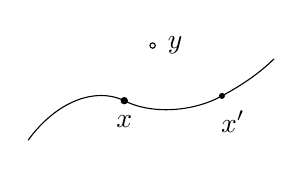
\begin{tikzpicture}[x=1cm,y=1cm,line cap=round]
\draw (0,0) .. controls (.35,.48) and (.84,.68) .. (1.22,.50)
.. controls (1.57,.32) and (2.10,.36) .. (2.46,.56)
.. controls (2.72,.70) and (2.95,.86) .. (3.12,1.03);
\fill (1.22,.50) circle (.047);
\fill (2.46,.56) circle (.038);
\draw (1.58,1.20) circle (.034);
\node[below] at (1.22,.43) {$x$};
\node[below] at (2.60,.49) {$x'$};
\node[right] at (1.65,1.20) {$y$};
\end{tikzpicture}}\endgroup
}
\end{GelfandAdjacentEvidence}
\begin{GelfandAdjacentEvidence}{GELFAND-P000988}{3}


$(x,y)\mapsto(x,x')$ is impossible, since $\{x\}^{\mathrm{cl}}$ is pres.\textsuperscript{?}
\Unclear{GELFAND-P000988}{impossible-tail}{pres.}
\end{GelfandAdjacentEvidence}
\begin{GelfandAdjacentEvidence}{GELFAND-P000988}{4}


On $\overline{\mathcal F}_I$ it can already act doubly transitively

\underline{Example}

doubly trans. on $F\Longleftrightarrow$ trans. on $(F\times F)\setminus\Delta$
\[
\forall x\in F,\quad G_x\text{ must act transitively on }F\setminus\{x\}
\]
\SourceFigure{GELFAND-P000988}{diagonal-sketch}{A quadrilateral with a rising diagonal and a small gap in its upper left corner.\par\smallskip
\begingroup\color{black}\GelfandFitDiagram{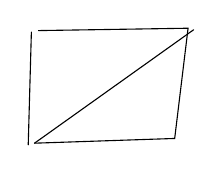
\begin{tikzpicture}[x=1cm,y=1cm,line cap=round]
\draw (0,0)--(.04,1.43);
\draw (.13,1.45)--(2.03,1.48)--(1.86,.08)--(.08,.02);
\draw (.08,.02)--(2.10,1.46);
\end{tikzpicture}}\endgroup
}
\end{GelfandAdjacentEvidence}
\begin{GelfandAdjacentEvidence}{GELFAND-P000988}{5}


The end will be as follows: for

$B,N,T,W,P$

an axiomatic generalization is given, for which the Bruhat decomp. makes sense.

\underline{Under certain conditions on the action:}

(i)
\[
\mathcal F_{\max}=\{\max\ \text{totally ordered chain}\quad
S_1<S_2<\cdots<S_i<\cdots
\]
[Crossed out at the end of the line: entry unresolved.]
\Unclear{GELFAND-P000988}{axiom1-cancel-end}{entry unresolved}
\end{GelfandAdjacentEvidence}
\begin{GelfandAdjacentEvidence}{GELFAND-P000988}{6}


$S_i\in$ [crossed out: entry unresolved] $\mathcal F\}$
\Unclear{GELFAND-P000988}{axiom1-cancel-family}{entry unresolved}
\end{GelfandAdjacentEvidence}
\begin{GelfandAdjacentEvidence}{GELFAND-P000988}{7}


[Below $\mathcal F_{\max}$:] (Flags)

\SourceFigure{GELFAND-P000988}{flags-max-symbol}{There is no distinct bar above $\mathcal F_{\max}$.}
\end{GelfandAdjacentEvidence}
\begin{GelfandAdjacentEvidence}{GELFAND-P000988}{8}


\underline{trans. with respect to $G$}

(ii)
\[
\forall S:\ \dim(S)=\text{length of a $\max$ flag},\quad<+\infty
\]
[Below $S$, $\mathcal F$ is added with an upward arrow.]\SourceFigure{GELFAND-P000988}{dimension-pointer}{The arrow points up from $\mathcal F$ to $S$.}
\end{GelfandAdjacentEvidence}
\begin{GelfandAdjacentEvidence}{GELFAND-P000988}{9}


[Crossed out below $\dim(S)$: entry unresolved.]
\Unclear{GELFAND-P000988}{axiom2-cancel-under-dim}{entry unresolved}
\end{GelfandAdjacentEvidence}
\begin{GelfandAdjacentEvidence}{GELFAND-P000988}{10}


[Below “length of a $\max$ flag”: unresolved entry crossed out, then:] ending in $S$.
\Unclear{GELFAND-P000988}{axiom2-cancel-before-ending}{unresolved entry}
\end{GelfandAdjacentEvidence}
\begin{GelfandAdjacentEvidence}{GELFAND-P000988}{11}


(iii)
\[
S,S'\subseteq T,\quad\dim S+\dim S'>\dim(T)
\Rightarrow S\cap S'\ne\bigcap_{\mathcal F\ni T'}T'
\]
(iv) $\forall S\in\mathcal F$, if $\{x\}^{\mathrm{cl}}\cap S=$ $(\varnothing)^{\mathrm{cl}}$\textsuperscript{?}, then
\[
G^S\cap G^{\{x\}^{\mathrm{cl}}}
\underset{\text{maps \underline{\underline{onto}}}}{\longrightarrow}
\overline{G^S}
\]
\Unclear{GELFAND-P000988}{axiom4-zero}{$(\varnothing)^{\mathrm{cl}}$}
\end{GelfandAdjacentEvidence}
\begin{GelfandAdjacentEvidence}{GELFAND-P000988}{12}

Then
\[
G=\coprod_WG^f wG^f\qquad\text{(disjoint union)}
\]
(double coset)

where
\[
G^f=\bigcap_I G^{f(i)},\qquad f:I\to\mathcal F
\]
[A leader from $G^f$ to the caption:] stabilizer of a $\max$ flag.
\[
W=N/T
\]
[“Here” is written above $f$.]
\[
\{f:I\to\mathcal F;\quad S_1<S_2<S_3<S_4<\cdots
\]
--- any $\max$ chain $\}$ \SourceFigure{GELFAND-P000988}{bottom-left-arrow}{A short stroke precedes “any”. No separate arrowhead is discernible.}
\end{GelfandAdjacentEvidence}



\Needspace{7\baselineskip}
\begin{GelfandAdjacentEvidence}{GELFAND-P000989}{1}
\SourcePage{GELFAND-P000989}{unlabelled}
\underline{Problems.} (I.M.G.)

Describe the 2-sided cosets
\[
\begin{aligned}
1)&\quad U(n)\backslash GL(n)/U(n)\\
2)&\quad \underset{\substack{\diagup\\\text{triang.}}}{B(n)}
             \backslash GL(n)/B(n)\\
3)&\quad U(n)\backslash GL(n)/B(n)
\end{aligned}
\]
\SourceFigure{GELFAND-P000989}{double-coset-leader}{An oblique leader connects “triang.” to the left $B(n)$ in item 2.}
\end{GelfandAdjacentEvidence}
\begin{GelfandAdjacentEvidence}{GELFAND-P000989}{2}


Every $\max$ flag is obtained as follows:
\[
f(i)=\operatorname{cl}(\{e_j\}_{j\leq i}),\quad
\text{where }\{e_j\}\text{ are points in }X.
\]
\[
C_i=\operatorname{cl}(\{e_i\})
\]
\[
N=\{g\mid g\text{ permutes }\{C_i\}\}
\]
and we have:

\SourceFigure{GELFAND-P000989}{middle-group-sequence}{The initial symbol is overwritten. Tentatively $1$ over $0$.\par\smallskip
\begingroup\color{black}\GelfandFitDiagram{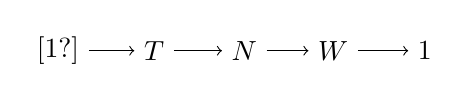
\begin{tikzpicture}[baseline=(a.base), x=.91cm]
\node (a) at (0,0) {$[1?]$};
\node (t) at (1.34,0) {$T$};
\node (n) at (2.60,0) {$N$};
\node (w) at (3.84,0) {$W$};
\node (one) at (5.12,0) {$1$};
\draw[->] (a)--(t);
\draw[->] (t)--(n);
\draw[->] (n)--(w);
\draw[->] (w)--(one);
\end{tikzpicture}}\endgroup
}
\end{GelfandAdjacentEvidence}
\begin{GelfandAdjacentEvidence}{GELFAND-P000989}{3}


$T$ consists of those that leave each $C_i$ in place;

$W=N/T$ by def.

The speaker knows of no examples other than the classical ones where all the axioms hold.

But: there are examples where the decomp. [crossed out: not (?)] exists, although the axioms do not hold.
\Unclear{GELFAND-P000989}{lower-cancelled-word}{not (?)}
\end{GelfandAdjacentEvidence}
\begin{GelfandAdjacentEvidence}{GELFAND-P000989}{4}


\underline{Zelevinsky.}

On the paper by \underline{S. Abeasis, A. Del Fra, H. Kraft.}

\underline{The geometry of repres. of $A_m$}, Math. Ann., 256, N.3,
401--418, (1981).

\SourceFigure{GELFAND-P000989}{lower-bibliography-pages}{The opening page reads $401$.}
\end{GelfandAdjacentEvidence}
\begin{GelfandAdjacentEvidence}{GELFAND-P000989}{5}


$A_m$ --- a quiver

\SourceFigure{GELFAND-P000989}{lower-quiver}{The last arrow has a right-pointing head and additional strokes at the left end. Its label is $A_m$.\par\smallskip
\begingroup\color{black}\GelfandFitDiagram{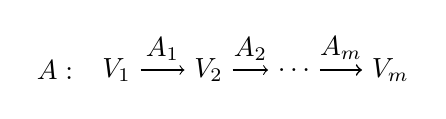
\begin{tikzpicture}[baseline=(a.base), x=.92cm]
\node (a) at (0,0) {$A:$};
\node (first) at (.85,0) {$V_1$};
\node (second) at (2.12,0) {$V_2$};
\node (dots) at (3.30,0) {$\ldots$};
\node (last) at (4.63,0) {$V_m$};
\draw[->] (first)--node[above] {$A_1$} (second);
\draw[->] (second)--node[above] {$A_2$} (dots);
\draw[->,semithick] (dots)--node[above] {$A_m$} (last);
\end{tikzpicture}}\endgroup
}
\end{GelfandAdjacentEvidence}
\begin{GelfandAdjacentEvidence}{GELFAND-P000989}{6}


--- this is a rep. of a quiver of series $A_m$.

Here the group acts
\[
GL(V_1)\times\cdots\times GL(V_m).
\]
\SourceFigure{GELFAND-P000989}{bottom-group-index}{The first subscript reads $1$.}
\end{GelfandAdjacentEvidence}
\begin{GelfandAdjacentEvidence}{GELFAND-P000989}{7}


Orbits are reps. up to equiv.

There are finitely many orbits. They admit\textsuperscript{?} an explicit descr.
\Unclear{GELFAND-P000989}{bottom-description-abbrev}{admit}
\end{GelfandAdjacentEvidence}
\begin{GelfandAdjacentEvidence}{GELFAND-P000989}{8}


Their closures are good varieties (normal, Cohen---Macaulay\textsuperscript{?}, etc.).
\Unclear{GELFAND-P000989}{bottom-cohen-macaulay}{Macaulay}
\end{GelfandAdjacentEvidence}



\Needspace{7\baselineskip}
\begin{GelfandAdjacentEvidence}{GELFAND-P000990}{1}
\SourcePage{GELFAND-P000990}{16}
[Crossed out: Their (?)] They are analogous to Schubert cells, and the polynomials describe reps. of $p$-adic groups, as the geom. of Schubert cells is connected with reps. of classical groups.
\Unclear{GELFAND-P000990}{top-cancelled-word}{Their (?)}
\end{GelfandAdjacentEvidence}
\begin{GelfandAdjacentEvidence}{GELFAND-P000990}{2}


For

\SourceFigure{GELFAND-P000990}{first-linear-arrow}{The arrow from $V_1$ to $V_2$ is labelled $A_1$.\par\smallskip
\begingroup\color{black}\GelfandFitDiagram{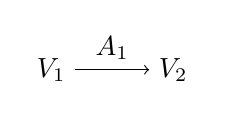
\begin{tikzpicture}[baseline=(first.base)]
\node (first) at (0,0) {$V_1$};
\node (second) at (1.55,0) {$V_2$};
\draw[->] (first)--node[above] {$A_1$} (second);
\end{tikzpicture}}\endgroup
}
\end{GelfandAdjacentEvidence}
\begin{GelfandAdjacentEvidence}{GELFAND-P000990}{3}

determinantal varieties arise.

Description of orbits:

\SourceFigure{GELFAND-P000990}{upper-composition-arrow}{A separate, overtraced mark lies below $V_i$. Its reading is unresolved.\par\smallskip
\begingroup\color{black}\GelfandFitDiagram{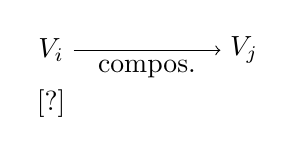
\begin{tikzpicture}[baseline=(first.base)]
\node (first) at (0,0) {$V_i$};
\node (second) at (2.45,0) {$V_j$};
\draw[->] (first)--node[below] {compos.} (second);
\node[below=3pt] at (first.south) {$[?]$};
\end{tikzpicture}}\endgroup
}
\end{GelfandAdjacentEvidence}
\begin{GelfandAdjacentEvidence}{GELFAND-P000990}{4}


Specify the \underline{ranks of all possible compositions} $r_{ij}$.

A system of inequalities must hold.

There is another descr. via multiplicities of occurrences.

\underline{\underline{19/X-81.}}\qquad\underline{Gelfand Sem.}

\underline{Kirillov.}

How is the Lie algebra with generators $x,y$ and rels. structured?
\[
(\operatorname{ad}x)^{a+1}y=0,\qquad
(\operatorname{ad}y)^{b+1}x=0,\qquad a,b\in\mathbb{N}.
\]
\SourceFigure{GELFAND-P000990}{dimension-table}{The $a$ axis points right and $b$ down. The entries $(a,b)=(3,2),(2,3)$ are question marks. Blank entries remain blank.\par\smallskip
\begingroup\color{black}\GelfandFitDiagram{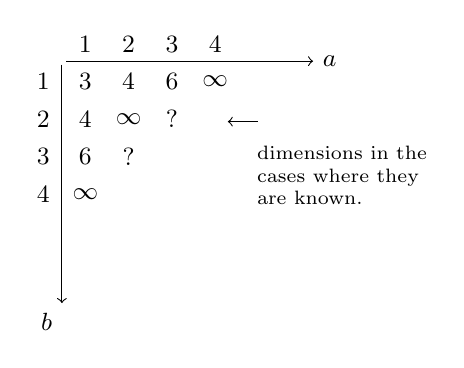
\begin{tikzpicture}[x=.55cm,y=.48cm,font=\small]
\draw[->] (.1,0)--(5.8,0) node[right] {$a$};
\draw[->] (0,-.09)--(0,-6.4) node[below left] {$b$};
\foreach \i in {1,2,3,4} {
 \node at (\i-.46,.43) {$\i$};
 \node at (-.43,-\i+.47) {$\i$};
}
\node at (.54,-.53) {$3$};
\node at (1.54,-.53) {$4$};
\node at (2.54,-.53) {$6$};
\node at (3.54,-.53) {$\infty$};
\node at (.54,-1.53) {$4$};
\node at (1.54,-1.53) {$\infty$};
\node at (2.54,-1.53) {$?$};
\node at (.54,-2.53) {$6$};
\node at (1.54,-2.53) {$?$};
\node at (.54,-3.53) {$\infty$};
\draw[<-] (3.83,-1.60)--(4.53,-1.60);
\node[anchor=north west,align=left,font=\scriptsize] at (4.28,-2.00) {dimensions in the\\cases where they\\are known.};
\end{tikzpicture}}\endgroup
}
\end{GelfandAdjacentEvidence}
\begin{GelfandAdjacentEvidence}{GELFAND-P000990}{5}


\underline{Without relations}, the number of commutators of bidegree $k,\ell$ is:
\[
d(k,\ell)=\frac{1}{k+\ell}\sum_{d\mid(k,\ell)}
\mu(d)\,\frac{\left(\frac{k}{d}+\frac{\ell}{d}\right)!}
{\frac{k}{d}!\,\frac{\ell}{d}!}.
\]
$k=n$, $\ell=n+1$ $\Rightarrow$ the $n$th Catalan number

($=$ the number of ways of placing parentheses in the nonassoc. product $x\cdot x\cdot\ldots\cdot x$.)

[At left above the next line: $(\sim)$.]

Another question: the envelop. algebra.

\underline{Rels.}
\begin{align*}
0&=x^{a+1}y-\binom{a+1}{1}x^ayx+\binom{a+1}{2}x^{a-1}yx^2+\ldots\,,\\
0&=y^{b+1}x-\binom{b+1}{1}y^bxy+\binom{b+1}{2}y^{b-1}xy^2-\ldots\,.
\end{align*}
\SourceFigure{GELFAND-P000990}{lower-relation-signs}{Before the ellipsis the first line has $+$ and the second $-$.}
\end{GelfandAdjacentEvidence}
\begin{GelfandAdjacentEvidence}{GELFAND-P000990}{6}


$V$ --- a vector space, \qquad $S(\bar V)=e^{\bar V}$ --- the symm. algebra

[Below “$V$ --- a vector space”: “(graded)”.]

$p(t)=\sum t^k\dim V_k$ --- the Hilbert polynomial.
\Unclear{GELFAND-P000990}{bottom-hilbert-letter}{$p(t)$}
\end{GelfandAdjacentEvidence}



\Needspace{7\baselineskip}
\begin{GelfandAdjacentEvidence}{GELFAND-P000991}{1}
\SourcePage{GELFAND-P000991}{unlabelled}
$k$ --- a weight $\Rightarrow$ a weight arises on $S(V)$
$\Rightarrow$ grading on $S(V)$
$\Rightarrow$ the Hilbert polynomial is calculated $P(t)$ for $S(V)$
(or a formal series).

Relation:

[Crossed out: formula unresolved.]
\Unclear{GELFAND-P000991}{series-cancelled-01}{formula unresolved}
\end{GelfandAdjacentEvidence}
\begin{GelfandAdjacentEvidence}{GELFAND-P000991}{2}

\[
\ln P(t)=\sum\frac{C_k}{k}t^k;
\]
[Crossed out: short entry unresolved.]
\Unclear{GELFAND-P000991}{series-cancelled-02}{short entry unresolved}
\end{GelfandAdjacentEvidence}
\begin{GelfandAdjacentEvidence}{GELFAND-P000991}{3}

\[
p(t)=\sum\frac{c_k}{k}t^k,\qquad C_k=\sum_{d\mid k}c_d.
\]
\SourceFigure{GELFAND-P000991}{series-coefficient}{In the expression for $p(t)$ the denominator is $k$ and the numerator is $c_k$.}
\end{GelfandAdjacentEvidence}
\begin{GelfandAdjacentEvidence}{GELFAND-P000991}{4}

\[
\underline{x^{k_1}y^{\ell_1}x^{k_2}y^{\ell_2}\ldots x^{k_n}y^{\ell_n}}
\]
\[
\begin{aligned}
k_1+k_2+\ldots+k_n&=k,\\
\ell_1+\ell_2+\ldots+\ell_n&=\ell.
\end{aligned}
\]
Lexicographic ordering.

\underline{$y$ is higher than $x$}. \qquad $x<y$.

\underline{I.M.G.} \quad \underline{combin. problem}

$m_1\le m_2\le m_3\le m_4$ --- \underline{fixed}

\SourceFigure{GELFAND-P000991}{table-interlacing}{Four rows of circles with $4,3,2,1$ entries. The pointer from the note at left marks the first circle of the second row.\par\smallskip
\begingroup\color{black}\GelfandFitDiagram{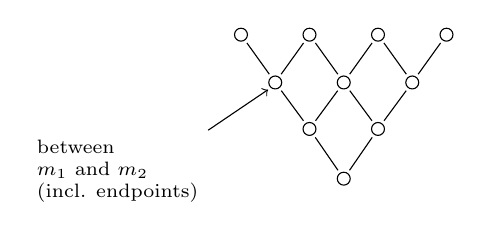
\begin{tikzpicture}[x=.87cm,y=.82cm,
  dot/.style={circle,draw,inner sep=1.65pt,outer sep=1.35pt}]
\node[dot] (a1) at (0,0) {};
\node[dot] (a2) at (1,0) {};
\node[dot] (a3) at (2,0) {};
\node[dot] (a4) at (3,0) {};
\node[dot] (b1) at (.50,-.74) {};
\node[dot] (b2) at (1.50,-.74) {};
\node[dot] (b3) at (2.50,-.74) {};
\node[dot] (c1) at (1,-1.46) {};
\node[dot] (c2) at (2,-1.46) {};
\node[dot] (d1) at (1.50,-2.23) {};
\draw (a1)--(b1)--(a2)--(b2)--(a3)--(b3)--(a4);
\draw (b1)--(c1)--(b2)--(c2)--(b3);
\draw (c1)--(d1)--(c2);
\node[align=left,anchor=north east,font=\scriptsize] (note) at (-.48,-1.48)
  {between\\$m_1$ and $m_2$\\(incl. endpoints)};
\draw[->] (note.north east)--(b1.south west);
\end{tikzpicture}}\endgroup
}
\end{GelfandAdjacentEvidence}


\underline{how many tables?}

($=$ how many reps. of $SL(4)$ with a given highest weight?)

see the appendix to the Gelfand–Minlos–Shapiro book.


\Needspace{7\baselineskip}
\begin{GelfandAdjacentEvidence}{GELFAND-P000992}{1}
\SourcePage{GELFAND-P000992}{unlabelled}
\underline{\underline{16.11.81.}} \qquad \underline{Gelfand Sem.}

\underline{\underline{A.S. Schwarz.}} \qquad \underline{Geometry of supergravity.}

$\mathbb R^{p,q}$ --- superspace\qquad
$(x^1,\ldots,x^p,\theta^1,\ldots,\theta^q)$.

$\Lambda$ --- Grassmann alg.
[Above the abbreviation: г or 4\textsuperscript{?}.]
\Unclear{GELFAND-P000992}{algebra-insertion}{г or 4}
\end{GelfandAdjacentEvidence}
\begin{GelfandAdjacentEvidence}{GELFAND-P000992}{2}

[Crossed out: entry unresolved.]
\Unclear{GELFAND-P000992}{algebra-cancelled-01}{entry unresolved}
\end{GelfandAdjacentEvidence}
\begin{GelfandAdjacentEvidence}{GELFAND-P000992}{3}

[Crossed out: with grading\textsuperscript{?}.]
\Unclear{GELFAND-P000992}{algebra-cancelled-02}{with grading}
\end{GelfandAdjacentEvidence}
\begin{GelfandAdjacentEvidence}{GELFAND-P000992}{4}

(over $\mathbb R$).

$\mathbb R^{p,q}_{\Lambda}$ --- the space of rows
$(x^1,\ldots,x^p,\theta^1,\ldots,\theta^q)$,
where $x^j$ are even elems. of $\Lambda$, $\theta^j$ are odd elems. of $\Lambda$.

We need to consider this as a functor of $\Lambda$ (it is inconvenient\textsuperscript{?} to fix $\Lambda$).
\Unclear{GELFAND-P000992}{functor-parenthesis}{inconvenient}
\end{GelfandAdjacentEvidence}
\begin{GelfandAdjacentEvidence}{GELFAND-P000992}{5}


This gives $\mathbb R^{p,q}$.

$\mathbb C^{p,q}$ is def. analogously and an involution is def. in it.

\medskip
Consider $\mathbb C^{4,2}$ \qquad $(x^m,\theta^\alpha)=z^A$.
\[
\dim_{\mathbb C}\mathbb C^{4,2}=(4,2),\qquad
\dim_{\mathbb R}(\mathbb C^{4,2})=(8,4).
\]
In it consider a real subvariety
\[
\begin{array}{cl}
\Omega & \subset\mathbb C^{4,2}\\[-1pt]
(4,4)&\leftarrow\underline{\mathbb R}\text{-dim}
\end{array}
\]
\SourceFigure{GELFAND-P000992}{omega-dimension}{Below $\Omega$ the manuscript has $(4,4)$, with an arrow pointing to it from $\underline{\mathbb R}$-dim.}
\end{GelfandAdjacentEvidence}


$\Omega$ is cut out by the eqs.
\[
f^k(z,\bar z)=0,
\]
$f^k$ are even and real, \quad $k=1,2,3,4$.

Consider analytic transformations in $\mathbb C^{4,2}$:
\[
\begin{cases}
\widetilde{x}^{a}=\lambda^{a}(x,\theta),\\
\widetilde{\theta}^{\alpha}=\lambda^{\alpha}(x,\theta)
\end{cases}
\qquad
\text{(indep. of $\bar x,\bar\theta$)}.
\]


\Needspace{7\baselineskip}
\begin{GelfandAdjacentEvidence}{GELFAND-P000993}{1}
\SourcePage{GELFAND-P000993}{40}
They form a supergroup $L$.

(The group depends on $\Lambda$ and all together --- a functor from Grassmann algs. to ordinary groups --- supergroups.)

Consider those that preserve the \underline{supervolume}.
\[
\widetilde z^{A}=\lambda^{A}(z).
\]
Preservation of volume:
\[
\operatorname{Ber}\frac{\partial\widetilde z^{A}}{\partial z^{B}}=1.
\]
We shall consider the functional
\[
S(\Omega)=\int A\bigl(\text{first, second derivs. of }f^k\bigr)
\prod_k\delta\bigl(f^k(z,\bar z)\bigr)\,dz\,d\bar z.
\]
[In the argument of $A$, before $f^k$, crossed out: $f^k$\textsuperscript{?}.]
\Unclear{GELFAND-P000993}{functional-cancelled}{$f^k$}
\end{GelfandAdjacentEvidence}
\begin{GelfandAdjacentEvidence}{GELFAND-P000993}{2}


[A leader to $\delta$ is labelled “$\delta$-fn.”.]\SourceFigure{GELFAND-P000993}{delta-label}{The gloss “$\delta$-fn.” is below $\delta$.}
\end{GelfandAdjacentEvidence}
\begin{GelfandAdjacentEvidence}{GELFAND-P000993}{3}


Impose a condition on $A$ so that $S(\Omega)$ depends only on $\Omega$, rather than on its eqs.

In classical field theory, in place of the field $\varphi$ one can consider the graph of the fn. --- a surface.

\SourceFigure{GELFAND-P000993}{field-graph}{A graph with its minimum above the horizontal $x$-axis and a vertical $\varphi$-axis.\par\smallskip
\begingroup\color{black}\GelfandFitDiagram{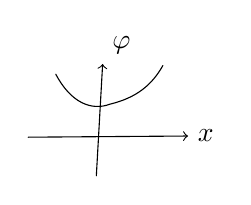
\begin{tikzpicture}[x=1cm,y=1cm,line cap=round]
\draw[->] (-.90,0)--(1.13,.015) node[right] {$x$};
\draw[->] (-.035,-.49)--(.045,.93) node[above right] {$\varphi$};
\draw (-.55,.80) .. controls (-.36,.44) and (-.10,.33) .. (.14,.42)
 .. controls (.47,.50) and (.67,.66) .. (.81,.91);
\end{tikzpicture}}\endgroup
}
\end{GelfandAdjacentEvidence}
\begin{GelfandAdjacentEvidence}{GELFAND-P000993}{4}


Consider $\Omega$ as the graph of the field
\[
\mathbb R^{4,4}\longrightarrow\mathbb R^{4,0},\qquad
H^m(\xi,\theta,\bar\theta).
\]
\Unclear{GELFAND-P000993}{superfield-argument}{The first argument is heavily retraced. The tentative reading is $\xi$.}
\end{GelfandAdjacentEvidence}
\begin{GelfandAdjacentEvidence}{GELFAND-P000993}{5}


The surf. $\Omega$ and the superfield are in one-to-one corresp.

\underline{Supergravity action:} the \underline{unique} (up to a factor) functional \underline{of this kind invariant with respect to the group $L$}.

Then by varying $S(\Omega)$ we obtain\textsuperscript{?}.
\Unclear{GELFAND-P000993}{variation-last-word}{obtain}
\end{GelfandAdjacentEvidence}
\begin{GelfandAdjacentEvidence}{GELFAND-P000993}{6}


Namely:
\[
A=|\det\Gamma|^{-1/2},\qquad
\Gamma\text{ is the Levi form of the surface }\Omega.
\]
\SourceFigure{GELFAND-P000993}{levi-power}{A minus sign precedes the fraction $1/2$.}
\end{GelfandAdjacentEvidence}
\begin{GelfandAdjacentEvidence}{GELFAND-P000993}{7}


[“(super.)” is inserted beneath “form”.]

The Levi form is the first \underline{struct. form} of the $CR$-structure.

The form
\[
\left.
\frac{\partial^2 f^k}{\partial z^A\partial\bar z^B}\,
dz^A\,d\bar z^B
\ \right|_{\substack{\text{on the compl. tangent plane}\\
 \frac{\partial f^k}{\partial z^A}dz^A=0}}
\]
(vector-valued)

[Crossed out: $\partial f$.]\SourceFigure{GELFAND-P000993}{levi-cancellation}{Above “called the Levi form”, $\partial f$ is crossed out.}
\end{GelfandAdjacentEvidence}
\begin{GelfandAdjacentEvidence}{GELFAND-P000993}{8}


\underline{is called the Levi form $\Gamma$}.

\SourceFigure{GELFAND-P000993}{levi-pointer}{A downward arrow from the words about the tangent plane leads to the dimensional note.}
\end{GelfandAdjacentEvidence}


it has dimension $(0,2)$.
\[
\frac{\partial f^k}{\partial x^a}\,dx^a+
\frac{\partial f^k}{\partial\theta^\alpha}\,d\theta^\alpha=0
\]
\[
\Rightarrow dx^a\text{ is expressed in terms of }d\theta^\alpha
\Rightarrow \text{dim. }(0,2).
\]


\Needspace{7\baselineskip}
\begin{GelfandAdjacentEvidence}{GELFAND-P000994}{1}
\SourcePage{GELFAND-P000994}{unlabelled}
The basis in the compl. tangent plane is chosen in different ways.

Det. (?) depends on this.
\Unclear{GELFAND-P000994}{det-overwritten}{The initial strokes of “Det.” are overwritten.}
\end{GelfandAdjacentEvidence}
\begin{GelfandAdjacentEvidence}{GELFAND-P000994}{2}

\[
\Gamma^k_{\alpha\dot\beta}
\qquad
\begin{aligned}
k&\text{ --- 4 possibilities},\\
\alpha,\dot\beta&\text{ --- 4 possibilities}\quad(2\times2=4).
\end{aligned}
\]
\SourceFigure{GELFAND-P000994}{levi-indices}{In the subscript of $\Gamma$ the dot is above $\beta$.}
\end{GelfandAdjacentEvidence}
\begin{GelfandAdjacentEvidence}{GELFAND-P000994}{3}

\underline{\underline{$\det$}} --- $\det$ \underline{such a $4\times4$ matrix}.

It and $\det$ depend on the choice of basis.

One must [crossed out: illegible] choose the basis correctly in the compl. tangent plane.
\Unclear{GELFAND-P000994}{basis-cancelled}{The entry after “One must” is crossed out. Its reading is unresolved.}
\end{GelfandAdjacentEvidence}
\begin{GelfandAdjacentEvidence}{GELFAND-P000994}{4}


For functions: natural choice of basis
\[
\Gamma^k_{\alpha\dot\beta}\,d\theta^\alpha\,d\overline{\theta^\beta}.
\]
\Unclear{GELFAND-P000994}{levi-differential-index}{The reach of the overbar and the dot at the superscript of the second differential are unclear: $d\overline{\theta^\beta}$ or $d\bar\theta^{\dot\beta}$.}
\end{GelfandAdjacentEvidence}
\begin{GelfandAdjacentEvidence}{GELFAND-P000994}{5}


and then one must write
\[
A=\left(\det\frac{\partial f^k}{\partial z^a}\right)^{4/3}
|\det\Gamma|^{-1/3}.
\]
\Unclear{GELFAND-P000994}{density-denominator}{The denominator tentatively reads $z^a$, possibly $x^a$. The letter is overwritten.}
\end{GelfandAdjacentEvidence}
\begin{GelfandAdjacentEvidence}{GELFAND-P000994}{6}


see \underline{Yadernaya Fizika}, 1981, $N=10$.

prelim. large (?) work. \underline{Nuclear Physics}, 1981.

[A right bracket groups the two references, with the label:] \underline{A.S. Schwarz}.

[At right:] there is also something in \underline{Communic. Math. Phys.}
\SourceFigure{GELFAND-P000994}{bibliography-brace}{The name and a separate note on a journal stand to the right of the bracket.}
\end{GelfandAdjacentEvidence}
\begin{GelfandAdjacentEvidence}{GELFAND-P000994}{7}

\Unclear{GELFAND-P000994}{bibliography-abbreviations}{Before “Nuclear Physics”, tentatively “prelim. large work”.}
\end{GelfandAdjacentEvidence}
\begin{GelfandAdjacentEvidence}{GELFAND-P000994}{8}


$G$-struct. on a compl. manifold (abbrev. uncertain) $\Rightarrow CR$ structure on the surface.
\Unclear{GELFAND-P000994}{manifold-abbreviation}{After “on a compl.” the manuscript uses a hyphenated abbreviation, tentatively “мн-зии”.}
\end{GelfandAdjacentEvidence}


($\sim$ compl. str. $GL(n,\mathbb C)$)

Here $SL(4,2\mid\mathbb C)$ is the structure.

$L$ is the autom. group of this struct.

An $SCR$ structure arises on the surf., differing from $CR$ by the $\det$ condition.

In $\mathbb C^{4,2}$ the coordinates and the field values are mixed up, and they cannot be considered separately.

\begin{center}$-\ \cdot\ -$\end{center}


\Needspace{7\baselineskip}
\begin{GelfandAdjacentEvidence}{GELFAND-P000995}{1}
\SourcePage{GELFAND-P000995}{unlabelled}
\underline{23.11.81}\qquad\underline{\underline{Gelfand Sem.}}

\underline{Zelevinsky}.

$\mathfrak g$ --- compl. semis. Lie alg.
\[
\mathfrak g\supset
\underset{\text{Borel}}{\mathfrak b}\supset
\underset{\text{Cartan}}{\mathfrak h}.
\]
\underline{Example.}\quad $\mathfrak{sl}_n$\qquad [below $\mathfrak b$: “upper triang.”, below $\mathfrak h$: “diag.”].
\[
\underbrace{
 \overbrace{e_1,\ldots,e_n}^{\mathfrak n_+},
 \overbrace{h_1,\ldots,h_n}^{\mathfrak h}
}_{\mathfrak b_+},
\quad f_1,\ldots,f_n.
\]
\SourceFigure{GELFAND-P000995}{generator-brackets}{The two upper brackets are marked $\mathfrak n_+$ and $\mathfrak h$ and the common lower bracket is marked $\mathfrak b_+$.}
\end{GelfandAdjacentEvidence}
\begin{GelfandAdjacentEvidence}{GELFAND-P000995}{2}


\underline{Rep.:} $e_j\mapsto E_j$ etc.

Highest weight! vector $x$: $E_jx=0$, $j=1,\ldots,n$.
\SourceFigure{GELFAND-P000995}{highest-weight-exclamation}{The mark after “weight” reads as an exclamation mark.}
\end{GelfandAdjacentEvidence}
\begin{GelfandAdjacentEvidence}{GELFAND-P000995}{3}


$\Rightarrow H_jx$ --- also a highest weight.

Always $\exists$ in a finite-dimensional rep.

\underline{Verma module}

$\chi\in\mathfrak h^*$.

[Crossed out: “Highest” (abbrev., tentative)] Vector of highest weight $\chi$:
\[
\begin{cases}
ev=0,&\forall e\in\mathfrak n_+,\\
hv=\chi(h)v,&\forall h\in\mathfrak h.
\end{cases}
\]
\Unclear{GELFAND-P000995}{highest-weight-cancelled}{The crossed-out entry tentatively reads “Highest” in abbreviation.}
\end{GelfandAdjacentEvidence}
\begin{GelfandAdjacentEvidence}{GELFAND-P000995}{4}


\underline{Verma module:} the largest module $M(\chi)$ gen. by highest weight $\chi$.

(Universal module with these props.)

$M(\chi)$ is not irreduc. (generally speaking).

$L(\chi)$ --- the unique irreduc. quotient module of $M(\chi)$.

\underline{Thm.} $\exists$ a finite compos. series
\[
M(\chi)=M_1\supset M_2\supset\ldots\supset M_n=0,
\qquad M_i/M_{i+1}=L(\chi_i).
\]
$\Rightarrow$ every subquotient has this form.

\underline{Question:} given $\psi$, what is the multiplicity of occurrence of $M(\psi)$ in the compos. series of a Verma mod.
\SourceFigure{GELFAND-P000995}{multiplicity-module-letter}{The question has $M(\psi)$.}
\end{GelfandAdjacentEvidence}
\begin{GelfandAdjacentEvidence}{GELFAND-P000995}{5}


(This is equiv. to describing the Verma mod. [inserted above: “itself”].)
[Below the parentheses: “--- can be calculated”.]
\SourceFigure{GELFAND-P000995}{itself-insertion}{The word “itself” is above the line with an insertion mark.}
\end{GelfandAdjacentEvidence}
\begin{GelfandAdjacentEvidence}{GELFAND-P000995}{6}


Denote the multiplicities
\[
m(\chi,\psi)=[M(\chi):L(\psi)].
\]

Multiplicities $=$ value of a certain polynomial at pt. 1.
\Unclear{GELFAND-P000995}{polynomial-abbreviation}{The word “certain” before “polynomial” is abbreviated.}
\end{GelfandAdjacentEvidence}
\begin{GelfandAdjacentEvidence}{GELFAND-P000995}{7}


\underline{Condition:}
\[
\chi+\rho\in W(\psi+\rho),\quad
\text{i.e.}\quad \chi+\rho=w(\psi+\rho).
\]
[Label at $W$: “Weyl gr.”]

$\rho$ is def. by the formula $\rho(h_i)=1$.

Only then can the multiplicity $m(\chi,\psi)$ be $\ne0$.

$\chi$ \underline{integral dominant} if $\lambda(h_i)\in\{0,1,2,\ldots\}$ for all $h_i$.
\SourceFigure{GELFAND-P000995}{dominance-variable}{After “if” the condition uses $\lambda(h_i)$, while the line begins with $\chi$.}
\end{GelfandAdjacentEvidence}



\Needspace{7\baselineskip}
\SourcePage{GELFAND-P000996}{46}
\underline{Our case:}

$\chi_0$ --- integral dominant, and
\begin{gather*}
\chi+\rho=w_1(\chi_0+\rho)\\
\psi+\rho=w_2(\chi_0+\rho)
\end{gather*}
Then
\[
m(\chi,\psi)=m(w_1,w_2)
\]
(does not depend on the choice of dominant weight $\chi_0$).


\begin{GelfandAdjacentEvidence}{GELFAND-P000996}{1}
\underline{Kazhdan--Lusztig} --- hypothet. expression.

Now proved: Beilinson, Bernstein. Brylinski, Kashiwara.

They wrote down:
\[
P_{w_1,w_2}(q)
\]
--- a polynomial (with nonneg. coefficients).

\underline{Conjecture}
\[
m(w_1,w_2)=P_{w_1,w_2}(1).
\]
\[
P_{w_1,w_2}(q)=\sum a_iq^i.
\]
Meaning of $a_i$ --- ?

Explanation: $\exists$ a Jantzen filtration
\[
M(\chi)\supset M_1\supset M_2\supset\cdots
\]
$a_i={}$ multiplicity of $L(\psi)$ in $M_i/M_{i+1}$.

\underline{Beilinson.}

\underline{Jantzen filtration.}

Dual module \({}^*M(\chi)\).

General definition: through category $O$.

$O$ is the cat. of finitely gen. mod., [added above the line: $\mathfrak h$-]diagonaliz., [crossed out: illegible], where [crossed out: illegible] [replacement above the line: $\mathfrak n_-$ (?) acts locally nilpotently].
\Unclear{GELFAND-P000996}{category-cancelled-01}{Dense strokes cross out the entry after “diagonaliz.”.}
\end{GelfandAdjacentEvidence}
\begin{GelfandAdjacentEvidence}{GELFAND-P000996}{2}

\Unclear{GELFAND-P000996}{category-cancelled-02}{The entry after “where” is crossed out. Its exact reading is unresolved.}
\end{GelfandAdjacentEvidence}
\begin{GelfandAdjacentEvidence}{GELFAND-P000996}{3}

\Unclear{GELFAND-P000996}{nilpotent-sign}{The sign after $\mathfrak n$ is overwritten. The reading “$-$” is tentative.}
\end{GelfandAdjacentEvidence}
\begin{GelfandAdjacentEvidence}{GELFAND-P000996}{4}


It has a natural involution $*:O\longrightarrow O$.

(The dual rep. is the \underline{dual space}. It is infinitely gen., but contains a \underline{subrep.} consisting of functions that transform finite-dimensionally under $\mathfrak h$.)
\SourceFigure{GELFAND-P000996}{dual-last-word}{The end of the line reads “transform finite-dimensionally”, abbreviated in the manuscript.}
\end{GelfandAdjacentEvidence}
\begin{GelfandAdjacentEvidence}{GELFAND-P000996}{5}


[Added with an arrow to the preceding line:] Here only $\mathfrak n_+$, and not $\mathfrak n_-$, but this makes no difference.
\SourceFigure{GELFAND-P000996}{margin-plus-minus}{The addition says $\mathfrak n_+$ followed by “and not $\mathfrak n_-$”.}
\end{GelfandAdjacentEvidence}
\begin{GelfandAdjacentEvidence}{GELFAND-P000996}{6}


\underline{S. Gelfand.}

On each $M(\chi)$ introduce a bilinear form with numerical values.
\[
M(\chi)\ni f_{i_1}\ldots f_{i_k}v,\qquad
v\text{ --- highest-weight vector}.
\]
\SourceFigure{GELFAND-P000996}{form-module-parentheses}{The weight in the notation before $\ni$ is in parentheses.}
\end{GelfandAdjacentEvidence}
\begin{GelfandAdjacentEvidence}{GELFAND-P000996}{7}

\[
(f_{i_1}\ldots f_{i_k}v,\ f_{j_1}\ldots f_{j_l}v)
=
\begin{cases}
0\quad\text{when }\{i\}\ne\{j\}
 & \text{--- (unordered sets)},\\
\bigl(e_{i_1\ldots i_k}f_{j_1\ldots j_l}v\bigr)/v
 & \text{(vector in numerator is a multiple of $v$)}.
\end{cases}
\]
\SourceFigure{GELFAND-P000996}{form-multiindices}{In the numerator each of the single letters $e$ and $f$ carries a sequence of indices.}
\end{GelfandAdjacentEvidence}



\Needspace{7\baselineskip}
\begin{GelfandAdjacentEvidence}{GELFAND-P000997}{1}
\SourcePage{GELFAND-P000997}{unlabelled}
We obtain a form invar. with respect to the Lie alg.

[Crossed out: illegible] We will identify all $M(\chi)$ (for different $\chi$) as follows
\[
f_{i_1}\ldots f_{i_l}v_\chi
\longrightarrow f_{i_1}\ldots f_{i_l}v_{\chi'}.
\]
\Unclear{GELFAND-P000997}{top-cancelled}{A short entry before “We will” is crossed out.}
\end{GelfandAdjacentEvidence}
\begin{GelfandAdjacentEvidence}{GELFAND-P000997}{2}


Consider $M(\chi)$ with [crossed out: illegible] fixed $\chi$ and then consider $M(\chi+t\rho)$.
\Unclear{GELFAND-P000997}{fixed-cancel}{A short entry is crossed out between “with” and “fixed”.}
\end{GelfandAdjacentEvidence}
\begin{GelfandAdjacentEvidence}{GELFAND-P000997}{3}


We obtain many bilinear forms on one space:
\[
(\ ,\ )_t.
\]
Regard them all as forms on $M(\chi)$.

For small $t\ne0$ the form is nondegenerate.

\underline{Def.}
\[
M_i=\{x\in M_\chi\mid (x,y)_t=O(t^i)\}.
\]
[Above the condition, with an insertion mark:] $\forall y\in M(\chi):$
\SourceFigure{GELFAND-P000997}{filtration-quantifier}{The condition has the insertion $\forall y\in M(\chi)$ followed by a colon.}
\end{GelfandAdjacentEvidence}
\begin{GelfandAdjacentEvidence}{GELFAND-P000997}{4}


This is the Jantzen filtr.

It is a filtr. by $\mathfrak g$-submodules.

What if we change $\rho$? Apparently the mult. will remain the same.

Polynomial
\[
P_{w_1,w_2}(q)=\sum q^i\bigl([L_\psi:M_i/M_{i+1}]\bigr),
\]
\SourceFigure{GELFAND-P000997}{multiplicity-order}{The manuscript puts $L_\psi$ before the colon and $M_i/M_{i+1}$ after it.}
\end{GelfandAdjacentEvidence}
\begin{GelfandAdjacentEvidence}{GELFAND-P000997}{5}


where
\begin{gather*}
\psi=w_2(\chi_0+\rho)-\rho,\\
M_i\subset M_\chi,\qquad\chi=w_1(\chi_0+\rho)-\rho.
\end{gather*}
$P_{w_1,w_2}$ --- are determined recurr..
\[
a_i=\dim H^i\bigl(\text{of one Schubert cell near another, according to MacPherson}\bigr).
\]
(local cohomol. of a normal section)
\SourceFigure{GELFAND-P000997}{normal-section-sketch}{A slanted line with a marked point, a curve and a short segment leading to the point. There are no labels.\par\smallskip
\begingroup\color{black}\GelfandFitDiagram{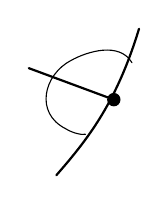
\begin{tikzpicture}[x=1cm,y=1cm,line cap=round]
\draw[thick] (.43,0) .. controls (.85,.48) and (1.20,.94) .. (1.48,1.86);
\draw (1.39,1.43) .. controls (1.23,1.70) and (.82,1.57) .. (.62,1.46)
 .. controls (.27,1.28) and (.15,.79) .. (.55,.59)
 .. controls (.63,.54) and (.74,.51) .. (.80,.52);
\draw[thick] (.08,1.36)--(1.16,.96);
\fill (1.16,.96) circle (.085);
\end{tikzpicture}}\endgroup
}
\end{GelfandAdjacentEvidence}
\begin{GelfandAdjacentEvidence}{GELFAND-P000997}{6}


or [crossed out: illegible] local rel. (?)

cell $\subset$ other cell.
\Unclear{GELFAND-P000997}{geometric-cancelled}{The word after “or” is crossed out.}
\end{GelfandAdjacentEvidence}
\begin{GelfandAdjacentEvidence}{GELFAND-P000997}{7}

\Unclear{GELFAND-P000997}{geometric-note}{Tentative reading “local relative”, with the first word abbreviated.}
\end{GelfandAdjacentEvidence}
\begin{GelfandAdjacentEvidence}{GELFAND-P000997}{8}


\underline{Zelevinsky.}\quad\underline{Other problems, the same polynoms.}
\SourceFigure{GELFAND-P000997}{zelevinsky-heading}{In the heading “the same” is followed by the abbreviation for “polynomials”.}
\end{GelfandAdjacentEvidence}
\begin{GelfandAdjacentEvidence}{GELFAND-P000997}{9}


Consider a finite-dimensional irreduc. rep.
\[
L(\chi)=\bigoplus_\lambda L(\chi)_\lambda.
\]
[Below $L(\chi)_\lambda$, joined by a stroke:] weight space with weight $\chi$.
\SourceFigure{GELFAND-P000997}{weight-annotation}{The label ends with the letter $\chi$.}
\end{GelfandAdjacentEvidence}
\begin{GelfandAdjacentEvidence}{GELFAND-P000997}{10}


\underline{I. M. G.} A good fn. for $\dim L(\chi)_\lambda$ is known
\[
\begin{vmatrix}
x_1^{a_1}&x_2^{a_1}&\ldots&x_n^{a_1}\\
x_1^{a_2}&x_2^{a_2}&\ldots&x_n^{a_2}\\
x_1^{a_n}&x_2^{a_n}&\ldots&x_n^{a_n}
\end{vmatrix}
:
\begin{vmatrix}
1&\ldots&1\\
x_1&\ldots&x_n\\
x_1^{n-1}&\ldots&x_n^{n-1}
\end{vmatrix}
=\sum m(\chi,\lambda)x^\lambda.
\]
\Unclear{GELFAND-P000997}{determinant-exponent}{The first exponent of $x_2$ reads as $a_1$ through the overlapping strokes.}
\end{GelfandAdjacentEvidence}



\Needspace{7\baselineskip}
\begin{GelfandAdjacentEvidence}{GELFAND-P000998}{1}
\SourcePage{GELFAND-P000998}{47}
Here
\[
\chi=(a_1,\ldots,a_n),\quad \lambda=(\lambda_1,\ldots,\lambda_n),
\qquad x^\lambda=x_1^{\lambda_1}\ldots x_n^{\lambda_n}.
\]
\[
m(\chi,\lambda)=\dim L(\chi)_\lambda.
\]

\underline{\underline{Problem}} (for first-year students).

Calculate
\[
\det\left\|\frac{1}{\lambda_i-\mu_j}\right\|_{i,j=1}^{n},
\qquad \lambda_i\ne\mu_j.
\]
[A star to the right of the matrix.]
\SourceFigure{GELFAND-P000998}{cauchy-difference}{The denominator is $\lambda_i-\mu_j$. A star is written to the right of the double bar.}
\end{GelfandAdjacentEvidence}
\begin{GelfandAdjacentEvidence}{GELFAND-P000998}{2}


\begin{center}$-\ \cdot\ -$\end{center}

\underline{Zelevinsky.}

[Crossed out before the formula: illegible.]
\[
m(\lambda,\chi)=P_{n_\lambda,n_\chi}(1).
\]
[Strokes from both indices lead to the label:] elements of the aff. Weyl gr.
\Unclear{GELFAND-P000998}{affine-cancelled-word}{The word before the formula is crossed out with dense strokes.}
\end{GelfandAdjacentEvidence}
\begin{GelfandAdjacentEvidence}{GELFAND-P000998}{3}

\Unclear{GELFAND-P000998}{affine-elements}{The indices of $P$ tentatively read $n_\lambda,n_\chi$.}
\end{GelfandAdjacentEvidence}
\begin{GelfandAdjacentEvidence}{GELFAND-P000998}{4}


\underline{Conjecture.}

The same $\forall$ Kac--Moody algebras.

[The entire formula is crossed out.]
\[
\operatorname{ch}L_\lambda(K_\mu)=P_{\lambda,\mu}(q).
\]
\Unclear{GELFAND-P000998}{cancelled-character}{The argument reads $K_\mu$ through the cancellation.}
\end{GelfandAdjacentEvidence}
\begin{GelfandAdjacentEvidence}{GELFAND-P000998}{5}


\underline{Elashvili.}

$G$ --- a lin. alg. group, i.e. $G\subset GL(n,\mathbb C)$.

$L(G)$ --- its Lie algebra.

$U(L)$ --- the universal enveloping alg.

$U(L)$ is called \underline{primitive} if the zero ideal is primitive ($=$ the kernel of an irreduc. rep.), i.e. there is a faithful [added above the line: (irreduc.)] rep. of $U(L)$.
\SourceFigure{GELFAND-P000998}{primitive-insertion}{“(irreduc.)” is inserted above “faithful rep.” with a bracket.}
\end{GelfandAdjacentEvidence}
\begin{GelfandAdjacentEvidence}{GELFAND-P000998}{6}


What conditions must $G$ and $L(G)$ satisfy? (question of \underline{Jacobson})

[Below the name:] last year.

Semisimple ones all [crossed out: unipotent (?)] [added above the line: (and nilpotent ones)] are unsuitable.
\Unclear{GELFAND-P000998}{excluded-cancelled}{The crossed-out word tentatively reads “unipotent”. Above it, a bracket contains “and nilpotent ones”.}
\end{GelfandAdjacentEvidence}
\begin{GelfandAdjacentEvidence}{GELFAND-P000998}{7}


\underline{Example:} 1) Lie alg. of the group of affine transf. ($L(G)$ consists of matr. with last column zero).
\SourceFigure{GELFAND-P000998}{zero-column}{The manuscript specifies the last column as zero.}
\end{GelfandAdjacentEvidence}
\begin{GelfandAdjacentEvidence}{GELFAND-P000998}{8}


2) $L=gl(2,\mathbb C)+V_4$.

[Below $V_4$, joined by a stroke:] commut. ideal.

$gl(2,\mathbb C)$ acts on $V_4$ by the unique $4$-dim. irreduc. rep.

[At right after two vertical strokes:] Another interesting $\Gamma$-fn. arises here.
\SourceFigure{GELFAND-P000998}{gamma-note}{The right-hand note reads “$\Gamma$-fn.”.}
\end{GelfandAdjacentEvidence}
\begin{GelfandAdjacentEvidence}{GELFAND-P000998}{9}


\underline{Thm.} There are no others if $L=R+V$, $R$ is [crossed out: illegible] simple, $V$ is commut., and the action of $R$ on $V$ is irreduc.
\Unclear{GELFAND-P000998}{theorem-cancelled}{The word after $R$ and before “simple” is crossed out with dense strokes.}
\end{GelfandAdjacentEvidence}


[Below the sum:] semidirect sum.

There is a method of construction beyond this.


\Needspace{7\baselineskip}
\begin{GelfandAdjacentEvidence}{GELFAND-P000999}{1}
\SourcePage{GELFAND-P000999}{unlabelled}
\underline{\underline{30/XI-81}}\quad\underline{Gelfand Sem.}

\underline{I. M. G.} On \underline{Reeb}'s talk at the Bourbaki sem. (November 1981)
[Below the date:] Cartier's survey.
\SourceFigure{GELFAND-P000999}{reeb-heading}{The talk line names Reeb. Below the date is “Cartier's survey”.}
\end{GelfandAdjacentEvidence}


\begin{equation*}
\varepsilon\ddot x+(x^2-1)\dot x+x=0.
\tag{1}
\end{equation*}
(Van der Pol)

What happens as $\varepsilon\to0$?


\begin{GelfandAdjacentEvidence}{GELFAND-P000999}{2}
\underline{$\varepsilon=0$:}
\[
\frac{dx}{dt}=-\frac{x}{x^2-1},\qquad
\frac{dx(1-x^2)}{x}=dt,\qquad
\frac{dx}{x}-x\,dx=dt.
\]
\[
C+t=\ln|x|-\frac{x^2}{2},\qquad
-\frac{x^2}{2}+\ln|x|=t+C.
\]
\SourceFigure{GELFAND-P000999}{solution-graphs}{The left plot has axes $t$ and $x$. The right plot has axes $x$ and $t$. Each plot has three branches on either side of the axis. Two lower branches at right have strokes resembling leftward arrows.\par\smallskip
\begingroup\color{black}\GelfandFitDiagram{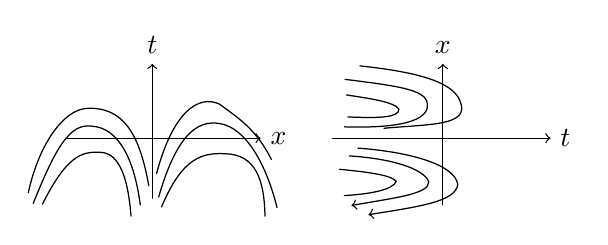
\begin{tikzpicture}[x=.90cm,y=.90cm,line cap=round,line width=.45pt]
\draw[->] (-1.20,0)--(1.53,0) node[right] {$x$};
\draw[->] (0,-.85)--(0,1.05) node[above] {$t$};
\draw (-1.75,-.77) .. controls (-1.60,-.08) and (-1.25,.40) .. (-.93,.42)
 .. controls (-.41,.45) and (-.18,.06) .. (-.05,-.67);
\draw (-1.68,-.92) .. controls (-1.36,-.12) and (-1.16,.21) .. (-.86,.17)
 .. controls (-.46,.15) and (-.25,-.33) .. (-.17,-.94);
\draw (-1.55,-.93) .. controls (-1.22,-.28) and (-1.02,-.18) .. (-.73,-.20)
 .. controls (-.45,-.21) and (-.34,-.60) .. (-.30,-1.10);
\draw (.06,-.50) .. controls (.29,.37) and (.65,.62) .. (.95,.48)
 .. controls (1.20,.29) and (1.46,.14) .. (1.68,-.30);
\draw (.09,-.83) .. controls (.36,.11) and (.68,.29) .. (1.02,.19)
 .. controls (1.39,.07) and (1.64,-.49) .. (1.76,-.98);
\draw (.13,-.97) .. controls (.42,-.28) and (.70,-.20) .. (1.03,-.22)
 .. controls (1.45,-.23) and (1.58,-.57) .. (1.59,-1.10);
\begin{scope}[shift={(4.1,0)}]
\draw[->] (-1.56,0)--(1.52,0) node[right] {$t$};
\draw[->] (0,-.94)--(0,1.05) node[above] {$x$};
\draw (-1.17,1.02) .. controls (-.42,.94) and (.13,.81) .. (.24,.53)
 .. controls (.40,.17) and (-.18,.20) .. (-.83,.14);
\draw (-1.38,.83) .. controls (-.67,.74) and (-.24,.69) .. (-.22,.49)
 .. controls (-.19,.31) and (-.42,.13) .. (-1.39,.16);
\draw (-1.36,.61) .. controls (-1.03,.56) and (-.68,.51) .. (-.62,.41)
 .. controls (-.62,.29) and (-.89,.28) .. (-1.34,.30);
\draw[->] (-1.20,-.14) .. controls (-.40,-.20) and (.17,-.39) .. (.21,-.65)
 .. controls (.19,-.90) and (-.37,-.97) .. (-1.05,-1.08);
\draw[->] (-1.32,-.25) .. controls (-.71,-.29) and (-.28,-.43) .. (-.20,-.61)
 .. controls (-.18,-.79) and (-.68,-.84) .. (-1.29,-.95);
\draw (-1.46,-.44) .. controls (-1.01,-.48) and (-.71,-.53) .. (-.66,-.61)
 .. controls (-.70,-.73) and (-1.04,-.79) .. (-1.39,-.81);
\end{scope}
\end{tikzpicture}}\endgroup
}
\end{GelfandAdjacentEvidence}
\begin{GelfandAdjacentEvidence}{GELFAND-P000999}{3}


Another remarkable eq.:
\begin{equation*}
\varepsilon\ddot u+\left(\frac{\dot u^3}{3}-\dot u\right)+u=0.
\tag{2}
\end{equation*}
(Rayleigh)

It reduces to the Van der Pol eq.

\SourceFigure{GELFAND-P000999}{jump-sketches}{Two curves with vertical segments. At the lower left endpoint is a downward arrow. The short stroke near the upper bend at right is unclear.\par\smallskip
\begingroup\color{black}\GelfandFitDiagram{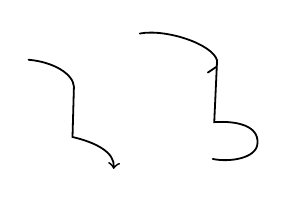
\begin{tikzpicture}[x=.9cm,y=.9cm,line cap=round,line width=.65pt]
\draw[->] (0,1.64) .. controls (.35,1.61) and (.63,1.44) .. (.64,1.26)
 --(.62,.55) .. controls (.96,.47) and (1.22,.33) .. (1.20,.10);
\draw (1.57,2.01) .. controls (1.94,2.08) and (2.60,1.86) .. (2.66,1.63)
 --(2.62,.76) .. controls (2.94,.78) and (3.25,.71) .. (3.23,.46)
 .. controls (3.22,.25) and (2.84,.19) .. (2.60,.24);
\draw (2.65,1.54)--(2.53,1.46);
\end{tikzpicture}}\endgroup
}
\end{GelfandAdjacentEvidence}
\begin{GelfandAdjacentEvidence}{GELFAND-P000999}{4}

[At right, with an arrow pointing left:] there are limiting solns. with such jumps.
\SourceFigure{GELFAND-P000999}{jump-caption}{The arrow from the label points toward the two curves.}
\end{GelfandAdjacentEvidence}
\begin{GelfandAdjacentEvidence}{GELFAND-P000999}{5}


Eq. (1) is studied using nonstandard analysis!

$\Omega$ --- a set,
\[
F=2^\Omega,\qquad p:F\to(0,1).
\]
\SourceFigure{GELFAND-P000999}{probability-codomain}{The interval is written with round brackets: $(0,1)$.}
\end{GelfandAdjacentEvidence}
\begin{GelfandAdjacentEvidence}{GELFAND-P000999}{6}

\[
p(A\cup B)=p(A)+p(B)\quad\text{when }A\cap B=\varnothing.
\]
$X$ --- a set,
\[
x':\Omega\to X,\qquad x'':\Omega\to X.
\]
A random element of $X$ is a class of equivalent maps $\Omega\to X$.

[In small writing below the line:]
\[
x'\sim x''\Leftrightarrow P(x'=x'')=1.
\]
\SourceFigure{GELFAND-P000999}{equivalence-probability-symbol}{The equivalence condition uses a capital $P$.}
\end{GelfandAdjacentEvidence}


[At right:] $x$ is the equiv. class of $x'$. $\Rightarrow x'$ is a version of $x$.


\Needspace{7\baselineskip}
\begin{GelfandAdjacentEvidence}{GELFAND-P001000}{1}
\SourcePage{GELFAND-P001000}{unlabelled}
\underline{Kruskal's numbers:} the simplest example of a field extending $\mathbb R$.
\SourceFigure{GELFAND-P001000}{surreal-heading}{The heading reads “Kruskal's”.}
\end{GelfandAdjacentEvidence}

\[
\varnothing=0.
\]
\[
\begin{aligned}
\text{up}\quad&\uparrow=1,\\
\text{down}\quad&\downarrow=-1,\\
&\overbrace{\uparrow\uparrow\uparrow\ldots\uparrow}^{n}=n,\\
&\uparrow\downarrow=\frac12,\\
&\uparrow\downarrow\uparrow=\frac34.
\end{aligned}
\]

\begin{GelfandAdjacentEvidence}{GELFAND-P001000}{2}
(when the direction changes the step is halved)
\SourceFigure{GELFAND-P001000}{halving-rule}{The manuscript says the step is halved when the direction changes.}
\end{GelfandAdjacentEvidence}
\begin{GelfandAdjacentEvidence}{GELFAND-P001000}{3}


$\hat{\uparrow}$ --- infinite repetition of $\uparrow$.
\[
\hat{\uparrow}\downarrow=\infty-1;\qquad
\hat{\uparrow}=\infty.
\]
[A sign before $\infty-1$ is crossed out.]
\Unclear{GELFAND-P001000}{infinity-cancelled-symbol}{Strokes to the left of $\infty$ obscure the crossed-out sign.}
\end{GelfandAdjacentEvidence}
\begin{GelfandAdjacentEvidence}{GELFAND-P001000}{4}

(there is no predecessor)
\begin{gather*}
\hat{\uparrow}\hat{\downarrow}=\frac12\infty.\\
\hat{\uparrow}:\hat{\uparrow}\hat{\downarrow}=2
\qquad\text{--- exact thm.}\\
\hat{\hat{\uparrow}}=\infty^2,\\
\uparrow\hat{\downarrow}=\varepsilon.
\end{gather*}
\SourceFigure{GELFAND-P001000}{iteration-hats}{In the last pair of formulas the first arrow has two arcs and the downward arrow has one.}
\end{GelfandAdjacentEvidence}
\begin{GelfandAdjacentEvidence}{GELFAND-P001000}{5}


\underline{Krichever.}

([Crossed out: illegible] from (?) work by Brozovskii, Dzyaloshinskii and Krichever)
\Unclear{GELFAND-P001000}{krichever-intro-cancelled}{A short entry is crossed out at the start of the parenthesis.}
\end{GelfandAdjacentEvidence}
\begin{GelfandAdjacentEvidence}{GELFAND-P001000}{6}

\Unclear{GELFAND-P001000}{intro-preposition}{The preposition between the cancellation and “work” tentatively reads «по».}
\end{GelfandAdjacentEvidence}
\begin{GelfandAdjacentEvidence}{GELFAND-P001000}{7}

\SourceFigure{GELFAND-P001000}{first-collaborator}{The surname is written «Брозовского», with «о» in the first syllable.}
\end{GelfandAdjacentEvidence}
\begin{GelfandAdjacentEvidence}{GELFAND-P001000}{8}

\[
G=\bigcup_n G_n,\qquad G_n\subset G_{n+1}.
\]
\Unclear{GELFAND-P001000}{group-chain-tail}{A short entry follows $G_{n+1}$. Its reading is unresolved.}
\end{GelfandAdjacentEvidence}
\begin{GelfandAdjacentEvidence}{GELFAND-P001000}{9}

\[
u(z),\qquad \Gamma\ni z.
\]
[Below $u(z)$, joined by a stroke:] matrix fn.
 
[Below $\Gamma$, joined by a stroke:] torus ($\mathbb C$/lattice).
\begin{gather*}
u^{ij}(z)=
\frac{\sigma(z-a_1^{ij})\ldots\sigma(z-a_n^{ij})}
{\sigma^n(z)}\,e^{\zeta(z)(x_i-x_j)},\\
a_1^{ij}+\ldots+a_n^{ij}=x_i-x_j.
\end{gather*}
\SourceFigure{GELFAND-P001000}{elliptic-exponent}{The exponent reads $\zeta(z)(x_i-x_j)$.}
\end{GelfandAdjacentEvidence}



\clearpage
\pdfbookmark[0]{Chapter 21}{gelfand-archive-chapter-21}
\section*{Chapter 21}
\Needspace{7\baselineskip}
\begin{GelfandAdjacentEvidence}{GELFAND-P001001}{1}
\SourcePage{GELFAND-P001001}{unlabelled}
\begin{center}$-\ \cdot\ -$\end{center}
\underline{\underline{8/II-82}}\qquad\underline{Gelfand Sem.}.

\underline{\underline{Müller Werner}}.

\underline{Lattice gravity}. (work with Cheeger and Schräder)
\SourceFigure{GELFAND-P001001}{collaborator-spelling}{The manuscript spells the name “Schräder”.}
\end{GelfandAdjacentEvidence}
\begin{GelfandAdjacentEvidence}{GELFAND-P001001}{2}


1) Consider a one-dim. mech. system with Hamiltonian:
\begin{equation*}
H(p,q)=+\frac{p^2}{2m}+V(q)
\tag{1}
\end{equation*}
\[
q\to Q,\quad p\to P\qquad \text{operators on }L^2(\mathbb R)
\]
\[
Qf(x)=xf(x),\qquad Pf(x)=i\hbar\frac{d}{dx}f(x)
\]
\SourceFigure{GELFAND-P001001}{momentum-sign}{There is no minus sign before $i\hbar$ in the expression for $Pf(x)$.}
\end{GelfandAdjacentEvidence}
\begin{GelfandAdjacentEvidence}{GELFAND-P001001}{3}

\[
H(p,q)\to\widehat H
\]
Consider Schrödinger's eq.
\begin{equation*}
i\frac{\partial}{\partial t}=\hbar^{-1}\widehat H f
\tag{2}
\end{equation*}
giving the evolution:
\begin{equation*}
f(x,t)=e^{-i\frac{t}{\hbar}\widehat H}f(x,0)
\tag{3}
\end{equation*}
\SourceFigure{GELFAND-P001001}{equation-two}{On the left of (2) the manuscript has only $i\,\partial/\partial t$. The letter $f$ is on the right.}
\end{GelfandAdjacentEvidence}
\begin{GelfandAdjacentEvidence}{GELFAND-P001001}{4}


Prob. of transition from $x$ to $x'$ in time [added above the line: from $t_0$ to] $t$, according to Feynman
\SourceFigure{GELFAND-P001001}{time-insertion}{The words “from $t_0$ to” are inserted before $t$.}
\end{GelfandAdjacentEvidence}
\begin{GelfandAdjacentEvidence}{GELFAND-P001001}{5}

\begin{equation*}
\langle x'\mid e^{-i\frac{t}{\hbar}\widehat H}\mid x\rangle
=\int_{\substack{\text{over [inserted: all] paths }x\\x(0)=x,\ x(t)=x'}}
e^{-iS[x]}\prod_\tau\frac{dx(\tau)}{2\pi}
\tag{4}
\end{equation*}
\SourceFigure{GELFAND-P001001}{path-insertion}{The word “all” is inserted above “over paths”.}
\end{GelfandAdjacentEvidence}
\begin{GelfandAdjacentEvidence}{GELFAND-P001001}{6}

\begin{equation*}
S[x]=\int_0^t[\dot x^2(\tau)-V(x(\tau))]d\tau
\tag{5}
\end{equation*}
\SourceFigure{GELFAND-P001001}{action-normalization}{The exponent in (4) is $-iS[x]$. In (5) there is no written coefficient before $\dot x^2(\tau)$.}
\end{GelfandAdjacentEvidence}
\begin{GelfandAdjacentEvidence}{GELFAND-P001001}{7}

(see last chapter of the book by Konopleva and Popov)
\Unclear{GELFAND-P001001}{bibliography}{The Russian surname reads «Коноплевой», with no distinct dots above the «е».}
\end{GelfandAdjacentEvidence}



\Needspace{7\baselineskip}
\begin{GelfandAdjacentEvidence}{GELFAND-P001002}{1}
\SourcePage{GELFAND-P001002}{4}
or: insert $t-t_0$ in place of $t$

\hspace{2em}in place of $0$ --- ditto --- $t_0$

\underline{M. Kac} gave some meaning to int. (4) with the substitution $i\to1$
\begin{equation*}
\hbar\frac{\partial f}{\partial t}=\widehat H f,
\tag{6}
\end{equation*}
then
\begin{equation*}
\langle x'\mid e^{-\frac{t}{\hbar}Hx}\mid x\rangle
=\int_{\substack{\text{over all paths}\\x:\,x(0)=x\\x(t)=x'}}
e^{-\int_0^t x(\tau)d\tau}\,dW(x)
\tag{7}
\end{equation*}
[Arrow to $dW(x)$:] Wiener measure.
\Unclear{GELFAND-P001002}{semigroup-exponent}{The letter $x$ follows $H$. Its status as a subscript is unclear.}
\end{GelfandAdjacentEvidence}
\begin{GelfandAdjacentEvidence}{GELFAND-P001002}{2}

\SourceFigure{GELFAND-P001002}{heat-kernel}{In (6) there is no minus sign before $\widehat Hf$ on the right.}
\end{GelfandAdjacentEvidence}
\begin{GelfandAdjacentEvidence}{GELFAND-P001002}{3}

\SourceFigure{GELFAND-P001002}{heat-integrand}{The integrand in the exponent reads $x(\tau)$.}
\end{GelfandAdjacentEvidence}
\begin{GelfandAdjacentEvidence}{GELFAND-P001002}{4}


2) \underline{Gravity}.
\[
i\mapsto1\qquad\rightsquigarrow
\]
[Crossed out: “for” (?)] Lorentz. metric $\longmapsto$ Riemannian metric.
\Unclear{GELFAND-P001002}{lorentz-cancellation}{The crossed-out word before “Lorentz.” tentatively reads “for”.}
\end{GelfandAdjacentEvidence}
\begin{GelfandAdjacentEvidence}{GELFAND-P001002}{5}


$M$ --- a compact $C^\infty$ manifold
\[
\mathcal M=\{\text{space of all Riem. metrics on }M\}
\]
\[
G=\operatorname{Diff}(M)\quad\text{--- gauge group.}
\]
Action [crossed out: illegible] [added below: Hilbert (-- Einstein)]:
\begin{equation*}
S[g]=\lambda\int_M R\,d\operatorname{vol},\qquad
R\text{ --- scalar curvature}
\tag{8}
\end{equation*}
\Unclear{GELFAND-P001002}{action-cancellation}{The earlier entry after “Action” is crossed out. Below it is “Hilbert (-- Einstein)”.}
\end{GelfandAdjacentEvidence}
\begin{GelfandAdjacentEvidence}{GELFAND-P001002}{6}


(nontrivial: Einstein thought there was no action)

--- $R$ contains 2nd derivs. $\Rightarrow$ \underline{a priori} a 4th-order eq.
\SourceFigure{GELFAND-P001002}{equation-order}{The end of the line reads “4th order”.}
\end{GelfandAdjacentEvidence}
\begin{GelfandAdjacentEvidence}{GELFAND-P001002}{7}


But locally there is a \underline{noncovar. addition} of divergence form, [crossed out: illegible] leaving $S$ unchanged.
\Unclear{GELFAND-P001002}{divergence-cancellation}{The reading under the cancellation after “form” is unresolved.}
\end{GelfandAdjacentEvidence}
\begin{GelfandAdjacentEvidence}{GELFAND-P001002}{8}


\underline{Problem (I.M.G.)} Find all comb. of curvatures yielding a lower-order eq.

\underline{“Answer”}: Einstein and Pontryagin classes. \underline{Action}:
\begin{equation*}
\int_{\mathcal M/G}e^{-S[g]-\text{æ}\operatorname{Vol}(M,g)}d\mu(g)
\tag{9}
\end{equation*}
\Unclear{GELFAND-P001002}{volume-coefficient}{The coefficient before $\operatorname{Vol}(M,g)$ resembles “æ”, possibly a handwritten $\varkappa$.}
\end{GelfandAdjacentEvidence}
\begin{GelfandAdjacentEvidence}{GELFAND-P001002}{9}


\underline{Formally}:
\begin{equation*}
d\mu(g)=\prod_{x\in M}\det g(x)^{5/2}\prod_{\mu\leq\nu}dg_{\mu\nu}(x)
\tag{10}
\end{equation*}
\SourceFigure{GELFAND-P001002}{measure-exponent}{The exponent reads $5/2$, with no minus sign.}
\end{GelfandAdjacentEvidence}
\begin{GelfandAdjacentEvidence}{GELFAND-P001002}{10}

(Faddeev -- Popov)

Lattice approximation.

[A number is crossed out at left.]
\[
P^n\subset\mathbb R^N\qquad
P^n\underset{\varphi}{\longrightarrow}M\quad\text{triangulation}
\]
[Stroke from $P^n$ to the label:] piecewise linear subset.
\Unclear{GELFAND-P001002}{bottom-cancellation}{Tentative reading of the crossed-out entry “(11)”.}
\end{GelfandAdjacentEvidence}



\Needspace{7\baselineskip}
\begin{GelfandAdjacentEvidence}{GELFAND-P001003}{1}
\SourcePage{GELFAND-P001003}{unlabelled}
The metric on $M$ induces a piecewise-lin. metr. on $P$.
\[
(P,\ell),\qquad \ell:P^{(1)}\to\mathbb R_+
\]
(simpl. $\rightsquigarrow$ its length)

(11)
\SourceFigure{GELFAND-P001003}{polyhedron-sphere}{Labels $P$, $\sigma^1$, $\varphi$ and $M=S^2$. The dashed strokes follow the visible portions.\par\smallskip
\begingroup\color{black}\GelfandFitDiagram{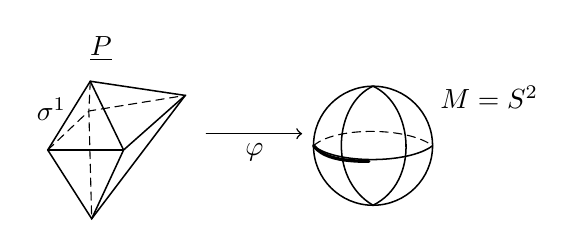
\begin{tikzpicture}[x=.9cm,y=.9cm,line cap=round,line width=.55pt]
\coordinate (top) at (.78,1.81);
\coordinate (west) at (.18,.84);
\coordinate (front) at (1.25,.84);
\coordinate (east) at (2.12,1.61);
\coordinate (low) at (.80,-.13);
\coordinate (rear) at (.76,1.39);
\draw[densely dashed,thin] (west)--(rear)--(east) (top)--(rear)--(low);
\draw (west)--(top)--(east)--(low)--cycle;
\draw (top)--(front)--(low) (west)--(front)--(east);
\node[above] at (.93,1.95) {\underline{$P$}};
\node[left] at (.58,1.41) {$\sigma^1$};
\draw[->] (2.42,1.07)--(3.77,1.07) node[midway,below] {$\varphi$};
\begin{scope}[shift={(4.77,.90)}]
\draw (0,0) circle (.84);
\draw (0,.84) .. controls (-.54,.60) and (-.65,-.46) .. (0,-.84);
\draw (0,.84) .. controls (.57,.58) and (.67,-.51) .. (0,-.84);
\draw[densely dashed,thin] (-.84,0) .. controls (-.54,.27) and (.48,.27) .. (.84,0);
\draw (-.84,0) .. controls (-.53,-.26) and (.50,-.26) .. (.84,0);
\draw[very thick] (-.84,0) .. controls (-.72,-.15) and (-.49,-.22) .. (-.06,-.22);
\node[right] at (.81,.69) {$M=S^2$};
\end{scope}
\end{tikzpicture}}\endgroup
}
\end{GelfandAdjacentEvidence}
\begin{GelfandAdjacentEvidence}{GELFAND-P001003}{2}


\underline{Discr. version of $\displaystyle\int_M R\,d\operatorname{vol}$}.
\begin{equation*}
P^n\longrightarrow M\qquad\text{triangulation}
\tag{12}
\end{equation*}
\[
\sigma^{n-2}\subset P^n
\]
$\delta(\sigma^{n-2})$ --- angle defect of $\sigma^{n-2}$
\[
\sigma^n\supset\sigma^{n-2}
\]
$[\sigma^{n-2},\sigma^n]$ --- dihedral angle
\begin{equation*}
\delta(\sigma^{n-2})=2\pi-\sum_{\sigma^n\supset\sigma^{n-2}}[\sigma^{n-2},\sigma^n]
\tag{13}
\end{equation*}
\begin{equation*}
R(P)=\sum_{\sigma^{n-2}\subset P}\delta(\sigma^{n-2})\operatorname{vol}(\sigma^{n-2})
\tag{14}
\end{equation*}
(Regge)

$P_n$ --- a seq. of triangulations, $P_n\to M$
\begin{equation*}
\operatorname{mesh}(P_n)\underset{n\to\infty}{\longrightarrow}0
\tag{15}
\end{equation*}
\begin{equation*}
\underline{\text{Th.}}\quad\underline{\text{Then}}\quad
R(P_n)\underset{n\to\infty}{\longrightarrow}\int_M R\,d\operatorname{vol}
\tag{16}
\end{equation*}
It is still unclear whether the eqs. converge.

Barycentric subdivision is unnecessary.
[Upward arrow to a note:] angles become small.
\SourceFigure{GELFAND-P001003}{skinny-simplex}{The interior strokes follow the visible joins. Some of the lower lines overlap.\par\smallskip
\begingroup\color{black}\GelfandFitDiagram{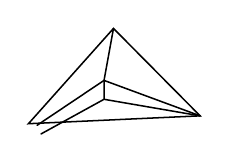
\begin{tikzpicture}[x=1cm,y=1cm,line cap=round,line width=.55pt]
\draw (0,0)--(1.08,1.21)--(2.18,.10)--cycle;
\draw (1.08,1.21)--(.96,.55)--(.96,.31);
\draw (.96,.55)--(.11,-.02) (.96,.55)--(2.18,.10);
\draw (.96,.31)--(.16,-.13) (.96,.31)--(2.18,.10);
\end{tikzpicture}}\endgroup
}
\end{GelfandAdjacentEvidence}
\begin{GelfandAdjacentEvidence}{GELFAND-P001003}{3}


\underline{The angles must be bounded away from $0$}:
\SourceFigure{GELFAND-P001003}{midpoint-subdivision}{The marks at the vertices are reproduced as strokes. It is unclear whether they are letters.\par\smallskip
\begingroup\color{black}\GelfandFitDiagram{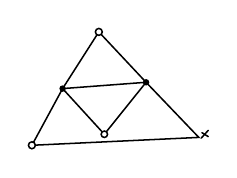
\begin{tikzpicture}[x=1cm,y=1cm,line cap=round,line width=.55pt]
\coordinate (a) at (0,0);
\coordinate (b) at (.85,1.44);
\coordinate (c) at (2.12,.10);
\coordinate (ab) at (.39,.72);
\coordinate (bc) at (1.45,.80);
\coordinate (ac) at (.92,.14);
\draw (a)--(ab)--(b)--(bc)--(c)--cycle;
\draw (ab)--(bc)--(ac)--cycle;
\draw[fill=white] (a) circle (.044) (b) circle (.044) (ac) circle (.041);
\fill (ab) circle (.041) (bc) circle (.041);
\draw (c) ++(.03,-.01)--++(.09,.10);
\draw (c) ++(.04,.06)--++(.08,-.05);
\end{tikzpicture}}\endgroup
}
\end{GelfandAdjacentEvidence}
\begin{GelfandAdjacentEvidence}{GELFAND-P001003}{4}

\underline{a smooth triangulation is taken}. (exists in Müller's work on Ray--Singer torsion)

\begin{center}$-\ \cdot\ -$\end{center}
\begin{equation*}
\int\operatorname{tr}(\Omega^k),\qquad \Omega\text{ --- curvature tensor}
\tag{17}
\end{equation*}
[Below $\Omega$, with a stroke to it:] 2-form.
\[
\sigma^{n-2k}\subset P^n
\]
\begin{equation*}
\begin{aligned}
R_k(P^n)={}&\sum_{\sigma^{n-2k}\in P}\operatorname{vol}(\sigma^{n-2k})\,
\sum_{\sigma^{n-2k}\subset\sigma^{n-2\ell_1}\subset\cdots\subset\sigma^{n-2\ell_j}}
(-1)^j\\
&[\sigma^{n-2k},\sigma^{n-2\ell_1}]\ldots
[\sigma^{n-2\ell_{j-1}},\sigma^{n-2\ell_j}]
\end{aligned}
\tag{18}
\end{equation*}
[Slanted above (18), with an arrow down and left:] norm. (?)
\SourceFigure{GELFAND-P001003}{formula-eighteen}{The last pair of indices in the product reads $\ell_{j-1},\ell_j$.}
\end{GelfandAdjacentEvidence}
\begin{GelfandAdjacentEvidence}{GELFAND-P001003}{5}

\Unclear{GELFAND-P001003}{formula-note}{The note tentatively reads “norm.”, with indistinct initial strokes.}
\end{GelfandAdjacentEvidence}



\Needspace{7\baselineskip}
\begin{GelfandAdjacentEvidence}{GELFAND-P001004}{1}
\SourcePage{GELFAND-P001004}{5}
$[\sigma^i,\sigma^{ij}]$ --- [inserted above: \underline{normalized}] dihedral angle (solid)
[Arrow to “solid”:] normalized to $1$.
\Unclear{GELFAND-P001004}{angular-indices}{The second superscript reads $ij$, with a faint initial stroke.}
\end{GelfandAdjacentEvidence}
\begin{GelfandAdjacentEvidence}{GELFAND-P001004}{2}


\begin{equation*}
\underline{\text{Th.}}\quad R_k(P_n)\longrightarrow\int_M\operatorname{tr}(\Omega^k) \tag{19}
\end{equation*}
$\Omega$ --- 2-form with values in the alg. [crossed-out sign] of matrices (a matrix of 2-forms).
\Unclear{GELFAND-P001004}{omega-algebra}{Crossed-out sign, possibly $A$.}
\end{GelfandAdjacentEvidence}
\begin{GelfandAdjacentEvidence}{GELFAND-P001004}{3}

\begin{equation*}
\underline{k=n/2}\quad\Rightarrow\quad\text{we obtain:}\quad\int\operatorname{tr}\Omega^k=\chi(M).
\end{equation*}
\Unclear{GELFAND-P001004}{euler-trace}{The manuscript reads $\int\operatorname{tr}\Omega^k=\chi(M)$.}
\end{GelfandAdjacentEvidence}
\begin{GelfandAdjacentEvidence}{GELFAND-P001004}{4}

\begin{equation*}
\begin{aligned}
\chi(M)={}&\sum_{\sigma^0\subset\sigma^{2\ell_1}\subset\cdots\subset\sigma^{2\ell_j}}
(-1)^j[\sigma^0,\sigma^{2\ell_1}]\\
&\ldots[\sigma^{2\ell_{j-1}},\sigma^{2\ell_j}]
\end{aligned}\tag{20}
\end{equation*}
\Unclear{GELFAND-P001004}{euler-cancellation}{Illegible crossed-out sign after the first closing bracket.}
\end{GelfandAdjacentEvidence}
\begin{GelfandAdjacentEvidence}{GELFAND-P001004}{5}

There is something similar in a work by \underline{Brin}, presented at the seminar ca. 1946. It is unknown what it gives in the limit.

$\displaystyle\int_M\operatorname{tr}(\Omega^k)$ is def. as follows: multiply $\operatorname{tr}(\Omega^k)$ by the standard [crossed out: form?] form ([inserted above: inv.] polynomial in the curvature).
\Unclear{GELFAND-P001004}{standard-form-cancellation}{The crossed-out word tentatively reads “form.”}
\end{GelfandAdjacentEvidence}
\begin{GelfandAdjacentEvidence}{GELFAND-P001004}{6}

\begin{equation*}
\mathcal M(P^n)=\{\text{space of all piecewise-lin. metrics on }P^n\}\tag{21}
\end{equation*}
$\sigma^n\subset\mathbb R^N$ \(\xrightarrow{\quad}\) $n$-dim. simplex

\SourceFigure{GELFAND-P001004}{tetrahedron}{Vertices $0,1,2,3$, with edge labels $\ell_{01}$ and $\ell_{03}$.\par\smallskip
\begingroup\color{black}\GelfandFitDiagram{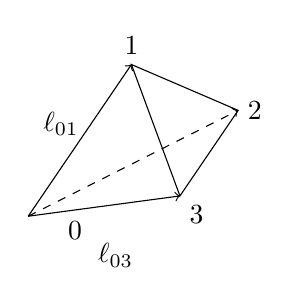
\begin{tikzpicture}[scale=1.12]
\coordinate (v0) at (0,0);
\coordinate (v1) at (1.17,1.72);
\coordinate (v2) at (2.38,1.2);
\coordinate (v3) at (1.72,0.23);
\draw[->] (v0) -- (v1);
\draw (v1) -- (v2) -- (v3) -- cycle;
\draw[->] (v0) -- (v3);
\draw[dashed,->] (v0) -- (v2);
\node[below] at (0.53,0.05) {$0$};
\node[above] at (v1) {$1$};
\node[right] at (v2) {$2$};
\node[below right] at (v3) {$3$};
\node[above left] at (0.68,0.8) {$\ell_{01}$};
\node[below] at (0.99,-0.2) {$\ell_{03}$};
\end{tikzpicture}}\endgroup
}
\end{GelfandAdjacentEvidence}
\begin{GelfandAdjacentEvidence}{GELFAND-P001004}{7}


\[
\ell\rightsquigarrow g=(g_{ij}),\qquad
g_{ij}=\frac12(\ell_{0i}^2+\ell_{0j}^2-\ell_{ij}^2)
\]
\begin{flushright}\underline{symm. and positive definite}\end{flushright}
\[
\mathcal P=\{\text{symm. pos. def. matrices }n\times n\}
\]
'' $GL(n)/O(n)$
\[
\mathcal M(\sigma^n)\equiv GL(n)/O(n)
\]
\underline{Inv. measure on $\mathcal M(\sigma^n)$}:
\begin{equation*}
\frac{1}{\det g^{\frac{n+1}{2}}}\prod_{i\le j}dg_{ij}\tag{22}
\end{equation*}
\begin{equation*}
\frac{1}{\operatorname{vol}(\sigma^n,\ell)^{n+1}}\prod d\ell_{ij}\tag{23}
\end{equation*}
--- measure on $\mathcal M(\sigma^n)$ (another way of writing it).
\Unclear{GELFAND-P001004}{measure-change}{In (23) the manuscript gives $\prod d\ell_{ij}$.}
\end{GelfandAdjacentEvidence}
\begin{GelfandAdjacentEvidence}{GELFAND-P001004}{8}

\begin{equation*}
\prod_{x\in M}\operatorname{deg}g(x)^{5/2}\prod_{\mu\le\nu}dg_{\mu\nu}\tag{24}
\end{equation*}
\Unclear{GELFAND-P001004}{last-measure}{The final stroke of “deg” descends below the line, unlike “det” in (22). The exponent in (24) is written as $5/2$.}
\end{GelfandAdjacentEvidence}



\Needspace{7\baselineskip}
\begin{GelfandAdjacentEvidence}{GELFAND-P001005}{1}
\SourcePage{GELFAND-P001005}{unlabelled}
\begin{equation*}
\mathcal M(P^n)\hookrightarrow\prod_{\sigma^n\subset P^n}\mathcal M(\sigma^n) \tag{25}
\end{equation*}
(sub-set)

An induced [crossed out on the line: metric?] [circled and crossed out above: curvature?] [circled below: metric] arises on $\mathcal M(P^n)$ [crossed out on the right: not satisfy…].
\Unclear{GELFAND-P001005}{metric-cancel-main}{On the line, tentatively “metric,” with most of the word crossed out.}
\end{GelfandAdjacentEvidence}
\begin{GelfandAdjacentEvidence}{GELFAND-P001005}{2}

\Unclear{GELFAND-P001005}{metric-cancel-upper}{The circled and crossed-out word above the line may read “curvature” or “metric.”}
\end{GelfandAdjacentEvidence}
\begin{GelfandAdjacentEvidence}{GELFAND-P001005}{3}

\Unclear{GELFAND-P001005}{right-cancellation}{Under the cancellation, “not satisfy…” is legible. The ending and following strokes remain unclear.}
\end{GelfandAdjacentEvidence}


($\rightsquigarrow$ gluing cond.)

A measure is introduced on the space of all metrizations. $\Rightarrow$ volume induced by the Riem. metric.
\[
P_n\underset{n\to\infty}{\longrightarrow}M
\]
(On $\mathcal M(\sigma^n)$ the inv. metric is the one on a symmetric space.)

\underline{Idea}: $M^n\subset E^N$ \underline{isometric.}

Chern’s kinematic formula:
\[
k=N-n+2,
\]
$\mathcal G_{N,k}$ = affine Grassmannian of $E^k\subset E^N$

$dE^k$ --- measure on $\mathcal G_{N,k}$
\begin{equation*}
\int_{E^k\in\mathcal G_{N,k}}\chi(M^n\cap E^k)\,dE^k
=c_{N,k}\int_M R\,d\operatorname{vol} \tag{26}
\end{equation*}
\begin{equation*}
\int_{\mathcal G_{N,k}}\chi(P^n\cap E^k)\,dE^k
=c_{N,k}R(P^n) \tag{27}
\end{equation*}
[Under $P^n$, with a vertical stroke:] simplicial sub-set

[Below the right-hand side:] (combinat. scalar curvature)
\[
P_n\longrightarrow M
\]
the integrands in (26) and (27) will agree a.e.

\begin{GelfandAdjacentEvidence}{GELFAND-P001005}{4}
\begin{center}--- . ---\end{center}
For $\displaystyle\int\operatorname{tr}(\Omega^k)$, $k=N-n+2\ell$
\begin{equation*}
\int_{E^k\in\mathcal G_{N,k}}\chi(M^n\cap E^k)\,dE^k
=c_{N,k}\int_M\operatorname{tr}(\Omega^\ell) \tag{28}
\end{equation*}
\Unclear{GELFAND-P001005}{curvature-exponent}{The line before (28) reads $\Omega^k$, and the right-hand side of (28) reads $\Omega^\ell$.}
\end{GelfandAdjacentEvidence}

\begin{equation*}
\underset{\text{left-hand side of (27)}}{\text{--- '' ---}}=c_{N,k}R_\ell(P^n). \tag{29}
\end{equation*}


\Needspace{7\baselineskip}
\begin{GelfandAdjacentEvidence}{GELFAND-P001006}{1}
\SourcePage{GELFAND-P001006}{6}
\underline{15/II-82}\qquad \underline{Gelfand Sem.}

\underline{Ginzburg.}

$M$ --- sympl. manifold

($\omega$ --- corresp. 2-form)

$A$ --- group acting on $M$ in a Hamiltonian way.

1) $A$ preserves $\omega$

$\xi\in\mathfrak A$ --- corresp. Lie algebra

$\xi\longrightarrow\omega(\xi,\cdot)$ globally (?) exact; exact:
\Unclear{GELFAND-P001006}{exactness-word}{The word before “exact” tentatively reads “globally,” with a tall medial loop. “Locally” is also possible.}
\end{GelfandAdjacentEvidence}
\begin{GelfandAdjacentEvidence}{GELFAND-P001006}{2}


2) $\mathfrak A\ni a\longmapsto H_a$\quad (Hamiltonian)

homomorphism of Lie algebras.

\underline{moment map}: $\mu\colon M\longrightarrow\mathfrak A^*$
\[
m\longmapsto\mu(m),\qquad
\mu(m)(\underset{\substack{\uparrow\\\mathfrak A}}{a})=H_a(m)
\]
\SourceFigure{GELFAND-P001006}{moment-map-argument}{The arrow from $\mathfrak A$ below points to the argument $a$.}
\end{GelfandAdjacentEvidence}


Commutes with the action of $A$ and is compat. with the Poisson bracket.

\begin{flushright}[Two short slanted strokes.]\end{flushright}


\Needspace{7\baselineskip}
\begin{GelfandAdjacentEvidence}{GELFAND-P001007}{1}
\SourcePage{GELFAND-P001007}{unlabelled}
\underline{22/II-82}\qquad \underline{Gelfand Sem.}

\underline{Arnold.}

\[
V(\varepsilon)=\sum_{i=0}^{n}V_k\varepsilon^k,\qquad
\sigma_i(k)=\sum_{C_n^i}k_1\ldots k_i
\]
[Under $V(\varepsilon)$:] volume ($\varepsilon$-neighborhood of a conv. body). \quad (Minkowski’s theorem --- this is a polynomial.)
\Unclear{GELFAND-P001007}{summation-index}{The summation starts at $i=0$, while the summand reads $V_k\varepsilon^k$.}
\end{GelfandAdjacentEvidence}
\begin{GelfandAdjacentEvidence}{GELFAND-P001007}{2}


\[
k_s\text{ --- eigenvalues of }\frac{2\ \text{quadr. f.}}{1\ \text{quadr. f.}}
\]
\[
V_i=C_i\int_{\partial D}\sigma_i(k)\,dS
\]
[Short vertical stroke below $C_i$.]
\[
V_k=\widetilde C_k
\underbrace{\int_{\xi\in G_{n,k}}\operatorname{mes}(\pi_\xi D)\,d\xi}_{\text{''}},
\qquad \pi_\xi\colon \mathbb R^n\longrightarrow\xi
\]
\[
\int_{H_{n,k}}\chi(h\cap D)\,dh
\]
\SourceFigure{GELFAND-P001007}{integral-link}{A bracket with turned-up ends and two short slanting strokes appear below the upper integral.}
\end{GelfandAdjacentEvidence}
\begin{GelfandAdjacentEvidence}{GELFAND-P001007}{3}


$H_{n,k}$ --- all planes, not necessarily passing through $0$

$\chi$ --- Euler char..

\underline{This is the method of} [crossed out: Buff\ldots] \underline{Buffon} (later generalized by Santaló)
[Below “method of Buffon”:] for computing the number $\pi$.
\Unclear{GELFAND-P001007}{buffon-cancellation}{The first strokes, “Buff\ldots”, are visible under the cancellation.}
\end{GelfandAdjacentEvidence}
\begin{GelfandAdjacentEvidence}{GELFAND-P001007}{4}


Computation of the constants $C_k$, $\widetilde C_k$ --- using balls.

\underline{This carries over to the lattice case.}

In place of volume, the number of integer points.

\underline{integral parallelogram} (\ldots piped?)
\Unclear{GELFAND-P001007}{parallelogram-caption}{The letters after the dots tentatively read “piped.”}
\end{GelfandAdjacentEvidence}
\begin{GelfandAdjacentEvidence}{GELFAND-P001007}{5}


\SourceFigure{GELFAND-P001007}{parallelogram-diagram}{The lower edge continues as a dashed line. A loop at the lower right vertex may be a separate $0$.\par\smallskip
\begingroup\color{black}\GelfandFitDiagram{\begin{tikzpicture}[x=.75cm,y=.75cm,line width=.45pt]
\coordinate (a) at (0,0);
\coordinate (b) at (1.8,.9);
\coordinate (c) at (2.72,2.73);
\coordinate (d) at (.92,1.83);
\draw (a)--(b)--(c)--(d)--cycle;
\draw[dashed] (-1.42,-.71)--(a) (b)--(3.8,1.9);
\fill (a) circle (1.5pt) (b) circle (1.5pt)
      (c) circle (1.5pt) (d) circle (1.5pt);
\draw (1.76,.91) to[out=220,in=230] (1.81,.79) to[out=50,in=275] (1.86,.92);
\end{tikzpicture}}\endgroup
}
\end{GelfandAdjacentEvidence}
\begin{GelfandAdjacentEvidence}{GELFAND-P001007}{6}


The volume of a parallelepiped is the number showing how many elem. par.-pipeds there are.

A lattice of intersections arises on the line.

Take the quotient space and this gives an analogue of height.

(there is an analogue of a lattice there too)

\underline{Mac Mullen} a talk in [crossed out: Vancou\ldots] Vancouver --- there are refs. there.
\Unclear{GELFAND-P001007}{vancouver-cancellation}{The first spelling is crossed out. The beginning reads “Vancou\ldots”.}
\end{GelfandAdjacentEvidence}
\begin{GelfandAdjacentEvidence}{GELFAND-P001007}{7}


\underline{I. M. Gelfand.}

\underline{On Mc Donald’s book} “Symmetric Functions and Hall Polynomials”

\underline{Problem.} Consider a partition (partition)
\[
(L)\qquad \lambda_1\geq\lambda_2\geq\ldots\geq\lambda_k
\qquad (\text{integers})
\]
Adding zeros is allowed.

Ways of writing it: $(L)$ or
\[
\begin{array}{rccccc}
5&\bullet&\bullet&\bullet&\bullet&\bullet\\
4&\bullet&\bullet&\bullet&\bullet&\\
4&\bullet&\bullet&\bullet&\bullet&\\
1&\bullet&&&&
\end{array}
\]
Squares are better than dots (Young diagrams).

\SourceFigure{GELFAND-P001007}{young-diagram}{Rows of $5,4,4,1$ cells in a dashed frame marked $m$ and $n$.\par\smallskip
\begingroup\color{black}\GelfandFitDiagram{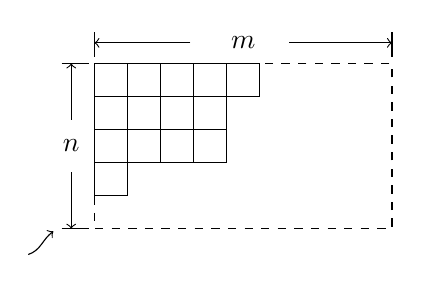
\begin{tikzpicture}[x=.42cm,y=.42cm,line width=.4pt]
\draw[dashed] (0,0) rectangle (9,-5);
\draw (0,0)--(5,0)--(5,-1)--(4,-1)--(4,-3)--(1,-3)--(1,-4)--(0,-4)--cycle;
\draw (0,-1)--(4,-1) (0,-2)--(4,-2) (0,-3)--(1,-3);
\draw (1,0)--(1,-3) (2,0)--(2,-3) (3,0)--(3,-3) (4,0)--(4,-1);
\draw (0,.2)--(0,.96) (9,.2)--(9,.96);
\draw[->] (2.9,.62)--(0,.62);
\draw[->] (5.9,.62)--(9,.62);
\node at (4.5,.62) {$m$};
\draw (-.99,0)--(-.15,0) (-.99,-5)--(-.15,-5);
\draw[->] (-.7,-1.7)--(-.7,0);
\draw[->] (-.7,-3.3)--(-.7,-5);
\node at (-.7,-2.5) {$n$};
\draw[->] (-2,-5.78) to[out=18,in=216] (-1.24,-5.08);
\end{tikzpicture}}\endgroup
}
\end{GelfandAdjacentEvidence}


Place it in a rectangle of dimensions $m\times n$ and consider the numbers


\Needspace{7\baselineskip}
\begin{GelfandAdjacentEvidence}{GELFAND-P001008}{1}
\SourcePage{GELFAND-P001008}{11}
\[
(*)\quad\left\{
\begin{array}{ll}
\lambda_i+n-i,&1\leq i\leq n,\\
n-1+j-\lambda'_j,&1\leq j\leq m
\end{array}\right.
\]

$\lambda'=4,3,3,3,1$ --- dual diagram

\underline{Problem:}

The list of $m+n$ numbers $(*)$ --- is a permutation of the numbers $0,1,2,\ldots,m+n-1$.

\underline{Corollary.}
\[
f_{\lambda,n}(t)\overset{\mathrm{def}}{=}\sum_{i=1}^{n}t^{\lambda_i+n-i}
\]
Then
\[
f_{\lambda,n}(t)+t^{m+n-1}f_{\lambda,m}(t)=\frac{1-t^{m+n}}{1-t}
\]
\Unclear{GELFAND-P001008}{generating-function}{The second term reads $f_{\lambda,m}(t)$, with no visible prime on $\lambda$ and no inverse argument.}
\end{GelfandAdjacentEvidence}
\begin{GelfandAdjacentEvidence}{GELFAND-P001008}{2}


\underline{I. M. Gelfand} from the work of \underline{Guillemin}
\Unclear{GELFAND-P001008}{author-name}{The manuscript surname tentatively reads “Гийемина” (Guillemin).}
\end{GelfandAdjacentEvidence}
\begin{GelfandAdjacentEvidence}{GELFAND-P001008}{3}


\underline{New cond. for Weyl’s asympt. formula}

\underline{Sympl. cone:}\qquad $\rho_a^*\omega=a\omega$,\quad $a>0$.

\underline{Example 1.} $\mathbb R^{2n}=\{(x,\xi)\}$,
$x\in\mathbb R^n$, $\xi\in(\mathbb R^n)^*$,
$\rho_a(x,\xi)=(a^{1/2}x,a^{1/2}\xi)$.

\underline{Example 2.} $T^*X$\qquad $a(x,\xi)=(x,a\xi)$.
\Unclear{GELFAND-P001008}{cotangent-base}{The base after $T^*$ is heavily overwritten and tentatively reads $X$.}
\end{GelfandAdjacentEvidence}
\begin{GelfandAdjacentEvidence}{GELFAND-P001008}{4}


\underline{Arnold.}

Locally all cones are the same: the quotient is a contact manifold.

(Sympl. cones $\Longleftrightarrow$ contact manifolds)

The quantization must be contact quantization, since we need the action --- \underline{a 1-form!!}
\Unclear{GELFAND-P001008}{contact-ending}{The ending of the word following “must be” tentatively gives the singular “contact.”}
\end{GelfandAdjacentEvidence}
\begin{GelfandAdjacentEvidence}{GELFAND-P001008}{5}


\underline{Claim.} Can always be quantized and the Weyl alg. is constr. uniquely, microlocally unique, and topol. (microlocally) classical Weyl alg.
\Unclear{GELFAND-P001008}{construction-abbreviation}{The abbreviation before “Weyl alg.” reads “стр.” (constr.).}
\end{GelfandAdjacentEvidence}
\begin{GelfandAdjacentEvidence}{GELFAND-P001008}{6}


\underline{Quantization} --- [crossed out: a set\ldots]
\Unclear{GELFAND-P001008}{quantization-cancellation}{The beginning of the crossed-out line reads “a set\ldots”.}
\end{GelfandAdjacentEvidence}
\begin{GelfandAdjacentEvidence}{GELFAND-P001008}{7}


\[
x_k\longmapsto x_k,\qquad \xi_k\longmapsto i\frac{\partial}{\partial x_k}.
\]
\Unclear{GELFAND-P001008}{quantization-convention}{The image of $\xi_k$ contains $i$ with no minus sign.}
\end{GelfandAdjacentEvidence}
\begin{GelfandAdjacentEvidence}{GELFAND-P001008}{8}

\[
p(x,\xi)=\sum_{i=0}^{\infty}p_i(x,\xi),\qquad
p_i\text{ --- homog. of degree }2\mu-2i
\]
\[
\rho_a(x,\xi)=(a^{1/2}x,a^{1/2}\xi);\qquad \mu\in\mathbb C.
\]
(This is a symbol of order $\mu$).
\[
(Pf)(x)=(2\pi)^{-n}\int p\left(\frac{x+y}{2},\xi\right)
  e^{i\xi\cdot(x-y)}u(y)\,dy\,d\xi
\]
\Unclear{GELFAND-P001008}{kernel-function}{The left-hand side reads $(Pf)(x)$ and the integrand uses $u(y)$.}
\end{GelfandAdjacentEvidence}
\begin{GelfandAdjacentEvidence}{GELFAND-P001008}{9}


$W^\mu$ --- space of such operators,\qquad $\underline{W^{\mu-1}\subset W^\mu}$.

\underline{Symbol:} element of $W^\mu/W^{\mu-1}$.

$H$ --- Hilbert space, $S$ --- dense subspace on which all such op. act.

$\underline W^\mu$ --- corresp. space of op.
(of the form $A_1+\cdots+A_k$, $A_i\in W^{\mu_i}$ in the example).
\Unclear{GELFAND-P001008}{w-subscript}{Below $W$ are crossed-out looped strokes. The subscript reading is unresolved.}
\end{GelfandAdjacentEvidence}


\underline{Axioms:}
\[
\substack{\text{group}\\ A}
\quad\left\lceil
\begin{aligned}
1)\quad &\underline W^\mu\supset\underline W^{\mu-1}\\
2)\quad &A\in\underline W^\mu,\quad B\in\underline W^\nu
 \ \Longrightarrow\ AB\in\underline W^{\mu+\nu}\\
3)\quad &A\in\underline W^\mu,\quad B\in\underline W^\nu
 \ \Longrightarrow\ [A,B]\in\underline W^{\mu+\nu-1}\\
4)\quad &A\in\underline W^\mu\ \Longrightarrow\ A^*\in\underline W^{\bar\mu}
\end{aligned}\right.
\]
\[
5)\quad I\in\underline W^0
\]


\Needspace{7\baselineskip}
\begin{GelfandAdjacentEvidence}{GELFAND-P001009}{1}
\SourcePage{GELFAND-P001009}{unlabelled}
\[
\left\lfloor
\begin{aligned}
6)\quad&\forall A_i\in\underline W^{\mu-i},\quad i=0,1,2,\ldots\\
&\Longrightarrow\ \exists A\in\underline W^\mu,\qquad
A-\sum_{i=0}^{N-1}A_i\in\underline W^{\mu-N}.
\end{aligned}\right.
\]
\SourceFigure{GELFAND-P001009}{asymptotic-bracket}{To the left of item 6) is the lower end of a square bracket.}
\end{GelfandAdjacentEvidence}
\begin{GelfandAdjacentEvidence}{GELFAND-P001009}{2}


\underline{Group $B$.}

$1^{\circ}$. If $\operatorname{Re}\mu\leq0$, then $\forall A\in\underline W^\mu$ is bounded.

$2^{\circ}$. If $\operatorname{Re}\mu<0$, then $\forall A\in\underline W^\mu$ is compact.

$3^{\circ}$. $\exists s_0>0$, if $A\in\underline W^\mu$,
$\operatorname{Re}\mu<-s_0$; then $A$ is nuclear.

\underline{Group $C$.}
\[
A\in\underline W^0,\quad A\text{ is compact}
\ \Longrightarrow\ A\in\underline W^{-1}
\]

\underline{$D$.} Exact seq.

\SourceFigure{GELFAND-P001009}{exact-sequence}{Underlines on $W$ and arrows of the sequence.\par\smallskip
\begingroup\color{black}\GelfandFitDiagram{\begin{tikzcd}[ampersand replacement=\&,column sep=small]
0\arrow[r]\&\underline W^{\mu-1}\arrow[r]\&\underline W^\mu\arrow[r]\&
\underline W^\mu/\underline W^{\mu-1}\arrow[r]\&0
\end{tikzcd}}\endgroup
}
\end{GelfandAdjacentEvidence}


“Nicely” decomp. into a direct sum.

\underline{$E$.}\qquad $\exists A(\mu)\in\underline W^\mu$, depending analyt. on $\mu\in\mathbb C$,
such that $A(0)-I\in\underline W^{-1}$ and
\[
A(\mu)A(\nu)-A(\nu+\mu)\in\underline W^{\mu+\nu-1}.
\]


\Needspace{7\baselineskip}
\begin{GelfandAdjacentEvidence}{GELFAND-P001010}{1}
\SourcePage{GELFAND-P001010}{15}
\underline{\underline{1/III-82.}}\qquad \underline{Gelfand Sem.}

\underline{R. MacPherson.}\quad \underline{The title of a paper}
[crossed out: which?] \underline{he would speak about:}
\Unclear{GELFAND-P001010}{title-cancellation}{The crossed-out English word tentatively reads “which.”}
\end{GelfandAdjacentEvidence}
\begin{GelfandAdjacentEvidence}{GELFAND-P001010}{2}


\SourceFigure{GELFAND-P001010}{title-diagram}{“Holonomes” and “char variety” retain the manuscript spellings. The wavy and dashed arrows point toward the lower label.\par\smallskip
\begingroup\color{black}\GelfandFitDiagram{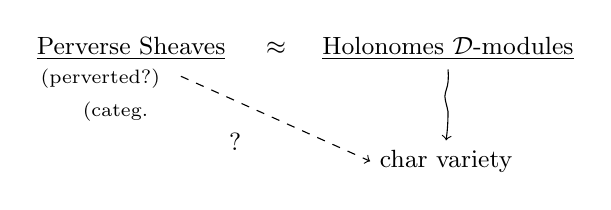
\begin{tikzpicture}[x=.80cm,y=.67cm,font=\small]
\node (p) at (0,0) {\underline{Perverse Sheaves}};
\node at (2.30,0) {$\approx$};
\node (h) at (5.03,0) {\underline{Holonomes $\mathcal D$-modules}};
\node[font=\scriptsize] at (-.49,-.58) {(perverted?)};
\node[font=\scriptsize] at (-.25,-1.20) {(categ.};
\node (v) at (5.0,-2.14) {char variety};
\draw[dashed,->] (.79,-.53)--(v.west);
\node at (1.65,-1.77) {?};
\draw[->] (h.south) to[out=275,in=85] (5.03,-.64)
 to[out=265,in=85] (4.98,-.91) to[out=275,in=100] (5.03,-1.20)
 to[out=270,in=83] (v.north);
\end{tikzpicture}}\endgroup
}
\end{GelfandAdjacentEvidence}
\begin{GelfandAdjacentEvidence}{GELFAND-P001010}{3}


\underline{Another title:}

$H(X\longrightarrow Y)$\qquad \underline{homol. theory of maps of spaces.}
\begin{align*}
H(X\longrightarrow pt)&=H_*(X)\\
H(X\overset{\mathrm{id}}{\longrightarrow}X)&=H^*(X)
\end{align*}

\SourceFigure{GELFAND-P001010}{composition-diagram}{The lower arc points from $X$ to $Z$.\par\smallskip
\begingroup\color{black}\GelfandFitDiagram{\begin{tikzcd}[ampersand replacement=\&]
X\arrow[r]\arrow[rr,bend right=25]\&Y\arrow[r]\&Z
\end{tikzcd}}\endgroup
}

\underline{there is a product}, covering comp. of maps.
\end{GelfandAdjacentEvidence}
\begin{GelfandAdjacentEvidence}{GELFAND-P001010}{4}

\underline{D. McDuff.}\qquad \underline{Cohom. of the group of volume-preserving diffeom.}

\[
\mathcal G=\operatorname{Diff}_{\omega 0}^{c}M,
\]
$\omega$ --- volume form on $M$, $M$ --- a manifold;

$c$ --- with comp. support; $0$ --- connected component of $Id$.

$\mathcal G$ with the usual topology $(C^\infty)$.

$G$ --- the same group with the discr. top.
\[
G\underset{\text{ident.}}{\longrightarrow}\mathcal G
\]
\[
\bar B\mathcal G\longrightarrow
\overset{\substack{K(G,1)\\\shortparallel}}{BG}
\longrightarrow B\mathcal G
\qquad (\text{classifying spaces})
\]
\SourceFigure{GELFAND-P001010}{classifying-spaces}{Above $BG$ is $K(G,1)$ with two short strokes. A stroke from $\bar B\mathcal G$ leads to the fiber annotation.}
\end{GelfandAdjacentEvidence}
\begin{GelfandAdjacentEvidence}{GELFAND-P001010}{5}

homot. fiber (turn the map into a fibration, then $\bar B\mathcal G$ --- fiber)

$\bar B\mathcal G$ depends only on a neighb. of $1$ in $\mathcal G$.

This is a topological version of the Lie alg. in some sense.

\underline{Fuks:}
\[
G/H\longrightarrow BH\longrightarrow BG
\]
(usually); if $H$ is [inserted above: very] dense in $G$, then the fund. domain is an “infinitesim.” neighb. of the identity.

$\bar B\mathcal G\times M$ has a foliation $\mathcal F$,
transverse to all fibers $x\times M$
and defined by [inserted above: such] a closed $n$-form $\Omega$, that $\Omega|_{x\times M}=\omega$.
\Unclear{GELFAND-P001010}{closed-form-overwriting}{The end of “closed” has heavily overwritten strokes.}
\end{GelfandAdjacentEvidence}
\begin{GelfandAdjacentEvidence}{GELFAND-P001010}{6}


\SourceFigure{GELFAND-P001010}{bundle-diagram}{The lower left label reads $\bar BG$ and the upper left uses $\bar B\mathcal G$. The product sign at top runs into the strokes of $M$. An entry above the right-hand $M$ is heavily crossed out.\par\smallskip
\begingroup\color{black}\GelfandFitDiagram{\begin{tikzcd}[ampersand replacement=\&,column sep=small]
E'\cong\bar B\mathcal G\times M\arrow[d]\&E'\arrow[d,"M"]\&E\arrow[d,"M"]\\
\bar B G\arrow[r]\&BG\arrow[r]\&B\mathcal G
\end{tikzcd}}\endgroup
}
\end{GelfandAdjacentEvidence}
\begin{GelfandAdjacentEvidence}{GELFAND-P001010}{7}


$E$ --- std. bundle with fiber $M$.

$E'$ --- its lift, [crossed out: connection?] it has zero curvature,
since the fiber of the corresp. principal bundle is discrete.
\Unclear{GELFAND-P001010}{connection-cancellation}{The crossed-out word has an initial “с” and tentatively reads “connection.”}
\end{GelfandAdjacentEvidence}


On the left, the restriction to the fiber becomes triv. by the property of the classifying space.

The zero-curvature connection is transferred and gives a foliation on $\bar B\mathcal G\times M$


\Needspace{7\baselineskip}
\begin{GelfandAdjacentEvidence}{GELFAND-P001011}{1}
\SourcePage{GELFAND-P001011}{unlabelled}
$\Omega-\pi^*\omega=0$ near $\infty$ on $M$.

Classes.
\[
c_k(M)\in H^k\left(\bar B\operatorname{Diff}^{c}_{\omega_0}M;
\underset{\substack{\vert\\\text{coefficients}}}{H_c^{n-k}(M;\mathbb R)}\right)
\]
$n=\dim M$.

Let $K$ --- $k$-cycle in $\bar B\operatorname{Diff}^{k}_{\omega_0}M$.
\Unclear{GELFAND-P001011}{upper-diff-superscript}{In the definition of the cycle the superscript on $\operatorname{Diff}$ is $k$. The neighboring formulas use $c$.}
\end{GelfandAdjacentEvidence}
\begin{GelfandAdjacentEvidence}{GELFAND-P001011}{2}

\[
c_k(M)(K)=\text{class of the closed }(n-k)\text{-form }
 x\longmapsto\int_{K\times x}\Omega
\]

\underline{Example.} $M=T^n$, $K=T^n$.
\[
\begin{aligned}
T^n\times T^n&\longrightarrow T^n\\
(x,y)&\longmapsto x+y
\end{aligned}
\]
Take [crossed out: a foliation on $T^n$ and lift it?] [inserted above in a callout: a foliation arises]
on $T^n\times T^n$. Obtain a foliation repr. a cycle in $\bar B\operatorname{Diff}^{c}_{\omega_0}T^n$.
\Unclear{GELFAND-P001011}{middle-cancelled-verb}{The crossed-out verb means “lift.” Its tense is uncertain.}
\end{GelfandAdjacentEvidence}
\begin{GelfandAdjacentEvidence}{GELFAND-P001011}{3}

\[
c_n(T^n)(T^n)=\int_{T^n\times x}\Omega
\qquad\text{indep. of the choice of }x.
\]

\underline{Prop.} 1
\[
\begin{aligned}
c_n(S^n)&=0\quad\text{for }n\text{ even}\\
&\ne0\quad\text{for }n\text{ odd}
\end{aligned}
\]
\underline{1st claim:}
$K^n\times S^n$\qquad ($K^n$ --- any manifold)

$\Omega$ --- form defining a foliation transv. to the spheres.
\SourceFigure{GELFAND-P001011}{foliation-diagram}{Six nearly vertical strokes, a transverse straight line and a curve.\par\smallskip
\begingroup\color{black}\GelfandFitDiagram{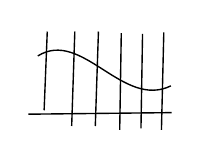
\begin{tikzpicture}[x=1cm,y=1cm,line width=.5pt]
\draw (0,0.05)--(0.04,1.05);
\draw (0.35,-0.15)--(0.39,1.05);
\draw (0.65,-0.15)--(0.69,1.05);
\draw (0.96,-0.2)--(0.98,1.03);
\draw (1.23,-0.18)--(1.25,1.02);
\draw (1.49,-0.2)--(1.52,1.04);
\draw (-0.2,0)--(1.62,0.02);
\draw (-0.08,.74)..controls (.48,1.09) and (1.00,.06)..(1.61,.36);
\end{tikzpicture}}\endgroup
}
\end{GelfandAdjacentEvidence}
\begin{GelfandAdjacentEvidence}{GELFAND-P001011}{4}

\[
\text{Then }\int_{\substack{\text{horiz.}\\\text{leaf}}}\Omega=0.
\]
Constr. another class $s$

\underline{Prop.} 2
\[
\begin{aligned}
s(\mathbb R^n)&\ne0\quad n\text{ even}\\
&=0\quad n\text{ odd}
\end{aligned}
\]

\underline{\underline{Milnor}}.

$G$ --- Lie group, $G^\delta$ --- the same with the discr. topology.
\[
\begin{gathered}
G^\delta\longrightarrow G\\
BG^\delta\longrightarrow BG
\end{gathered}
\]
\[
H_*\left(\qquad\begin{matrix}\mathbb Q\\\mathbb Z\\\mathbb Z_p\end{matrix}\right)\ -\ ?
\]
\Unclear{GELFAND-P001011}{milnor-coefficients}{The space to the left of the column $\mathbb Q,\mathbb Z,\mathbb Z_p$ in the parentheses is blank.}
\end{GelfandAdjacentEvidence}


$H_*(BG)$ are well known and well behaved

$H_*(BG^\delta)$ --- ?

are unknown and badly behaved. It is unclear whether they are useful.

In algebraic $K$-theory, in foliation theory, in Hilbert’s 3rd problem

--- all this comes up. \qquad (equidecomposability)


\Needspace{7\baselineskip}
\begin{GelfandAdjacentEvidence}{GELFAND-P001012}{1}
\SourcePage{GELFAND-P001012}{16}
\underline{Isomorphism conjecture:}
\[
(1)\qquad H_*(BG^\delta,\mathbb Z/p)\overset{\simeq}{\longrightarrow}
H_*(BG,\mathbb Z/p);\qquad \underline{\forall\ \text{prime }p.}
\]
Applied to Hilb.’s 3rd problem by H. Sah, Dupont.

When are they equidecomposable? A partial answer comes from the cohomology of the classifying space.

Probably (1) is a very difficult assertion.

\underline{Chern--Weyl:} $G$ compact $\Rightarrow$
\[
\widetilde H_*(BG^\delta,\mathbb Q)\overset{0}{\longrightarrow}
\widetilde H_*(BG,\mathbb Q).
\]
(the map is trivial)

\underline{Sah--Wagoner}:
\Unclear{GELFAND-P001012}{upper-sah-name}{The second surname reads “Wagoner.”}
\end{GelfandAdjacentEvidence}
\begin{GelfandAdjacentEvidence}{GELFAND-P001012}{2}

\[
\underset{\text{connected}}{G}\ne1
\quad\Rightarrow\quad\exists\ \text{an epimorphism}
\]
\[
H_2(BG^\delta,\mathbb Z)\longrightarrow
\underset{\substack{\text{uncount.}\\\text{sum}}}{\bigsqcup}\mathbb Q\longrightarrow0
\]
At the same time:
\par $H_2(BG,\mathbb Z)$ is finitely generated.

\underline{Let us discuss evid. for (1).}

\tikz[baseline=(n.base)]{\node[draw,circle,inner sep=1pt](n){1};}
(1) holds in the spec. case when the Lie alg. $\mathfrak g$ is solvable.

The proof is elementary.
\[
\bar B G\longrightarrow BG^\delta\longrightarrow BG
\]
[Below $\bar B G$ with a vertical stroke:] prove by ind. that the cohom. of $\bar B G$ is trivial.

\tikz[baseline=(n.base)]{\node[draw,circle,inner sep=1pt](n){2};}
Let $G$ have finitely many components.

Then (1) is an epim. and splits.
\[
H_*(BG^\delta,\mathbb Z/p)
\underset{\underline{\mathrm{split}}}{\longrightarrow}
H_*(BG,\mathbb Z/p)\longrightarrow0
\]
\Unclear{GELFAND-P001012}{middle-arrow-cancellation}{Short strokes above the arrow are crossed out, possibly “ep.”}
\end{GelfandAdjacentEvidence}
\begin{GelfandAdjacentEvidence}{GELFAND-P001012}{3}


[Crossed-out sign at left.] (2)\quad \underline{Corollary.}
\Unclear{GELFAND-P001012}{left-margin-cancelled-number}{The crossed-out looped sign to the left of (2) is unresolved.}
\end{GelfandAdjacentEvidence}
\begin{GelfandAdjacentEvidence}{GELFAND-P001012}{4}


\SourceFigure{GELFAND-P001012}{middle-cohomology-arrow}{Both heads are visible on the middle arrow. A bracket appears below the expression.\par\smallskip
\begingroup\color{black}\GelfandFitDiagram{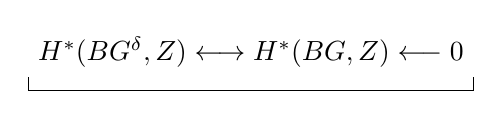
\begin{tikzpicture}
\node (seq) {$H^*(BG^\delta,\mathbb Z)\longleftrightarrow H^*(BG,\mathbb Z)\longleftarrow0$};
\draw (seq.south west) -- ++(0,-.17) -| (seq.south east);
\end{tikzpicture}}\endgroup
}
\end{GelfandAdjacentEvidence}
\begin{GelfandAdjacentEvidence}{GELFAND-P001012}{5}


Gen. --- thm. [crossed out: Du?] Bott--Heitsch.
\Unclear{GELFAND-P001012}{lower-bott-cancellation}{The cancellation before Bott--Heitsch may read “Du.”}
\end{GelfandAdjacentEvidence}
\begin{GelfandAdjacentEvidence}{GELFAND-P001012}{6}


\tikz[baseline=(n.base)]{\node[draw,circle,inner sep=1pt](n){3};}
(1) always holds [crossed out: when] for $H_1$ and in interesting cases for $H_2$:
\[
\operatorname{SL}_n\mathbb R,\quad \operatorname{SL}_n\mathbb C.
\]
\Unclear{GELFAND-P001012}{lower-sl-cancellation}{A sign below the line between the index $n$ and $\mathbb R$ is heavily crossed out, possibly $\mathbb Z$.}
\end{GelfandAdjacentEvidence}
\begin{GelfandAdjacentEvidence}{GELFAND-P001012}{7}


\underline{Haefliger.}

$\operatorname{PSL}_2(\mathbb Z)$ on $\operatorname{Im}z>0$.

(fractional-lin. transf. [crossed out: co?] with integral coeff.)
\Unclear{GELFAND-P001012}{lower-fractional-cancellation}{The crossed-out fragment may begin “co.”}
\end{GelfandAdjacentEvidence}
\begin{GelfandAdjacentEvidence}{GELFAND-P001012}{8}


\SourceFigure{GELFAND-P001012}{circle-boundary}{Circle and boundary label.\par\smallskip
\begingroup\color{black}\GelfandFitDiagram{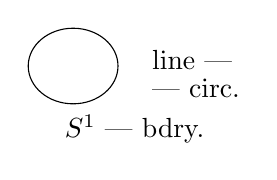
\begin{tikzpicture}[x=1cm,y=1cm]
\draw (0,0) ellipse (.57 and .48);
\node[anchor=west] at (.88,.08) {line ---};
\node[anchor=west] at (.88,-.28) {--- circ.};
\node[anchor=west] at (-.23,-.80) {$S^1$ --- bdry.};
\end{tikzpicture}}\endgroup
}
\end{GelfandAdjacentEvidence}
\begin{GelfandAdjacentEvidence}{GELFAND-P001012}{9}


$\gamma_1,\gamma_2$ --- \underline{generators}.
\[
\gamma_1:z\longmapsto z+1;\qquad
\gamma_2:z\longmapsto-\frac{1}{z}.
\]
$\forall f\in C^\infty(S^1),\quad\exists?\,C^\infty$-fns. $f_1,f_2\in C^\infty(S^1)$
\Unclear{GELFAND-P001012}{exists-question}{A question mark with a separate dot follows $\exists$.}
\end{GelfandAdjacentEvidence}



\Needspace{7\baselineskip}
\SourcePage{GELFAND-P001013}{unlabelled}
\[
(1)\qquad f(x)=f_1(x)-f_1(\gamma_1(x))+f_2(x)-f_2(\gamma_2(x)).
\]
This is related to foliations on a Riem. manifold whose leaves are \underline{min.} surfaces.

\underline{Unknown}!

Approximately true: approximation is possible ( in the $C^\infty$ top. ) --- this is easy.


\Needspace{7\baselineskip}
\begin{GelfandAdjacentEvidence}{GELFAND-P001014}{1}
\SourcePage{GELFAND-P001014}{unlabelled}
15/\underline{III}-82.\qquad \underline{Gelfand Sem.}

\underline{Topics} (for term papers, diploma theses, etc.)

\underline{Kirillov}:

\SourceFigure{GELFAND-P001014}{weight-branches}{The upper and lower strokes lead to two separate items.\par\smallskip
\begingroup\color{black}\GelfandFitDiagram{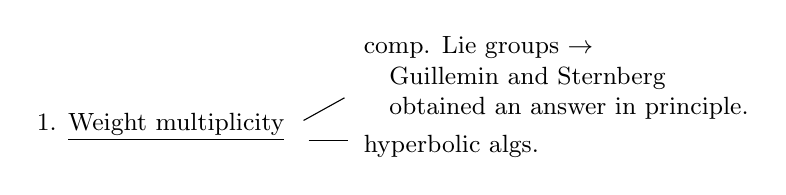
\begin{tikzpicture}[font=\small,x=.8cm,y=.8cm]
\node[anchor=east] at (0,0) {1. \underline{Weight multiplicity}};
\draw (.15,.11)--(.80,.47);
\draw (.23,-.21)--(.85,-.21);
\node[anchor=west,align=left] at (.95,.78) {comp. Lie groups $\to$\\\quad Guillemin and Sternberg\\\quad obtained an answer in principle.};
\node[anchor=west] at (.95,-.30) {hyperbolic algs.};
\end{tikzpicture}}\endgroup
}
\end{GelfandAdjacentEvidence}
\begin{GelfandAdjacentEvidence}{GELFAND-P001014}{2}

\SourceFigure{GELFAND-P001014}{weight-response}{The arrow after “comp. Lie groups” points to Guillemin and Sternberg.}
\end{GelfandAdjacentEvidence}


\underline{Refs.}: \underline{Macdonald} (article)

\underline{Example} \underline{problem} in \underline{2}: a contragredient Lie algebra with a hyperbolic Cartan matrix (having a neg. eigenvalue) is considered.

Consider the action of $SU(3)$ on its Lie algebra:
\[
X=\begin{pmatrix}
i\varphi_1&a&c\\
-\bar a&i\varphi_2&b\\
-\bar c&-\bar b&i\varphi_3
\end{pmatrix},\qquad
\varphi_1+\varphi_2+\varphi_3=0
\]
\[
g\in SU(3)\Rightarrow g:X\to gXg^*.
\]


\Needspace{7\baselineskip}
\begin{GelfandAdjacentEvidence}{GELFAND-P001015}{1}
\SourcePage{GELFAND-P001015}{unlabelled}
Consider the orbit $\Omega$. [separate stroke] It has the form:
\Unclear{GELFAND-P001015}{orbit-punctuation}{A separate slanted stroke follows the period. It could be $1$ or part of an exclamation mark.}
\end{GelfandAdjacentEvidence}
\begin{GelfandAdjacentEvidence}{GELFAND-P001015}{2}

\[
\begin{cases}
\operatorname{tr}\,\text{[crossed-out sign]}\,X^2=c_2,\\
\operatorname{tr}X^3=c_3
\end{cases}
\qquad (\text{and, incidentally, }\operatorname{tr}X=0)
\]
\Unclear{GELFAND-P001015}{trace-cancellation}{Between $\operatorname{tr}$ and $X^2$ is a heavily crossed-out sign.}
\end{GelfandAdjacentEvidence}
\begin{GelfandAdjacentEvidence}{GELFAND-P001015}{3}

(these traces recover the roots, and $\forall$ matr. can be brought into diag. form)

Denote it by $\Omega_{c_2,c_3}$.

The orbit is of dimension 6 (gen. position).

Project onto the plane (2-dim.) $(\varphi_1,\varphi_2,\varphi_3)$,
$\varphi_1+\varphi_2+\varphi_3=0$.

\SourceFigure{GELFAND-P001015}{diagonal-axes}{Three axes labelled $\varphi_1,\varphi_2,\varphi_3$ with three $120^\circ$ angles.\par\smallskip
\begingroup\color{black}\GelfandFitDiagram{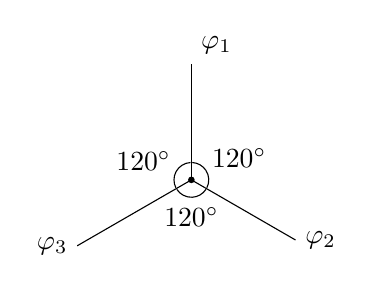
\begin{tikzpicture}[x=.92cm,y=.92cm]
\draw (0,0)--(0,1.6) node[above right] {$\varphi_1$};
\draw (0,0)--(-30:1.66) node[right] {$\varphi_2$};
\draw (0,0)--(210:1.82) node[left] {$\varphi_3$};
\fill (0,0) circle[radius=1.2pt];
\draw (93:.24) arc (93:207:.24);
\draw (213:.24) arc (213:327:.24);
\draw (333:.24) arc (333:447:.24);
\node at (-.66,.26) {$120^\circ$};
\node at (.66,.30) {$120^\circ$};
\node at (0,-.51) {$120^\circ$};
\end{tikzpicture}}\endgroup
}
\end{GelfandAdjacentEvidence}
\begin{GelfandAdjacentEvidence}{GELFAND-P001015}{4}


\SourceFigure{GELFAND-P001015}{cancelled-axes}{An upward arrow is visible in the crossed-out sketch. The underlying geometry and labels are unresolved.}
\end{GelfandAdjacentEvidence}
\begin{GelfandAdjacentEvidence}{GELFAND-P001015}{5}


--- project onto the plane $\varphi_1+\varphi_2+\varphi_3=0$
[crossed out: illegible] the coordinate axes.
\Unclear{GELFAND-P001015}{projection-cancellation}{A short entry before “coordinate axes” is crossed out.}
\end{GelfandAdjacentEvidence}
\begin{GelfandAdjacentEvidence}{GELFAND-P001015}{6}


--- this is how it should be drawn. \qquad ($p$ --- projection)

\underline{Facts}:

a) The projection of $\Omega_{c_1,c_2}$ fills a hexagon.
\Unclear{GELFAND-P001015}{orbit-indices}{The indices on this line are $c_1,c_2$. The designation above has $c_2,c_3$.}
\end{GelfandAdjacentEvidence}
\begin{GelfandAdjacentEvidence}{GELFAND-P001015}{7}


\SourceFigure{GELFAND-P001015}{orbit-hexagon}{Hexagon, three outgoing arrows and three dashed interior lines.\par\smallskip
\begingroup\color{black}\GelfandFitDiagram{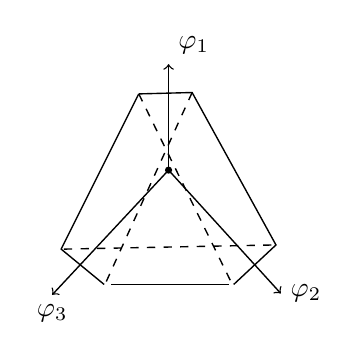
\begin{tikzpicture}[x=.88cm,y=.88cm,line width=.5pt]
\draw (-.43,1.33)--(.34,1.35)--(1.55,-.85)--(.94,-1.42);
\draw (.87,-1.42)--(-.83,-1.42);
\draw (-.93,-1.42)--(-1.55,-.91)--(-.43,1.33);
\draw[dashed] (-.43,1.33)--(.91,-1.40) (.34,1.35)--(-.90,-1.38)
(-1.51,-.91)--(1.52,-.85);
\draw[->] (0,.23)--(0,1.76) node[above right] {$\varphi_1$};
\draw[->] (0,.23)--(1.62,-1.55) node[right] {$\varphi_2$};
\draw[->] (0,.23)--(-1.68,-1.57) node[below] {$\varphi_3$};
\fill (0,.23) circle[radius=1.3pt];
\end{tikzpicture}}\endgroup
}
\end{GelfandAdjacentEvidence}
\begin{GelfandAdjacentEvidence}{GELFAND-P001015}{8}


(this is the set of diag. entries of matrices with fixed eigenvalues $\lambda_1,\lambda_2,\lambda_3$)

b) \underline{Consider} $p^{-1}(y_0)$, $y_0$ --- a point of the hexagon.

It is a 4-dimensional manifold. Regularity fails on the dashed lines.
\Unclear{GELFAND-P001015}{fibre-dimension}{A long thin vertical line crosses the horizontal stroke after $4$. “4-dimensional” is the probable reading.}
\end{GelfandAdjacentEvidence}
\begin{GelfandAdjacentEvidence}{GELFAND-P001015}{9}


This is all in the paper of \underline{Berezin} and \underline{Gelfand} in Tr. MMO, 1956. \quad (“Some remarks on the theory of spherical fns.”)

A rep. of $SU(3)$ is given by a \underline{pair of integers} and the weights follow from them.

The weights are inside the hexagon. Multiplicities:

\SourceFigure{GELFAND-P001015}{weight-contours}{Three nested hexagonal contours surround a hatched triangle. Overlapping strokes obscure some marks at the upper-left corner.\par\smallskip
\begingroup\color{black}\GelfandFitDiagram{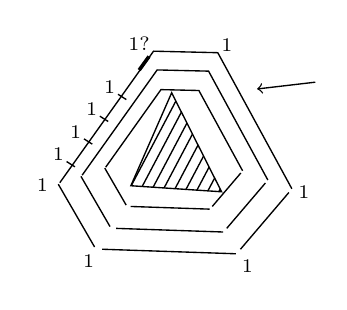
\begin{tikzpicture}[x=.96cm,y=.96cm,line width=.49pt]
\foreach \size in {1,.80,.59} {
  \begin{scope}[scale=\size]
    \draw (-1.48,-.50)--(-.24,1.24)--(.61,1.22)--(1.59,-.58);
    \draw (1.55,-.63)--(.91,-1.38);
    \draw (.85,-1.44)--(-.92,-1.38);
    \draw (-1.02,-1.35)--(-1.50,-.52);
  \end{scope}
}
\draw (0,.69)--(.66,-.62)--(-.54,-.54)--cycle;
\begin{scope}
\clip (0,.69)--(.66,-.62)--(-.54,-.54)--cycle;
\foreach \x in {-.78,-.63,-.48,-.33,-.18,-.03,.12,.27,.42,.57} {
  \draw (\x,-.72)--++(.77,1.46);
}
\end{scope}
\foreach \x/\y in {-1.71/-.54,-1.10/-1.54,1.00/-1.60,1.75/-.63,.73/1.32} {
  \node[font=\scriptsize] at (\x,\y) {$1$};
}
\foreach \x/\y in {-1.32/-.25,-1.09/.05,-.88/.35,-.64/.64} {
  \draw (\x-.07,\y+.03)--(\x+.04,\y-.04);
  \node[font=\scriptsize] at (\x-.18,\y+.12) {$1$};
}
\draw[line width=1.3pt] (-.43,.99)--(-.30,1.17);
\node[font=\scriptsize] at (-.43,1.34) {$1?$};
\draw[<-] (1.13,.74)--(1.90,.83);
\end{tikzpicture}}\endgroup
}
\end{GelfandAdjacentEvidence}
\begin{GelfandAdjacentEvidence}{GELFAND-P001015}{10}

$\leftarrow$ lines of changing multiplicity

$SU(3)$ --- in Gelfand and Berezin.

The answer of \underline{Guillemin, Sternberg} --- for large $c_2,c_3$.

[Above the names, with an arrow to them:] preprint $\approx\underline{1981\text{}}$

$X$ --- the preimage of \textsuperscript{*?} a point,
$X=p^{-1}(y_0)$.
\Unclear{GELFAND-P001015}{preimage-mark}{A star-like sign between “preimage” and “point” may be a crossed-out entry.}
\end{GelfandAdjacentEvidence}
\begin{GelfandAdjacentEvidence}{GELFAND-P001015}{11}


\[
\langle e^B\tau,X\rangle\quad\text{--- multiplicity!!}
\]
[Below $e^B$ the strokes of an equals sign are turned vertically.]
\[
e^B=1+B+\frac{B\wedge B}{2}+\ldots
\]
$B$ --- sympl. form on the orbit.

$\tau$ --- Todd class of the manifold.

\underline{I. M. G.}\qquad \underline{Main question}: duality between groups and their representations.
\[
x^{\text{\tikz[baseline=(n.base)]{\node[draw,circle,inner sep=0.3pt] (n) {$\scriptstyle n$};}}}
=x(x-1)\ldots(x-n+1)
\]
\[
\text{\tikz[baseline=(d.base)]{\node[draw,circle,inner sep=1pt] (d) {$\frac{d}{dx}$};}}f(x)
=f(x+1)-f(x)
\]
\SourceFigure{GELFAND-P001015}{circled-operators}{The circles around $n$ and $\frac{d}{dx}$ are part of the author's notation.}
\end{GelfandAdjacentEvidence}



\Needspace{7\baselineskip}
\begin{GelfandAdjacentEvidence}{GELFAND-P001016}{1}
\SourcePage{GELFAND-P001016}{25}
Then
\SourceFigure{GELFAND-P001016}{circled-falling-factorial}{%
\(\displaystyle
\text{\tikz[baseline=(d.base)]{\node[draw,circle,inner sep=1pt] (d) {$\frac{d}{dx}$};}}
x^{\text{\tikz[baseline=(n.base)]{\node[draw,circle,inner sep=.3pt] (n) {$\scriptstyle n$};}}}
=n\,x^{\text{\tikz[baseline=(m.base)]{\node[draw,ellipse,inner sep=.4pt] (m) {$\scriptstyle n-1$};}}}\)}
\end{GelfandAdjacentEvidence}
\begin{GelfandAdjacentEvidence}{GELFAND-P001016}{2}


\Unclear{GELFAND-P001016}{cancelled-heading}{A short entry is enclosed and crossed out. Its reading remains unresolved.}
\end{GelfandAdjacentEvidence}
\begin{GelfandAdjacentEvidence}{GELFAND-P001016}{3}


Dual: for a representation, look at the weight multiplicities.

There is a (unique) invariant volume on the orbit.

Normalization: volume of the \underline{orbit} $=$ \underline{dimension} of the linear representation associated with it.
\SourceFigure{GELFAND-P001016}{representation-abbreviation}{of the linear representation associated with it.}
\end{GelfandAdjacentEvidence}
\begin{GelfandAdjacentEvidence}{GELFAND-P001016}{4}


Jacobi polynomials
\[
\bigl(x^k(1-x)^\ell\bigr)^{(p)}=F(k,\ell,p;x)
=\int_0^x t^k(1-t)^\ell(x-t)^{-p-1}\,dt
\]
\Unclear{GELFAND-P001016}{fractional-normalization}{There is no prefactor between the equals sign and the integral.}
\end{GelfandAdjacentEvidence}
\begin{GelfandAdjacentEvidence}{GELFAND-P001016}{5}


All $k,\ell,p$ --- \underline{are nonintegers}\qquad (Gauss hypergeometric function)

\underline{Fractional derivative}:
\[
(x^n)^{(k)}=x^{n-k}\frac{n!}{(n-k)!}
\qquad\text{or}\qquad
\left(\frac{x^n}{n!}\right)^{(k)}=\frac{x^{n-k}}{(n-k)!}
\]
and replace $!$ by $\Gamma$.

There is no satisfactory theory of \underline{hypergeometric functions of several} variables (important for representations)

\underline{Atiyah}: generalization of the statement that the points $\in$ a convex polygon, to the case where only the Cartan group acts.

Idea: recast all of representation theory in terms of the action of the Cartan group.

\underline{References}: 1) Berezin, Gelfand\quad 2) Atiyah\quad
3) Guillemin, Sternberg\quad 4) Khovanskii

\SourceFigure{GELFAND-P001016}{newton-reference}{%
on Newton polyhedra\par
\(\swarrow\)\par
from polygons ---\par
--- multiplicity functions.\par
(and Kazarnovskii)}
\end{GelfandAdjacentEvidence}



\Needspace{7\baselineskip}
\begin{GelfandAdjacentEvidence}{GELFAND-P001017}{1}
\SourcePage{GELFAND-P001017}{46}
\underline{29/III/82}\qquad\underline{Gelfand seminar.}

\underline{Givental.}

\underline{Thm. 1.} $M$ --- a smooth manifold, $N$ --- a submanifold.

$\omega_0,\omega_1$ --- two symplectic structures on $M$
\[
\omega_0|_{TN}=\omega_1|_{TN}
\]
Then $\forall x\in N$, $\exists$ a neighbourhood $U$ and a diffeomorphism
$g:U\to U$, such that
\[
g|_N=\mathrm{id}_N,\qquad g^*\omega_1=\omega_0.
\]

\begin{center}--- $\cdot$ ---\end{center}
\underline{A. Weinstein} proved this if
$\omega_0|_{TM|_N}=\omega_1|_{TM|_N}$.
(he wrote $\omega_0|_N=\omega_1|_N$)

\begin{center}--- $\cdot$ ---\end{center}
\underline{Moral}: there is no extrinsic symplectic geometry for a submanifold.

\begin{center}--- $\cdot$ ---\end{center}
There are also global formulations.

\begin{center}--- $\cdot$ ---\end{center}
\underline{Idea of the proof}: take a family $g_t$, $\omega_t$
\Unclear{GELFAND-P001017}{proof-superscript}{Above $g_t$ a mark is crossed out, possibly an asterisk.}
\end{GelfandAdjacentEvidence}
\begin{GelfandAdjacentEvidence}{GELFAND-P001017}{2}


\SourceFigure{GELFAND-P001017}{proof-annotations}{%
\begin{tabular}{@{}cc@{}}
\(g_t\) & \(\omega_t\)\\
\(\vert\) & \(\diagdown\)\\
diffeomorphism & symplectic structure
\end{tabular}}
\end{GelfandAdjacentEvidence}
\begin{GelfandAdjacentEvidence}{GELFAND-P001017}{3}

\[
g_t^*\omega_t=\omega_0.
\]
Differentiate and then use the existence and uniqueness theorem for differential equations. (reduces to a linear problem)

$N=\{*\}$ $\Rightarrow$ a new proof of Darboux’s theorem.

[Question: under what conditions is a 2-form obtained by restricting a symplectic form.
\Unclear{GELFAND-P001017}{restriction-cancellation}{A short word is crossed out.}
\end{GelfandAdjacentEvidence}
\begin{GelfandAdjacentEvidence}{GELFAND-P001017}{4}

necessary condition: $d\omega=0$].

\underline{I. M. G.} There is no need to add a closedness condition yet:
a symplectic structure in $\forall$ tangent space.

A symplectic form has no properties.

\begin{center}--- $\cdot$ ---\end{center}
\underline{Symplectic structure in the space of polynomials.}

($\Rightarrow$ Lagrangian manifolds with singularities)

\SourceFigure{GELFAND-P001017}{surface-extremals}{%
\begingroup\color{black}\GelfandFitDiagram{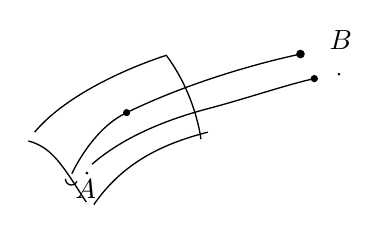
\begin{tikzpicture}[x=.80cm,y=.80cm,line width=.48pt]
\draw (0,.72) .. controls (.46,1.27) and (1.36,1.70) .. (2.09,1.94)
 .. controls (2.36,1.58) and (2.57,1.09) .. (2.64,.61);
\draw (2.75,.72) .. controls (2.05,.54) and (1.41,.25) .. (.94,-.43);
\draw (.82,-.39) .. controls (.46,.16) and (.29,.48) .. (-.10,.58);
\draw (.59,.06) .. controls (.74,.37) and (1.04,.83) .. (1.46,1.03)
 .. controls (2.18,1.38) and (3.16,1.73) .. (4.22,1.96);
\draw (.91,.21) .. controls (1.39,.63) and (2.06,.91) .. (2.74,1.09)
 .. controls (3.35,1.25) and (4.02,1.48) .. (4.44,1.57);
\draw (.49,-.02) arc[start angle=177,end angle=337,radius=.095];
\fill (.83,.07) circle[radius=.55pt];
\fill (1.46,1.03) circle[radius=1.30pt];
\draw[fill=black] (4.22,1.96) circle[radius=1.30pt];
\draw[fill=black] (4.44,1.57) circle[radius=1.05pt];
\fill (4.83,1.64) circle[radius=.52pt];
\node[below right,inner sep=.4pt] at (.62,-.01) {$A$};
\node[above right,inner sep=1pt] at (4.63,1.98) {$B$};
\end{tikzpicture}}\endgroup\par
The small strokes at $A$ leave the connection of the two curves unresolved.}
\end{GelfandAdjacentEvidence}
\begin{GelfandAdjacentEvidence}{GELFAND-P001017}{5}


$A$ --- a point on the surface.

$B$ --- an arbitrary point off the surface.

look for extremals (the geodesics break off)

A. \underline{The space of lines in $\mathbb{R}^3$ has a natural symplectic structure!}

B. \underline{Generalization}: \underline{the space of extremals of any variational problem has a symplectic structure}.

A. it is $T^*\mathbb{R}^2$ (Arnold’s explanation)

\underline{Example}:

\SourceFigure{GELFAND-P001017}{sphere-extremals}{%
\begingroup\color{black}\GelfandFitDiagram{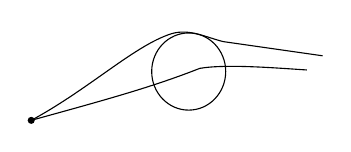
\begin{tikzpicture}[x=1cm,y=1cm]
\fill (0,0) circle (0.045);
\draw (2.0,.62) ellipse (.47 and .49);
\draw (0,0) .. controls (.74,.40) and (1.31,.95) .. (1.78,1.10)
 .. controls (2.01,1.17) and (2.23,1.05) .. (2.44,1.00) -- (3.70,.82);
\draw (0,0) .. controls (.94,.26) and (1.53,.42) .. (2.14,.66)
 .. controls (2.48,.72) and (3.17,.66) .. (3.50,.64);
\end{tikzpicture}}\endgroup}
\end{GelfandAdjacentEvidence}
\begin{GelfandAdjacentEvidence}{GELFAND-P001017}{6}


a point and a sphere: a two-dimensional manifold of extremals arises.

\begin{center}--- $\cdot$ ---\end{center}
Consider the space of binary forms $\bigl\{\sum_0^{2n-1}a_i x^i y^{2n-1-i}\bigr\}$
and on it the representation of the group $SL_2(\mathbb{R})$.
\Incomplete{GELFAND-P001017}{binary-cancelled-line}{The sentence is crossed out. It may begin “This space” or “On the space”. Its full reading remains unresolved.}
\end{GelfandAdjacentEvidence}
\begin{GelfandAdjacentEvidence}{GELFAND-P001017}{7}

At $y=1$ --- simply a polynomial of degree $2n-1$.

$w=\dfrac{x}{y}$ --- an inhomogeneous coordinate.
Write the polynomial in this variable using Darboux coordinates:
\[
\frac{q_1w^{2n-1}}{(2n-1)!}+\ldots+\frac{q_nw^n}{n!}
+\frac{p_nw^{n-1}}{(n-1)!}\mathrel{\boxed{?}}
\frac{p_{n-1}w^{n-2}}{(n-2)!}+\ldots+(-1)^{n-1}\frac{p_1w^0}{0!}
\]
\Unclear{GELFAND-P001017}{polynomial-overwritten-sign}{The sign before the term with $p_{n-1}$ is overwritten. Two horizontal strokes and a lower vertical stroke are visible. The final sign remains unresolved.}
\end{GelfandAdjacentEvidence}



\Needspace{7\baselineskip}
\SourcePage{GELFAND-P001018}{unlabelled}
\[
\omega=\sum_{i=1}^{n}dp_i\wedge dq_i
\]
The action of $SL_2(\mathbb{R})$ preserves the form.

$w\mapsto w+t$ \underline{is a Hamiltonian flow}; since it comes from
$\begin{pmatrix}1&t\\0&1\end{pmatrix}$

Hamiltonian:
\[
h=q_n^2/2-q_{n-1}p_n-\ldots-q_1p_2
\]
$q_1$ --- a first integral.

Consider the reduction $q_1=1$ and the space of characteristics on it.

(we also take $p_1=1$ --- this is a convention)

\underline{Question of I. Goldsheid.}

Consider a symplectic space with canonical basis $e_1,\ldots,e_n,f_1,\ldots,f_n$

Let $L$ be a Lagrangian plane in it.
Is there a (Lagrangian) plane $L_1$, spanned by vectors $\varphi_1,\ldots,\varphi_n$, where
$\varphi_j=\alpha_j e_j+\beta_j f_j$, such that
\[
\rho(L,L_1)\le 1/\sqrt{2}
\]
(it suffices to have $<1-\varepsilon$, where $\varepsilon>0$ is independent of the dimension)

Here $\rho(L,L_1)=\|P_L-P_{L_1}\|$, where the (operator) norm is taken in the standard Euclidean metric in the basis
$e_1,\ldots,e_n,f_1,\ldots,f_n$.

It is asserted that $\exists\varphi_j$ such that $\sin(\widehat{\varphi_j,L})\le 1/\sqrt{2}$.


\Needspace{7\baselineskip}
\begin{GelfandAdjacentEvidence}{GELFAND-P001019}{1}
\SourcePage{GELFAND-P001019}{unlabelled}
\underline{\underline{5/IV/82}}\qquad\underline{Gelfand seminar.}

\underline{\underline{Wodzicki}}

$M$ --- a manifold (possibly with boundary $\partial M$)

$D$ --- a system of differential equations on $M$:
\[
(1)\qquad D:C^\infty(M,E)\longrightarrow C^\infty(M,E)
\]
\underline{elliptically determined} ($\sigma_D$ is invertible).

\Unclear{GELFAND-P001019}{eq-two-cancel}{A mark before the equation number (2) is crossed out. Its reading remains unresolved.}
\end{GelfandAdjacentEvidence}

\[
(2)\qquad \operatorname{index}D=\dim\ker D-\dim\operatorname{Coker}D
=\int_M\alpha_0(x)\qquad\text{(Atiyah--Singer)}
\]
[Below $\alpha_0(x)$: \underline{density}.]

(2) --- an example of a local formula.

The coefficient $\alpha_0$ is expressed in terms of the symbol. Here there naturally appears a $\zeta$-function
\[
(3)\qquad \zeta_A(s)=\sum_{\lambda\in\operatorname{Spec}A}\lambda^{-s}
\]
\[
A=D^*D,\quad DD^*.
\]
\[
z_j=\frac{n-j}{m}\quad\text{--- poles},\qquad
n=\dim M,\quad m=\text{order of }A.
\]
\[
z_j=0,-1,-2,\ldots\quad\text{--- \underline{there are no poles}.}
\]
\[
\int_M\underbrace{\zeta_A(0;x)}_{\text{density}}=\zeta(0);
\qquad \zeta_A(0;x)\text{ can be computed explicitly}
\]
\[
(4)\qquad \operatorname{index}D=\zeta_{1+D^*D}(0)-\zeta_{1+DD^*}(0)
\]


\Needspace{7\baselineskip}
\begin{GelfandAdjacentEvidence}{GELFAND-P001020}{1}
\SourcePage{GELFAND-P001020}{unlabelled}
\[
(5)\qquad
\zeta_A(0;x)=-\frac1m\int_{|\xi|=1}d\xi'
  \int_0^\infty\operatorname{tr} b^0_{-m-n}(x,\xi,\lambda)\,d\lambda
\]
\Unclear{GELFAND-P001020}{eq-five-cancel}{A sign or factor is crossed out between the equals sign and $-1/m$.}
\end{GelfandAdjacentEvidence}
\begin{GelfandAdjacentEvidence}{GELFAND-P001020}{2}

\Unclear{GELFAND-P001020}{parametrix-superscript}{A small oval is written above $b$. It could be $0$, $o$ or $\circ$.}
\end{GelfandAdjacentEvidence}
\begin{GelfandAdjacentEvidence}{GELFAND-P001020}{3}


[A line from $b^0_{-m-n}$ to the explanation on the right:]
component of the symbol of the parametrix for $(A-\lambda)$ in some chart.

$\zeta_A(0;x)\,dx$ --- a density (!) --- this is not obvious.

Suppose $\partial M\ne\varnothing$.
\SourceFigure{GELFAND-P001020}{upper-boundary-condition}{The manuscript has $\partial M\ne\varnothing$.}
\end{GelfandAdjacentEvidence}
\begin{GelfandAdjacentEvidence}{GELFAND-P001020}{4}


$D$ --- the signature operator (Dirac)

For this operator:
\[
(6)\qquad \operatorname{index}D=\operatorname{sign}M
\]
\[
(7)\qquad \int_M L_k(p)=\operatorname{index}D=\int_M\alpha_0(x)
\]
\[
D:\Omega_+\longrightarrow\Omega_-
\]
$\Omega_\pm$ --- forms even (odd) under the involution
$\tau=i^{np+n+1}*$ (on $p$-forms).
\[
(8)\qquad d+d^*=D|_{\Omega_+}:\Omega_+\longrightarrow\Omega_-.
\]

\underline{Example} (I. M. G.)
\[
(9)\qquad
\begin{pmatrix}0&\operatorname{div}\\\operatorname{grad}&\operatorname{rot}\end{pmatrix}^{2}
=\Delta\underset{\text{identity matrix}}{I}\qquad\text{(in }R^4\text{)}
\]

\[
(10)\qquad \underline{\text{Theorem.}}\quad L_k(p)=\alpha_0(x)
\qquad\text{(Atiyah--Bott--Patodi)}
\]
\[
n=4\quad\Rightarrow\quad\alpha_0(x)=\frac13p_1
\]

\underline{The case}
\Unclear{GELFAND-P001020}{kahler-cancel}{Marks before $D$ are crossed out.}
\end{GelfandAdjacentEvidence}
\begin{GelfandAdjacentEvidence}{GELFAND-P001020}{5}

\underline{$D=\bar\partial$} and $\overset{\text{metric}}{M}$ is
Kähler
$\Rightarrow$ local agreement of $\alpha_0(\ldots)$ and the component
of the Todd genus $T(p)$ (in general this is \underline{false}).
\Unclear{GELFAND-P001020}{todd-abbreviation}{The abbreviation before “Todd genus” most likely reads «соств.».}
\end{GelfandAdjacentEvidence}
\begin{GelfandAdjacentEvidence}{GELFAND-P001020}{6}


That is, there are two local formulas that do not coincide.

$\partial M\ne\varnothing\Rightarrow$ there is also a \underline{signature}
(degenerate form on middle cohomology, with zeros disregarded)
\[
(11)\qquad
\underset{\substack{\text{topological}\\\text{invariant}}}{\operatorname{sign}M}
=\underbrace{\int_M L_k(p)}_{\text{local formula}}
-\underbrace{\eta(\partial M)}_{\substack{\text{depends}\\\text{on the metric}\\\text{at the boundary}}}
\]
(the metric near the boundary --- \underline{is a product}).

\underline{I. M. G. Problem}: is $\operatorname{sign}$ ---
\underline{the only additive} invariant for manifolds
\Unclear{GELFAND-P001020}{question-cancel}{A short word before “with” is crossed out.}
\end{GelfandAdjacentEvidence}
\begin{GelfandAdjacentEvidence}{GELFAND-P001020}{7}

with \underline{boundary}?

\begin{center}--- $\cdot$ ---\end{center}
Pass to the double:
\SourceFigure{GELFAND-P001020}{double-diagram}{%
\begingroup\color{black}\GelfandFitDiagram{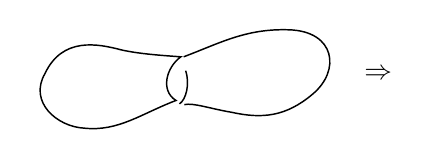
\begin{tikzpicture}[x=.88cm,y=.88cm,line width=.53pt]
\draw (0,.27) .. controls (.25,.80) and (.76,.70) .. (1.10,.61)
 .. controls (1.37,.55) and (1.69,.53) .. (1.96,.51)
 .. controls (1.75,.36) and (1.66,.02) .. (1.89,-.12)
 .. controls (1.39,-.31) and (1.06,-.57) .. (.57,-.52)
 .. controls (.17,-.50) and (-.24,-.14) .. (0,.27);
\draw (2.00,.51) .. controls (2.53,.71) and (2.90,.92) .. (3.52,.90)
 .. controls (4.19,.88) and (4.27,.31) .. (3.86,-.03)
 .. controls (3.48,-.35) and (3.14,-.39) .. (2.69,-.29)
 .. controls (2.39,-.24) and (2.14,-.15) .. (2.01,-.18);
\draw (2.03,.31) .. controls (2.09,.12) and (2.04,-.10) .. (1.94,-.17);
\node at (4.81,.25) {$\Rightarrow$};
\end{tikzpicture}}\endgroup\par
There is a gap at the top of the right-hand stroke of the seam.}
\end{GelfandAdjacentEvidence}

By Hirzebruch’s theorem (equation (7)), we see
that $\eta(\partial M)$ \underline{is independent of the filling}.

(12)\qquad $\eta(\partial M)$ --- a nonlocal invariant!!

Locality $\Rightarrow$ multiplicativity
(\underline{with respect to} [inserted above the line] passing to coverings)

There are examples (lens spaces) where this fails.


\Needspace{7\baselineskip}
\begin{GelfandAdjacentEvidence}{GELFAND-P001021}{1}
\SourcePage{GELFAND-P001021}{58}
(13) \underline{Theorem.} (Atiyah--Patodi--Singer)

$N=\partial M$, $D$ --- a first-order system
\begin{equation}
D=\frac{\partial}{\partial u}+A,\qquad A\text{ --- an operator on }\partial M
\tag{14}
\end{equation}
(near the boundary)

Let $A$ \underline{be normal} with spectrum disjoint from a conical neighbourhood of $i\mathbb R$.
\Unclear{GELFAND-P001021}{spectrum-cancel}{Between “not” and “intersecting” is a crossed-out abbreviation, possibly «сод.» or «соб.».}
\end{GelfandAdjacentEvidence}
\begin{GelfandAdjacentEvidence}{GELFAND-P001021}{2}


\SourceFigure{GELFAND-P001021}{margin-spectrum}{%
\begingroup\color{black}\GelfandFitDiagram{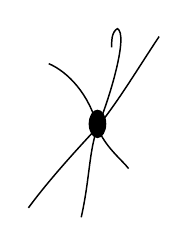
\begin{tikzpicture}[x=.86cm,y=.86cm,line width=.53pt]
\draw (-.24,-1.33) .. controls (-.11,-.74) and (-.13,-.38) .. (0,0)
 .. controls (.17,.40) and (.47,1.38) .. (.29,1.46);
\draw (.30,1.46) .. controls (.20,1.41) and (.21,1.25) .. (.21,1.18);
\draw (-1.02,-1.19) .. controls (-.69,-.74) and (-.23,-.25) .. (0,0)
 .. controls (.35,.45) and (.54,.78) .. (.91,1.34);
\draw (-.72,.94) .. controls (-.44,.82) and (-.12,.49) .. (0,0)
 .. controls (.11,-.29) and (.36,-.48) .. (.46,-.61);
\fill (0,.05) ellipse (.13 and .21);
\end{tikzpicture}}\endgroup}
\end{GelfandAdjacentEvidence}
\begin{GelfandAdjacentEvidence}{GELFAND-P001021}{3}


Then $\exists$ elliptic boundary conditions for $D$.

$P_A$ --- the projector onto the eigenvalues of $A$ with $\operatorname{Re}A\geq 0$.
\SourceFigure{GELFAND-P001021}{projection-real-part}{The condition reads $\operatorname{Re}A\geq 0$.}
\end{GelfandAdjacentEvidence}
\begin{GelfandAdjacentEvidence}{GELFAND-P001021}{4}


\begin{equation}
\left\{
\begin{aligned}
Df\\
P_A(f|_A)=0
\end{aligned}
\right\}
\quad\text{--- }\underline{\text{a nonlocal boundary-value problem}}
\tag{15}
\end{equation}
\SourceFigure{GELFAND-P001021}{boundary-restriction}{The restriction subscript in (15) is written $A$.}
\end{GelfandAdjacentEvidence}
\begin{GelfandAdjacentEvidence}{GELFAND-P001021}{5}


a local problem does not always exist.

But a nonlocal problem always exists!!
\Unclear{GELFAND-P001021}{nonlocal-cancel}{A mark after “nonlocal” is crossed out.}
\end{GelfandAdjacentEvidence}
\begin{GelfandAdjacentEvidence}{GELFAND-P001021}{6}


Then:
\begin{equation}
\operatorname{index}D=\int\alpha_0(x)-\frac{h_0+\eta(A)}{2},
\tag{16}
\end{equation}
where

$h_0=\dim$ (space of purely imaginary eigenvalues).
\Unclear{GELFAND-P001021}{kernel-cancel}{The entry after $\dim$ is crossed out. It may read $\operatorname{Ker}A$ or $\operatorname{Ker}A_0$.}
\end{GelfandAdjacentEvidence}
\begin{GelfandAdjacentEvidence}{GELFAND-P001021}{7}

\begin{equation}
\eta(A)\equiv\eta(0,A),\qquad
\eta(s,A)=\sum_{\lambda\in\operatorname{Spec}A}
\operatorname{sign}\operatorname{Re}\lambda\,
|\operatorname{Re}\lambda|^{-s}
\tag{17}
\end{equation}

\underline{Point}: generalization of the $L$-function.

In A.-P.-S. \underline{$A$ --- a self-adjoint operator}
\Unclear{GELFAND-P001021}{attribution-cancel}{The entry before A.-P.-S. is crossed out. It may read «Водз.» or «Водз».}
\end{GelfandAdjacentEvidence}
\begin{GelfandAdjacentEvidence}{GELFAND-P001021}{8}


\underline{Theorem.} $A$ --- an elliptic operator.
\[
\int_{N\times I}L_k(p)=\eta_{p_1}-\eta_{p_2}
\]
\Unclear{GELFAND-P001021}{cylinder-formula-symbol}{The handwritten letters in $L_k(p)$ and the subscripts of $\eta$ resemble $p$. The subscripts may be $\rho$.}
\end{GelfandAdjacentEvidence}
\begin{GelfandAdjacentEvidence}{GELFAND-P001021}{9}


\SourceFigure{GELFAND-P001021}{cylinder-diagram}{%
\begingroup\color{black}\GelfandFitDiagram{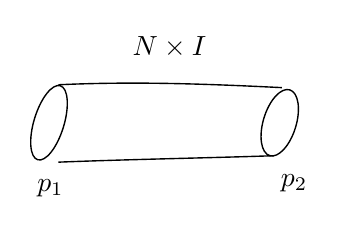
\begin{tikzpicture}[x=.91cm,y=.91cm,line width=.5pt]
\draw[rotate around={-17:(0,0)}] (0,0) ellipse (.21 and .54);
\draw[rotate around={-17:(3.22,0)}] (3.22,0) ellipse (.23 and .48);
\draw (.13,.53) .. controls (1.21,.58) and (2.24,.54) .. (3.25,.49);
\draw (.13,-.55) .. controls (1.15,-.51) and (2.28,-.49) .. (3.14,-.46);
\node at (1.68,1.05) {$N\times I$};
\node at (.02,-.91) {$p_1$};
\node at (3.42,-.84) {$p_2$};
\end{tikzpicture}}\endgroup\par
The end labels read $p_1,p_2$ or $\rho_1,\rho_2$.}
\end{GelfandAdjacentEvidence}



\Needspace{7\baselineskip}
\begin{GelfandAdjacentEvidence}{GELFAND-P001022}{1}
\SourcePage{GELFAND-P001022}{unlabelled}
\underline{12/IV/82}\qquad\underline{Gelfand seminar.}

\underline{Wodzicki.} (\underline{Mariusz})

$X$ --- a compact manifold with boundary.
\SourceFigure{GELFAND-P001022}{manifold-abbreviation}{The manuscript abbreviates “manifold” as «мн-зие».}
\end{GelfandAdjacentEvidence}
\begin{GelfandAdjacentEvidence}{GELFAND-P001022}{2}


(1) $D\colon C^\infty(X,E)\to C^\infty(X,F)$
is a first-order elliptic system which (differential)
near $\partial X$ takes the form
\[
(2)\qquad D=\frac{\partial}{\partial u}+A,\qquad
A\text{ --- an operator on the boundary}
\]
\[
(3)\qquad A\colon C^\infty(Y,E|_Y)\longrightarrow C^\infty(Y,F|_Y)
\]

\SourceFigure{GELFAND-P001022}{margin-spectrum}{%
\begingroup\color{black}\GelfandFitDiagram{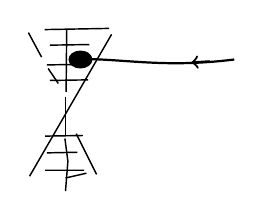
\begin{tikzpicture}[x=.76cm,y=.76cm,line width=.52pt]
\draw (-.08,-1.05) -- (-.04,-.55) -- (-.09,-.17);
\draw (-.08,-.11) -- (-.08,.53);
\draw (-.07,.61) -- (-.06,1.64);
\draw (-.68,-.80) -- (.69,1.57);
\draw (-.70,1.60) -- (-.48,1.19);
\draw (-.37,1.00) -- (-.20,.75);
\draw (.10,-.09) -- (.44,-.77);
\draw (-.43,1.65)--(.65,1.67)
      (-.34,1.39)--(.32,1.40)
      (-.39,1.06)--(.30,1.07)
      (-.34,.80)--(.30,.81)
      (-.42,-.13)--(.21,-.12)
      (-.39,-.41)--(.12,-.40)
      (-.42,-.70)--(.23,-.70)
      (-.08,-.83)--(.27,-.75);
\fill (.17,1.15) ellipse (.20 and .15);
\draw[<- ,thick] (.18,1.16) .. controls (.98,1.15) and (1.61,1.01) .. (2.74,1.15);
\draw[<- ,thick] (2.02,1.10)--(2.33,1.12);
\end{tikzpicture}}\endgroup\par
[Label with arrow:] only finitely many eigenvalues of the operator $A$.\par
Dense strokes at the tip obscure the exact joins.}
\end{GelfandAdjacentEvidence}
\begin{GelfandAdjacentEvidence}{GELFAND-P001022}{3}


Boundary conditions:
\[
(4)\qquad P_+f|_Y=0,
\]
$P_+$ --- the projector onto the positive eigenfunctions of the operator $A$.
\Unclear{GELFAND-P001022}{projection-cancellation}{A mark is crossed out between the words abbreviated as “eigenfunctions”.}
\end{GelfandAdjacentEvidence}
\begin{GelfandAdjacentEvidence}{GELFAND-P001022}{4}


(5) \underline{Theorem} (Atiyah--Patody--Singer)

1974 and followers
\Unclear{GELFAND-P001022}{theorem-year-connector}{The small word after “1974” most likely reads “and”.}
\end{GelfandAdjacentEvidence}
\begin{GelfandAdjacentEvidence}{GELFAND-P001022}{5}


suppose

1) $A$ \underline{is normal} with respect to the Riemannian metric \underline{on the boundary}
\qquad $(A^*A=AA^*)$
\[
(6)\qquad \operatorname{index}D=\int_X\alpha_0(x)\,dx
-\frac{h(A)+\eta(A)}2
\]
\[
(7)\qquad \eta(A,s)=\sum\operatorname{sign}\operatorname{Re}\lambda\cdot
|\operatorname{Re}\lambda|^{-s},\qquad \eta(A)=\eta(A,0)
\]
\Unclear{GELFAND-P001022}{eq-seven-number}{The number beside the formula for $\eta(A,s)$ is overwritten. The top stroke and the numbering sequence support (7).}
\end{GelfandAdjacentEvidence}

\[
(8)\qquad h(A)=\dim\left\{\begin{gathered}
\text{imaginary}\\\text{eigenvalues of }A
\end{gathered}\right\}
\]


\Needspace{7\baselineskip}
\begin{GelfandAdjacentEvidence}{GELFAND-P001023}{1}
\SourcePage{GELFAND-P001023}{64}
\underline{Proof.} Use the formula:
\[
(9)\qquad \operatorname{index}D=
\begin{array}[t]{c}
\operatorname{Tr}e^{-tD^*D}\\
\vert\vert\vert\\
\displaystyle\sum_{\lambda\in\operatorname{Spec}D^*D}e^{-t\lambda}
\end{array}
-
\begin{array}[t]{c}
\operatorname{Tr}e^{-tDD^*}\\
\Vert\\
\displaystyle\sum_{\mu\in\operatorname{Spec}DD^*}e^{-t\mu}
\end{array}
\]

\SourceFigure{GELFAND-P001023}{upper-left-figure}{%
\begingroup\color{black}\GelfandFitDiagram{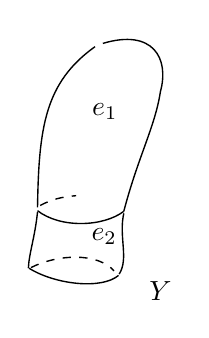
\begin{tikzpicture}[x=.83cm,y=.83cm,line width=.5pt]
\draw (0,.73) .. controls (.02,1.95) and (.11,2.64) .. (.88,3.19);
\draw (1.00,3.24) .. controls (1.77,3.47) and (2.02,3.01) .. (1.88,2.50)
 .. controls (1.80,1.97) and (1.54,1.51) .. (1.32,.67);
\draw (0,.68) .. controls (.35,.41) and (1.00,.43) .. (1.32,.67);
\draw (0,.66) .. controls (-.04,.27) and (-.13,.03) .. (-.14,-.20);
\draw (1.32,.64) .. controls (1.24,.28) and (1.40,-.05) .. (1.25,-.29);
\draw (-.13,-.20) .. controls (.27,-.45) and (.98,-.53) .. (1.24,-.31);
\draw[dashed] (-.10,-.19) .. controls (.32,.02) and (.92,.04) .. (1.17,-.24);
\draw[dashed] (.04,.76) .. controls (.23,.86) and (.37,.89) .. (.59,.91);
\node at (1.03,2.20) {$e_1$};
\node at (1.02,.29) {$e_2$};
\node at (1.88,-.55) {$Y$};
\end{tikzpicture}}\endgroup\par
The lower-right label reads $Y$. The rear arcs are broken.}
\end{GelfandAdjacentEvidence}
\begin{GelfandAdjacentEvidence}{GELFAND-P001023}{2}


\begin{center}--- $\cdot$ ---\end{center}

$A$ --- a self-adjoint elliptic operator.
\Unclear{GELFAND-P001023}{operator-cancellation}{A word is crossed out before “elliptic”.}
\end{GelfandAdjacentEvidence}
\begin{GelfandAdjacentEvidence}{GELFAND-P001023}{3}


\[
(10)\qquad \sum_{\lambda>0}\lambda^{-s}=\zeta_+(s),\qquad
\zeta_+(A)\text{ --- the value at }s=0.
\]

(11) $\zeta_+(A)<\infty$, but locally there is a \underline{residue}!!
(nonlocal functional)

\[
(12)\qquad \zeta_+(s)=\operatorname{Tr}(P_+A^{-s})
=\int_X\operatorname{Tr}(P_+A^{-s})(x,x)
\]
[At right: (there were singularities before taking the trace at $s=i$).]
\Unclear{GELFAND-P001023}{equation-12-margin}{The sign after $s=$ resembles $i$, with a faint separate stroke above it. The reading remains uncertain.}
\end{GelfandAdjacentEvidence}
\begin{GelfandAdjacentEvidence}{GELFAND-P001023}{4}


The local term has a residue, and $\displaystyle\int_X$ of this residue $=0$.
\Unclear{GELFAND-P001023}{local-abbreviation}{The abbreviation after “local” most likely means “term”. The last strokes are faint.}
\end{GelfandAdjacentEvidence}
\begin{GelfandAdjacentEvidence}{GELFAND-P001023}{5}


\[
(13)\qquad
\left\{
\begin{aligned}
\zeta(A)&=\zeta_+(A)+\zeta_-(A)\\
\eta(A)&=\zeta_+(A)-\zeta_-(A)
\end{aligned}
\right.
\]

\underline{I. M. G.}: in the work of Gabrielov, Gelfand and Fuks there are algebraic reasons for nonlocality.

\underline{The most remarkable problem is unsolved}: this is done to compute the values at the boundary of the forms of
\underline{Pontryagin}, but \underline{for general} classes there is nothing.
\SourceFigure{GELFAND-P001023}{pontryagin-abbreviation}{The manuscript abbreviates “values” as «знач.» before “at the boundary”.}
\end{GelfandAdjacentEvidence}
\begin{GelfandAdjacentEvidence}{GELFAND-P001023}{6}


\[
\begin{array}{l|l|l}
\underline{\text{Stredder}}&\text{J. Diff. Geometry}&\text{on natural differential operators.}\\
\underline{\text{Epstein}}&\underline{10}\ (1975),\ 645&\\
\text{(2 papers)}&&
\end{array}
\]

\begin{center}--- $\cdot$ ---\end{center}

\underline{Question of I. M. G.}: why require self-adjointness of $A$?

Let a domain and an operator on it be given, the operator $A$.

\SourceFigure{GELFAND-P001023}{boundary-region}{%
\begingroup\color{black}\GelfandFitDiagram{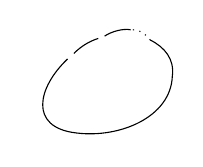
\begin{tikzpicture}[x=1cm,y=1cm]
\draw (1.42,1.25) .. controls (1.60,1.16) and (1.73,1.01) .. (1.70,.79)
 .. controls (1.68,.27) and (1.03,0) .. (.48,.07)
 .. controls (-.13,.14) and (-.01,.65) .. (.37,1.01);
\draw (.45,1.08) .. controls (.55,1.18) and (.66,1.24) .. (.76,1.27);
\draw (.84,1.30) .. controls (.93,1.36) and (1.08,1.40) .. (1.17,1.38);
\draw[dotted] (1.20,1.38) .. controls (1.31,1.38) and (1.37,1.31) .. (1.42,1.25);
\end{tikzpicture}}\endgroup}
\end{GelfandAdjacentEvidence}
\begin{GelfandAdjacentEvidence}{GELFAND-P001023}{7}


One constructs a theory of \underline{cobordisms}.

\underline{The invariant} [below it: $\eta(A)$] $A$ is constructed with a membrane stretched over the manifold.
\SourceFigure{GELFAND-P001023}{manifold-abbreviation}{The manuscript abbreviates “manifold” as «мн-зие».}
\end{GelfandAdjacentEvidence}


\begin{center}--- $\cdot$ ---\end{center}

But in the absence of a filling this has yet to be proved!!

\begin{center}--- $\cdot$ ---\end{center}

\[
(14)\qquad \alpha_0(x)=\zeta(D^*D+\varepsilon,x)-\zeta(DD^*+\varepsilon,x)
\]


\Needspace{7\baselineskip}
\begin{GelfandAdjacentEvidence}{GELFAND-P001024}{1}
\SourcePage{GELFAND-P001024}{unlabelled}
Formula for $\zeta(A,x)$
\begin{equation*}
\frac{1}{m}\int_{|\xi|=1}d\xi'\int_0^\infty
b^\circ_{-m-n}(x,\xi,\lambda)\,d\lambda
\tag{15}
\end{equation*}
\Unclear{GELFAND-P001024}{formula15-superscript}{In (15), a small broken oval above $b$ is rendered as a circle.}
\end{GelfandAdjacentEvidence}
\begin{GelfandAdjacentEvidence}{GELFAND-P001024}{2}


\SourceFigure{GELFAND-P001024}{seeley-sign-annotation}{%
\begin{tabular}{@{}l@{}c@{}}
\multicolumn{2}{@{}l@{}}{\(\uparrow\)}\\
Seeley has the wrong sign & \(\Vert\)
\end{tabular}}
\end{GelfandAdjacentEvidence}
\begin{GelfandAdjacentEvidence}{GELFAND-P001024}{3}


\SourceFigure{GELFAND-P001024}{angle-ray}{%
\begingroup\color{black}\GelfandFitDiagram{\begin{tikzpicture}[x=.86cm,y=.86cm]
\draw[->] (0,-.65)--(0,2.15);
\draw[->] (0,0)--(4.25,0);
\draw (0,0)--(2.05,2.15);
\draw (.65,0) arc (0:46:.65);
\node at (.88,.34) {$\theta$};
\end{tikzpicture}}\endgroup}
\end{GelfandAdjacentEvidence}
\begin{GelfandAdjacentEvidence}{GELFAND-P001024}{4}

\[
\zeta_\theta(s)=\sum\lambda^{-s}
\]
(with a cut along the ray at angle $\theta$)

\Unclear{GELFAND-P001024}{formula16-cancellation}{The crossed-out entry before (16) appears to read $\zeta_\theta(s)=$.}
\end{GelfandAdjacentEvidence}
\begin{GelfandAdjacentEvidence}{GELFAND-P001024}{5}

\begin{equation*}
\zeta_\theta^A(0,x)=-\frac{e^{i\theta}}{m}\int_{|\xi|=1}d\xi'
\int_0^\infty b^\circ_{-m-n}(x,\xi,e^{i\theta}\lambda)\,d\lambda
\tag{16}
\end{equation*}
(this is the correct formula)
\Unclear{GELFAND-P001024}{formula16-first-argument}{The first argument in (16) is overwritten. Both $0$ and $\theta$ are possible.}
\end{GelfandAdjacentEvidence}
\begin{GelfandAdjacentEvidence}{GELFAND-P001024}{6}

\Unclear{GELFAND-P001024}{formula16-superscript}{In (16), the superscript oval on $b$ is rendered as a circle.}
\end{GelfandAdjacentEvidence}
\begin{GelfandAdjacentEvidence}{GELFAND-P001024}{7}


\underline{I. M. G.} \underline{A remarkable operator in $\mathbb R^3$} (elliptic):
\begin{equation*}
\mathcal A\varphi=
\begin{pmatrix}0&\operatorname{div}\\\operatorname{grad}&\operatorname{rot}\end{pmatrix}
\begin{pmatrix}\varphi_0\\\vec\varphi\end{pmatrix}
=(\operatorname{div}\vec\varphi,\operatorname{grad}\varphi_0+\operatorname{rot}\vec\varphi)
\tag{17}
\end{equation*}
\[
\mathcal A^2=\begin{pmatrix}\Delta&0\\0&\Delta\end{pmatrix}.
\]
\SourceFigure{GELFAND-P001024}{operator17-square}{Both diagonal entries read $\Delta$.}
\end{GelfandAdjacentEvidence}
\begin{GelfandAdjacentEvidence}{GELFAND-P001024}{8}


\begin{center}--- $\cdot$ ---\end{center}

$A$ --- an elliptic operator on a closed manifold, the spectrum of $A$ does not fill a sector around the ray (ray of $\min$ growth)
\Unclear{GELFAND-P001024}{spectrum-word}{The word most likely means “fill”. “Meet” is also possible.}
\end{GelfandAdjacentEvidence}
\begin{GelfandAdjacentEvidence}{GELFAND-P001024}{9}


\[
\underbrace{\zeta_{\theta,A}(s)=\sum\lambda_\theta^{-s}}_{\vphantom{\lambda}}
\qquad \text{\underline{define using the ray}.}
\]
\SourceFigure{GELFAND-P001024}{comparison-rays}{%
\begingroup\color{black}\GelfandFitDiagram{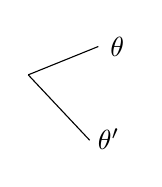
\begin{tikzpicture}[x=1cm,y=1cm]
\draw (0,.45)--(.89,.81);
\draw (0,.45)--(.78,-.38);
\node[right] at (.92,.81) {$\theta$};
\node[right] at (.76,-.37) {$\theta'$};
\end{tikzpicture}}\endgroup}
\end{GelfandAdjacentEvidence}
\begin{GelfandAdjacentEvidence}{GELFAND-P001024}{10}


Let $\theta'$ --- be another ray of $\min$ growth.
\[
\zeta_{\theta',A}(s)=\sum\lambda_{\theta'}^{-s}
\]
$\Rightarrow$ the spectrum lies in two sectors

\SourceFigure{GELFAND-P001024}{spectral-sectors-diagram}{%
\begingroup\color{black}\GelfandFitDiagram{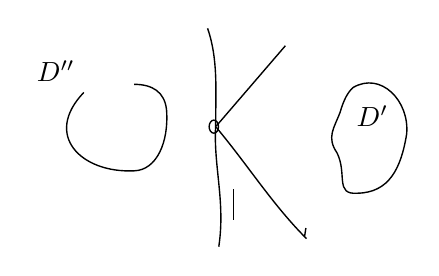
\begin{tikzpicture}[x=.79cm,y=.79cm,line width=.5pt]
\draw (-.02,1.66)..controls (.15,1.17) and (.11,.66)..(.11,.11)
..controls (.07,-.55) and (.27,-1.12)..(.16,-1.85);
\draw (.12,.09)--(1.23,1.38);
\draw (.11,.08)..controls (.63,-.54) and (1.02,-1.17)..(1.57,-1.72);
\draw (1.54,-1.68)--(1.56,-1.55);
\draw (.40,-.93)--(.40,-1.42);
\draw (.08,.08) ellipse (.075 and .105);
\draw (-2.01,.63)..controls (-2.67,-.06) and (-2.05,-.67)..(-1.20,-.63)
..controls (-.84,-.62) and (-.64,-.17)..(-.68,.35)
..controls (-.71,.64) and (-.91,.76)..(-1.20,.76);
\draw (2.32,.71)..controls (2.77,.97) and (3.23,.49)..(3.18,-.04)
..controls (3.09,-.59) and (2.90,-.98)..(2.39,-.99)
..controls (2.02,-1.02) and (2.23,-.68)..(2.06,-.34)
..controls (1.89,-.09) and (2.01,.05)..(2.11,.31)
..controls (2.17,.52) and (2.24,.64)..(2.32,.71);
\node at (-2.46,.98) {$D''$};
\node at (2.63,.25) {$D'$};
\end{tikzpicture}}\endgroup\par
The left contour has a gap. The tick at the bottom of the slanted stroke may be part of an arrow.}
\end{GelfandAdjacentEvidence}


(18) \underline{Theorem}.
\[
\rho(s)\overset{\mathrm{def}}{=}\zeta_\theta(A,s)-\zeta_{\theta'}(A,s)
\]
Then

a) $\rho(s)$ is meromorphic with residues at $z_j=\dfrac{-j+n}{m}$, $j=0,1,2,\ldots$

b) $z_j\in\mathbb Z\Rightarrow$ the residue vanishes microlocally!!

(elementary!)


\Needspace{7\baselineskip}
\begin{GelfandAdjacentEvidence}{GELFAND-P001025}{1}
\SourcePage{GELFAND-P001025}{65}
c)
\[
\begin{array}[t]{c}z_j\\\Vert\\\ell\end{array}
\in\mathbb Z\Rightarrow
\begin{array}[t]{c}\rho(z_j)\\\Vert\\\rho(\ell)\end{array}
\text{ is given by }\underline{\text{local formulas}}
\]
(a substantive assertion, --- also valid for pseudodifferential operators!)

\[
\begin{aligned}
(19)\qquad
\rho(i)&\overset{\mathrm{def}}{=}\int_X\rho_\ell(x)\,dx\\
&=-\frac{2\pi i}{m}\int_X dx\int_{|\xi|=1}d\xi'
\sum_{\lambda_\nu\in D'}\operatorname{Res}
\frac{\operatorname{tr}b^\circ_{m(i-1)-n}(x,\xi,\lambda)}{\lambda^\ell}
\end{aligned}
\]
\Unclear{GELFAND-P001025}{formula19-integer-symbol}{The argument of $\rho(i)$ resembles $i$, and the subscript of $\rho_\ell(x)$ resembles $\ell$. Part (c) uses $\ell$.}
\end{GelfandAdjacentEvidence}
\begin{GelfandAdjacentEvidence}{GELFAND-P001025}{2}

\Unclear{GELFAND-P001025}{formula19-b-superscript}{A broken oval above $b$ is rendered as a circle.}
\end{GelfandAdjacentEvidence}
\begin{GelfandAdjacentEvidence}{GELFAND-P001025}{3}

\Unclear{GELFAND-P001025}{formula19-power-symbol}{The index of $b$ appears to contain $i$, and the exponent of $\lambda$ appears to be $\ell$.}
\end{GelfandAdjacentEvidence}
\begin{GelfandAdjacentEvidence}{GELFAND-P001025}{4}


d) $\ell\in\mathbb Z_-=\{0,-1,-2,-3,-4,\ldots\}\Rightarrow\rho(\ell)=0$

(a stronger version of A.-P.-S.).

\underline{Hints} (for (d)):

The proof should cover more than just the residues at $0$, and should cover all integer points $>0$
\Unclear{GELFAND-P001025}{hint-word}{The word after “about” most likely reads “residues”.}
\end{GelfandAdjacentEvidence}
\begin{GelfandAdjacentEvidence}{GELFAND-P001025}{5}

\SourceFigure{GELFAND-P001025}{hint-integer-range}{The inequality in the hint reads \(>0\).}
\end{GelfandAdjacentEvidence}
\begin{GelfandAdjacentEvidence}{GELFAND-P001025}{6}


At the point $0$ it works out: use the Mahler transform (from the $p$-adic numbers):

\[
(20)\qquad
\zeta_\theta(-k,A+t)
=\underbrace{\sum_{\nu=0}^{k}\binom{k}{\nu}\zeta(\nu-k,A)t^\nu}
_{\text{\underline{\underline{polynomial}}:}}
+t^k\sum_{\mu=1}^{n}
\frac{(-1)^\mu\delta_\mu}{\binom{\mu+k}{k}\mu}
\]
\Unclear{GELFAND-P001025}{formula20-second-sum}{The second sum is preceded by $t^k$. No further power of $t$ is visible in the summand.}
\end{GelfandAdjacentEvidence}
\begin{GelfandAdjacentEvidence}{GELFAND-P001025}{7}


$\delta_\mu$ --- the residue at the point $\mu$ for the $\zeta$-function of the operator $A$

This is for first-order operators.

\[
\operatorname{Ker}A\ne\{0\}\Rightarrow
\text{instead of }\zeta(0)\text{ write }\zeta(0)+h_0(A)
\]
\SourceFigure{GELFAND-P001025}{kernel-bracket}{%
\begingroup\color{black}\GelfandFitDiagram{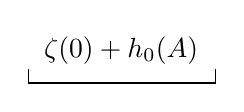
\begin{tikzpicture}[x=1cm,y=1cm]
\node at (1.18,.41) {$\zeta(0)+h_0(A)$};
\draw (0,.18)--(0,0)--(2.38,0)--(2.38,.18);
\end{tikzpicture}}\endgroup}
\end{GelfandAdjacentEvidence}
\begin{GelfandAdjacentEvidence}{GELFAND-P001025}{8}

($h_0(A)=\dim\operatorname{Ker}A$).

\Unclear{GELFAND-P001025}{mahler-cancellation}{The entry before “first sum” is crossed out and may read “Thm.”}
\end{GelfandAdjacentEvidence}

The first sum in (20) --- \underline{the Mahler transform.}

An automorphic function with respect to the Mahler transform extends to the $p$-adic domain.


\clearpage
\pdfbookmark[0]{Chapter 22}{gelfand-archive-chapter-22}
\section*{Chapter 22}
\Needspace{7\baselineskip}
